\documentclass[12pt, a4paper]{report}
\usepackage{dirtree}
\usepackage{microtype}
\usepackage{multirow}
\usepackage{makecell}
\usepackage{url}
\usepackage{graphicx}
\usepackage{float}
\usepackage[left=3cm,right=3cm,top=3cm,bottom=2.25cm]{geometry}
\usepackage{comment}
\usepackage{listings}
\usepackage{xcolor}
\usepackage{tabularx}
\usepackage{pdflscape}
\usepackage{subfig}
\usepackage{eso-pic}
\usepackage{color}
\usepackage{hyperref}
\hypersetup{
    colorlinks,
    citecolor=black,
    filecolor=black,
    linkcolor=black,
    urlcolor=black
}

\newcommand\BackgroundPic{%
\put(0,0){%
\parbox[b][\paperheight]{\paperwidth}{%
\vfill
\centering
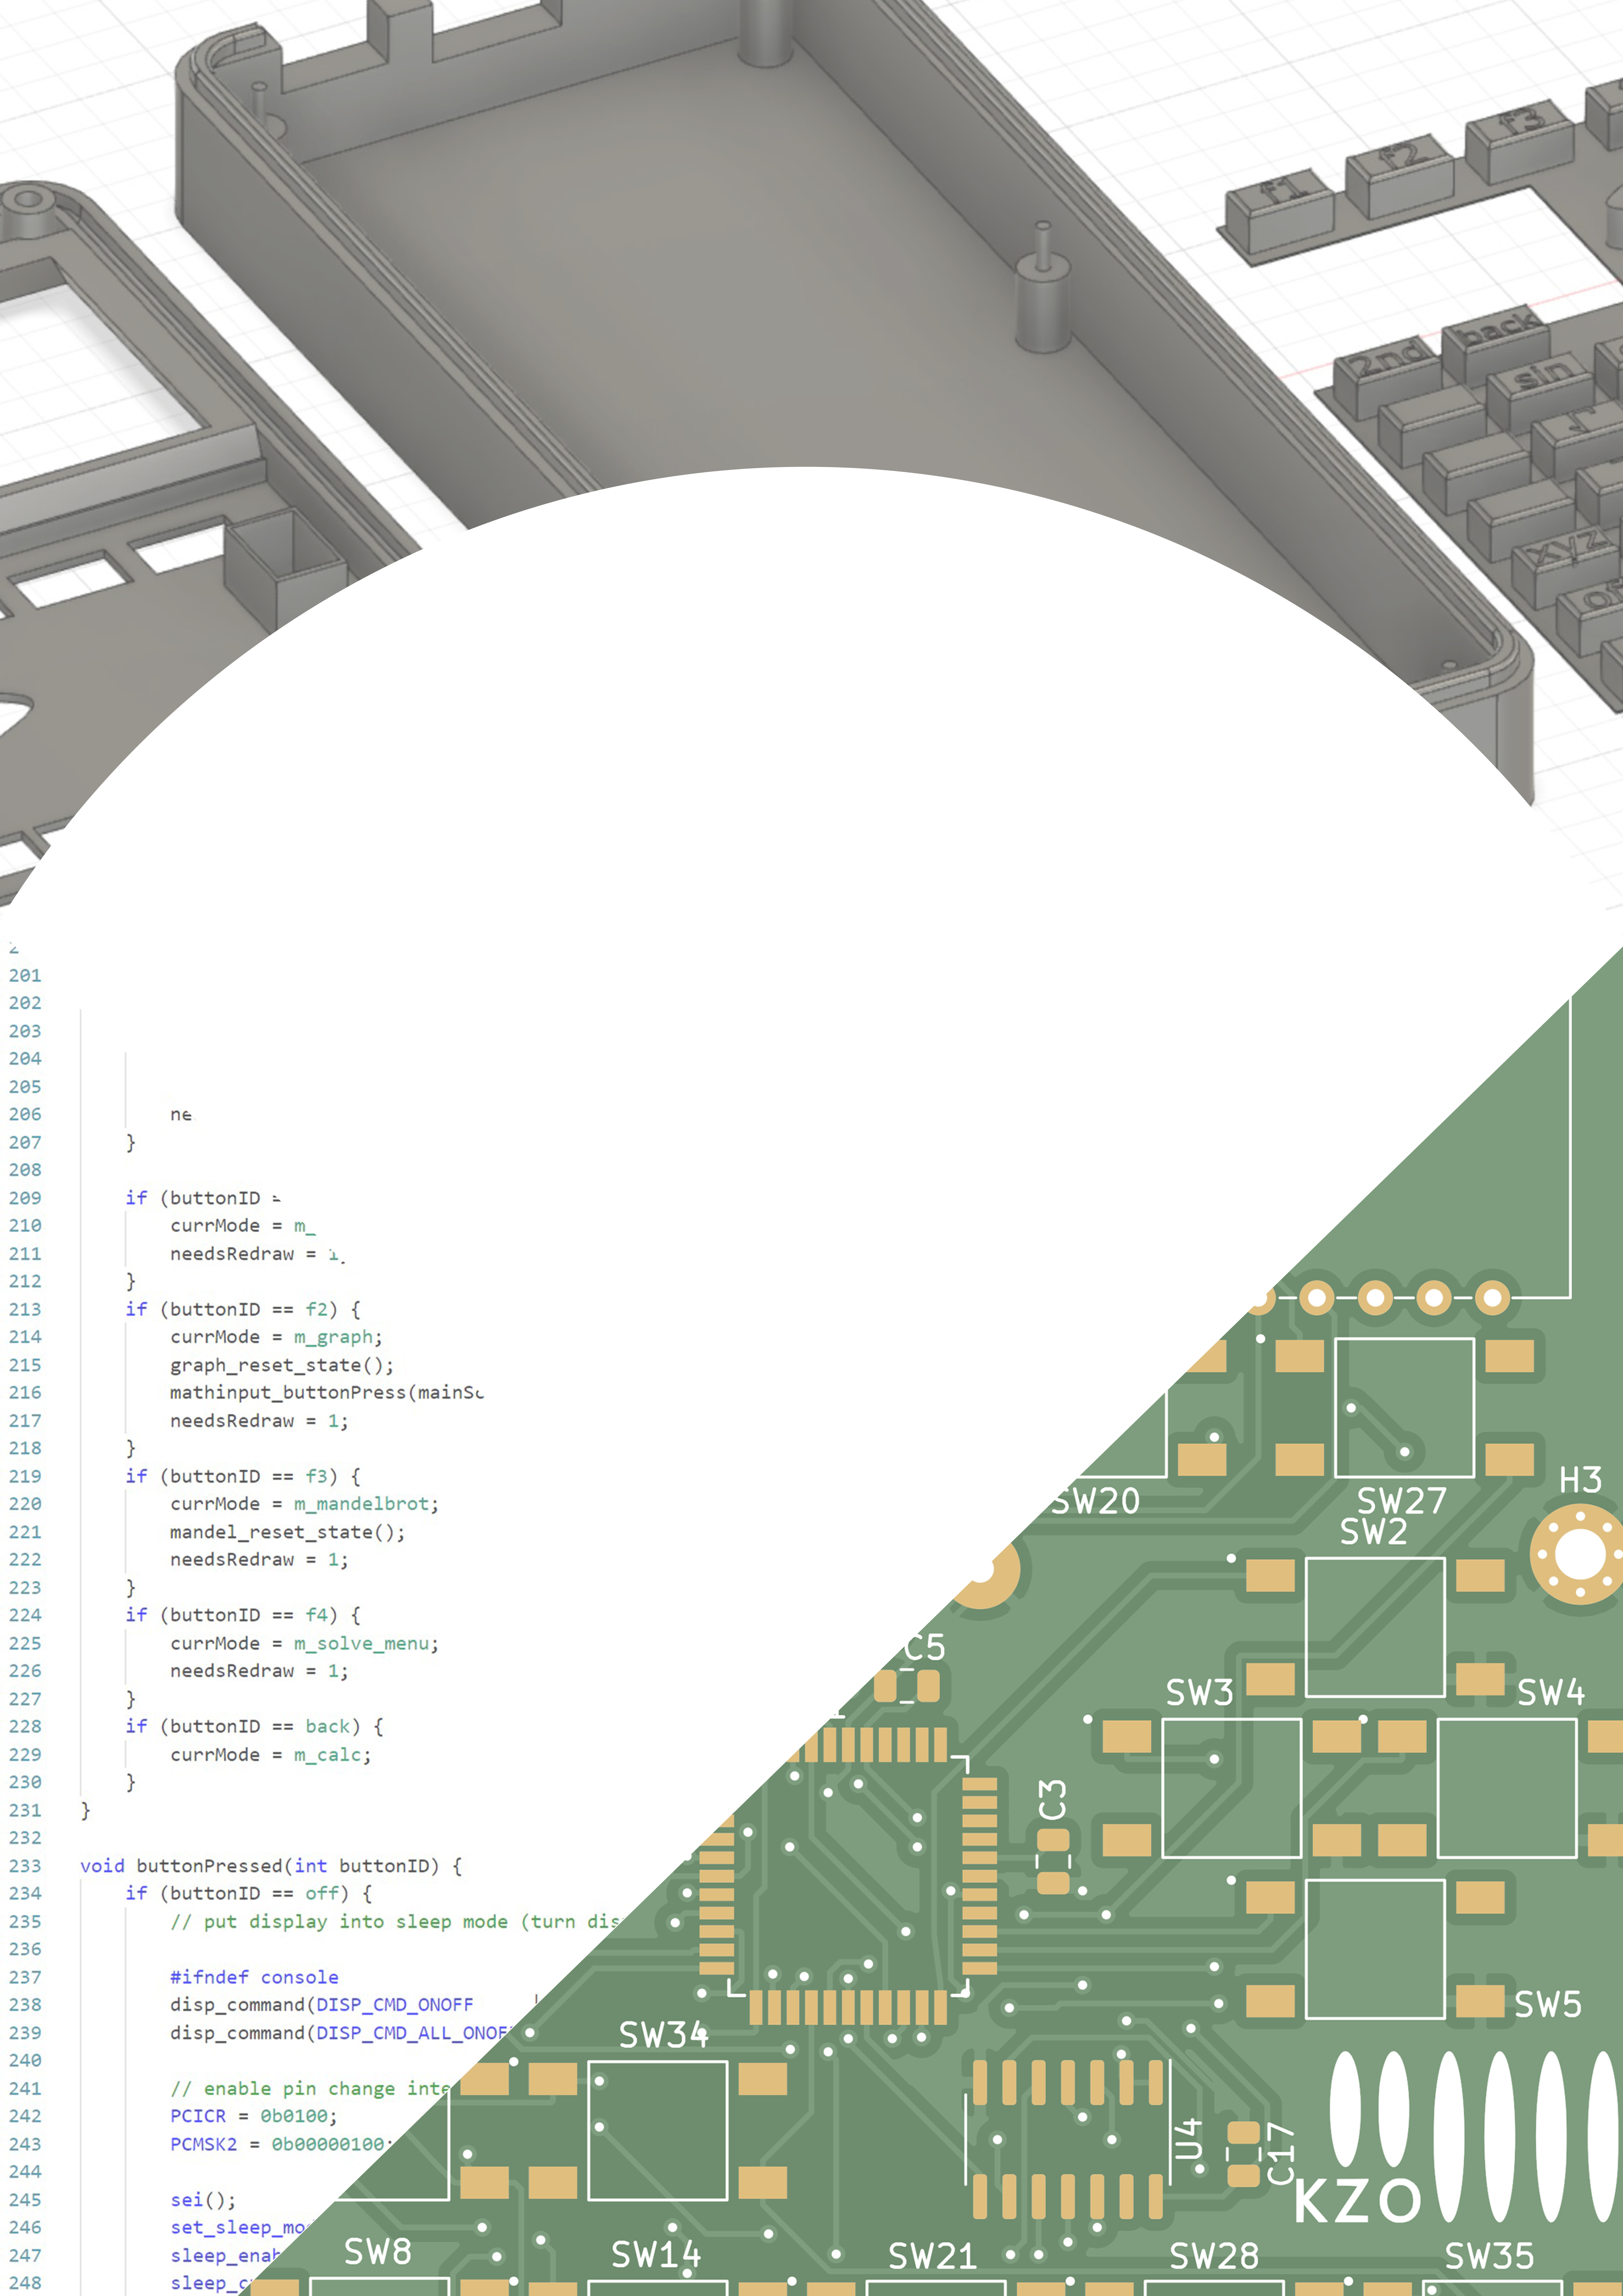
\includegraphics[width=0.98\paperwidth,height=0.98\paperheight,%
keepaspectratio]{assets/background.jpg}%
\vfill
}}}

\usepackage[ruled, vlined, longend]{algorithm2e}

\definecolor{codegreen}{rgb}{0,0.6,0}
\definecolor{codegray}{rgb}{0.5,0.5,0.5}
\definecolor{codepurple}{rgb}{0.58,0,0.82}
\definecolor{backcolour}{rgb}{0.95,0.95,0.92}

\lstdefinestyle{mystyle}{
    backgroundcolor=\color{backcolour},   
    commentstyle=\color{codegreen},
    keywordstyle=\color{magenta},
    numberstyle=\tiny\color{codegray},
    stringstyle=\color{codepurple},
    basicstyle=\ttfamily\footnotesize,
    breakatwhitespace=false,         
    breaklines=true,                 
    captionpos=b,                    
    keepspaces=true,                 
    numbers=left,                    
    numbersep=5pt,                  
    showspaces=false,                
    showstringspaces=false,
    showtabs=false,                  
    tabsize=1
}

\lstset{style=mystyle}

\addtolength{\skip\footins}{0.3cm}

\usepackage{german}
\selectlanguage{german}

\title{\ CALCKS\\ \Large Die Entwicklung eines Taschenrechners}
\author{Liam Braun, Klasse C6c\\
	Unter der Betreuung von Claudio Müller\\
	Kantonsschule Zürcher Oberland Wetzikon\\
	Maturitätsarbeit 2021}

\date{{18. Oktober 2020}}

\begin{document}

\AddToShipoutPicture*{\BackgroundPic}
\maketitle

\ClearShipoutPicture

\shipout\null

\selectlanguage{english}
\begin{abstract}
\selectlanguage{german}
Diese Arbeit beschreibt den Weg vom Entwurf bis zur Programmierung eines selbstentworfenen Taschenrechners. Thematisiert werden sowohl Fragestellungen bei der Entwicklung als auch technische Details bei der Umsetzung.
\end{abstract}

\selectlanguage{german}

\pagenumbering{arabic}

\tableofcontents

\newpage
\shipout\null

\chapter{Einleitung}
\section{Persönliches}
Schon sehr früh in meinem Leben war ich fasziniert von Technologie. Eine meiner Lieblingsbeschäftigungen war damals, mit dem wissenschaftlichen Taschenrechner, den mein Vater zu seiner Schulzeit an der KZO besass, zu spielen. Meine erste Programmiererfahrung fand auch auf diesem Gerät, dem SHARP EL-9300 statt. 
\begin{figure}[h]
	\centering
	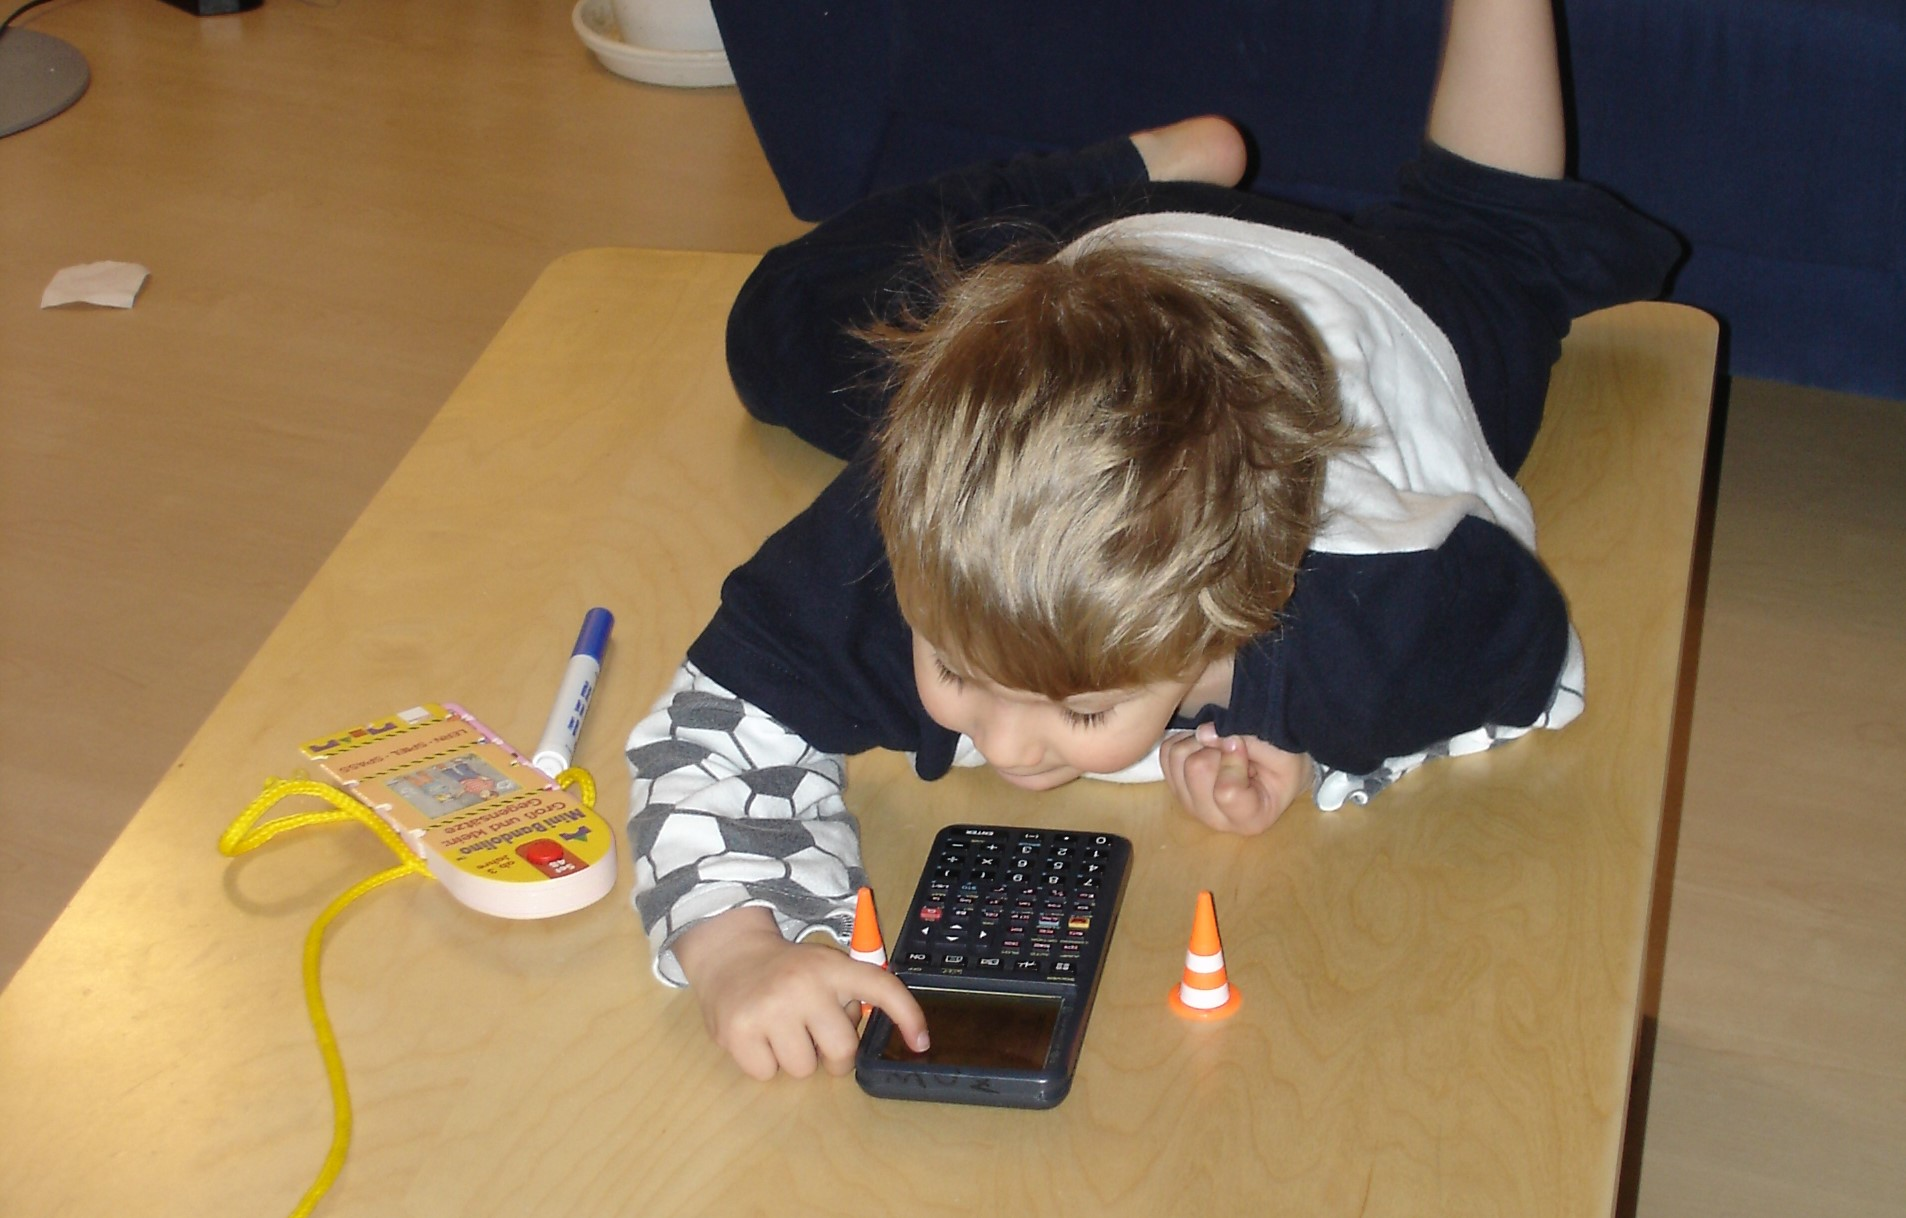
\includegraphics[width=\linewidth]{assets/me_with_calculator.jpg}
	\caption{Ich mit 3 Jahren, am Spielen mit dem Taschenrechner meines Vaters.}
	\label{fig:mewithcalc}
\end{figure}
\newpage
\section{Wahl des Projekts}
Bei der Wahl des Themas kamen verschiedene Bereiche auf, die ich in die Arbeit einbeziehen wollte. Zum einen war das Programmieren, egal ob als Teil eines Spiels, einer Website oder der Software eines Geräts, von Anfang der Fixpunkt, von dem aus ich das genauere Thema bestimmte. Ich war mir sicher, dass dies ein Bereich sei, auf den ich mich ohne Probleme über die acht Monate der Maturarbeit konzentrieren könnte, weil ich mich in meiner Freizeit seit etwa zehn Jahren mit dem Programmieren beschäftige. Ich wollte aber gleichzeitig meinen Horizont in der Informatikwelt erweitern und entschied mich deshalb, das Programmieren mit einem Hardwareprojekt zu kombinieren. Als ich mich an meine Taschenrechnerfaszination zurückerinnerte, war mir klar, was mein Maturprojekt sein soll.
\section{Ziele der Arbeit}
Zu Beginn der Arbeit hatte ich mir einige Erwartungen an das Endprodukt gesetzt:
\begin{itemize}
\item Der Taschenrecher sollte ein Matrix-LCD besitzen, damit er Funktionen plotten kann.
\item Der Taschenrecher sollte mindestens die Operationen Plus, Minus, Mal, Durch, Klammern, Wurzeln und Potenzen beherrschen, damit rechnen und Graphen zeichnen können.
\item Die Stromquelle des Taschenrechners sollte im Gerät integriert sein, entweder in Form einer gewöhnlichen Knopfzelle oder der eines Akkus.
\end{itemize}
Mir war am Endprodukt vor allem auch wichtig, dass ich einen Nutzen vom Taschenrechner hatte, also, dass der Taschenrechner Funktionen hat, die ein gewöhnlicher Taschenrechner nicht hat.
\section{Gliederung des schriftlichen Teils}
Der schriftliche Teil fokussiert sich mehrheitlich auf die Hardware. Grund dafür ist, dass auch wenn ein Grossteil der Arbeit am Taschenrecher Programmieren war, sind viele Teile des Programms nicht gross kommentierbar. Das Durchlesen des Quellcodes, der aus etwa 3'000 Zeilen Code besteht, ist dem Leser als freiwillige Aufgabe überlassen.
\\[\medskipamount]
Zuerst werden im Kapitel \textbf{Grundlagen} Begriffe erklärt, die vermehrt in der Arbeit vorkommen. In \textbf{Material und Methodik} wird der Arbeitsprozess aus meiner Sicht beschrieben. Das Kapitel \textbf{Technische Umsetzung} schaut das Endprodukt an und beschreibt, wie einzelne Teile davon funktionieren. Screenshots und Fotos vom Taschenrechner sind im Kapitel \textbf{Resultate} zu finden.
\chapter{Grundlagen}
\section{Komponenten in elektronischen Geräten}
\subsection{PCB}
Ein Printed Circuit Board, kurz PCB, ist eine meist grüne Platte, die sich in praktisch jedem elektronischen Gerät befindet. Auf sie werden die elektronischen Komponenten wie Prozessor, Knöpfe, Batterien usw. gelötet. Das Selbstherstellen einer solchen Leiterplatte ist bei simplen Schaltkreisen zwar möglich, aber ziemlich aufwendig. Wenn man auf dem Computer ein PCB designt, erstellt man als Erstes ein Schema, wo die elektronischen Komponenten möglichst klar und verständlich ausgelegt werden. Beim PCB-Layout hingegen ist der Fokus weniger bei der Verständlichkeit gegenüber dem Entwickler, sondern darauf, dass die Verbindungen zwischen Komponenten die richtige Breite haben und dass sie möglichst kurz und ohne viele Umwege sind.
\\[\medskipamount]
Das Schema ist für Menschen gedacht und soll die Idee des Zusammenspiels der Komponenten übersichtlich machen. Das PCB-Layout ordnet die Komponenten so an, dass sie optimal und zweckorientiert platziert sind. Ein USB-Port zum Beispiel könnte auf dem Schema beliebig platziert sein, aber auf dem PCB müsste er am Rand liegen, sodass er für den Nutzer gut erreichbar ist.
\subsection{Steckplatine}
Eine Steckplatine, auch Breadboard genannt, wird für den Prototypenbau verwendet und ist eine Plastikform, die in Reihen aufgeteilt ist. In jeder dieser Reihen hat ein Breadboard Klemmen, die sich über mehrere Löcher spannen und somit ein elektrisches Signal an andere Komponenten in derselben Reihe übertragen können.
Ganz links und rechts verlaufen meist je zwei Spalten, die dazu gedacht sind, an eine positive und negative Spannung anzuschliessen, aber grundsätzlich kann man beliebige Signale auf diese Reihen leiten.
\subsection{IC}
Ein IC, kurz für Integrated Circuit (Deutsch: Integrierter Schaltkreis), ist ein Schaltkreis, der Funktionen wie Timer, Speicher, Rechnen usw. aufweist und auf einem PCB verlötet wird oder auf ein Breadboard gesteckt wird. ICs kommen in vielen verschieden Formen und Grössen vor. Spricht man von den Namen dieser Formen, nennt man dies den Packaging-Typ des ICs.
\\[\medskipamount]
Die meisten ICs lassen sich in zwei Hauptgruppen unterteilen: SMT- und THM-ICs. SMT steht für ``Surface Mount Technology'' und bedeutet, dass eine SMT-Komponente auf Pads, die sich auf einem PCB befinden, platziert und angelötet werden. Pads sind kleine rechteckige Flächen auf einem PCB, worauf die Pins einer Komponente gelegt werden. THM steht für ``Through-Hole mounting'', was bedeutet, dass Komponenten dieser Art in durch das PCB durchgehende Löcher platziert und angelötet werden. Alternativ können diese Komponenten in die Löcher von Steckplatinen gesteckt werden, weshalb man für den Prototypbau auf Steckplatinen ausschliesslich THM-Komponenten verwendet.
\subsection{Speicher}
Es gibt verschiedene Arten, wie Daten in einem IC gespeichert werden können. Hier werden die in der Arbeit erwähnten kurz erklärt.
\subsubsection{Flash und EEPROM}
Flash- und EEPROM-Speicher sind sehr ähnlich, weil beide Technologien Daten auch ohne laufenden Stromzufuhr beibehalten können. Um einen bereits benutzten Bereich des Speichers zu überschreiben, muss zuerst dieser Bereich gelöscht werden. Bei der EEPROM (Electrically Erasable Programmable Read-Only Memory)-Technologie kann man meistens wenige Bytes aufs Mal löschen, aber bei Flash-Speicher sind diese Löschblöcke in der Regel über 512 Bytes.
\subsubsection{RAM}
RAM steht für Random Access Memory und ist eine Speicherart, die Strom benötigt, um Daten nicht zu verlieren.
\subsection{Mikrocontroller}
Ein Mikrocontroller ist ein IC, der eine CPU und Speicher enthält. Das heisst, dass ein Mikrocontroller eine Instruktionsmenge beherrscht, mit der er an Ein- und Ausgaben an den Pins operieren kann. Er enthält einen Flash-Speicher, um ein Programm zu speichern, RAM, um mit temporären Daten während des Ausführens des Programms festzuhalten und manchmal auch ein permanenter Speicher wie ein EEPROM, worin während der Exekution eines Programms geschrieben werden kann. Grundsätzlich kann man sich einen Mikrocontroller als einen Computer in Form eines ICs vorstellen, der nur ein einziges Programm ausführen kann.
\subsection{Shiftregister} \label{Shiftregister}
Ein Shiftregister ist ein IC, der Input- und Output-Pins hat, die je nach Shiftregister seriell oder parallel Daten einlesen und ausgeben. Ein Shiftregister hat einen Takt-Pin (CLK), der den aktuell im IC vorhandenen Wert bitweise nach rechts verschiebt. Ein Beispiel: Ein Serial-In-Parallel-Out (SIPO)-Shiftregister mit Grösse 4 Bit hat einen Input-Pin und 4 Ausgangs-Pins. Intern hat das Shiftregister einen 4-Bit grossen Speicher, von dem jedes Bit mit einem der Output-Pins korrespondiert. Jedes Mal, wenn der CLK-Pin geschaltet wird, verschiebt sich jedes Bit im Speicher nach rechts und der Wert im Input-Pin wird in das Bit ganz links geschrieben. Meist haben Shiftregister zusätzlich noch einen Clear-Pin (CLR), der den aktuell gespeicherten Wert auf 0 zurücksetzt.\footnote{vgl. AspenCore, Inc.: The Shift Register.}
\chapter{Material und Methodik}
\section{Dokumentation und Notizen}
Ich erstellte zu Beginn der Arbeit ein OneNote-Notizbuch, das ich mit Herrn Müller teilte, sodass er den Fortschritt mitverfolgen konnte. Darin gab es 4 Abschnitte:
\subsection{Allgemeines}
In diesen Abschnitt schrieb ich vor dem Unterschreiben der Vereinbarung mit meinem Betreuer auf, wie ich mir die Arbeit vorstelle: welche Schritte involviert sein werden und wie lange diese grob geschätzt dauern werden. Der zweite Eintrag in diesen Abschnitt war eine Liste von möglichen Komponenten wie Display, Prozessoren usw., die ich für das Projekt gefunden habe.
\subsection{Arbeitsprozess}
Als im März das Thema feststand, erstellte ich eine Roadmap, also Daten, an denen ich fertig mit bestimmten Meilensteinen sein wollte. Bei mir waren diese sehr offen formuliert.
\begin{table}[H]
\begin{tabular}{|l|l|}
    \hline
    Woche 12 & Display ansteuern \\
    Woche 15 & Auf Prototyping-Board alles verbinden \\
    Woche 16 & Beginn Design des PCBs \\
    Woche 21 & PCB bestellen \\
    Woche 29 & Fertige Hardware \\
    Woche 43 & Abgabe des Maturprojekts \\
    \hline
\end{tabular}
\end{table}
\noindent
In diesen Abschnitt stellte ich laufend alle Rechnungen der Bestellungen, die ich für das Projekt aufgab, hinein, damit ich einen Überblick über die Ausgaben haben konnte.
\subsection{Protokoll}
Hier führte ich ein Arbeitsprotokoll, worin ich meinen Fortschritt notierte. Dies habe ich geführt, um während des Schreibens der schriftlichen Arbeit einen besseren Überblick zu haben, welche Schritte mir leicht fielen und welche mir Mühe oder Sorgen bereitet hatten.
\subsection{Notizen}
In diesen Abschnitt schrieb ich meine Notizen während der Arbeit, wie etwa der Aufbau einer bestimmten Datenstruktur oder Ideen bei der Gestaltung des Gehäuses.
\section{Arbeitsprozess}
\subsection{Komponentenwahl}
\subsubsection{Mikrocontroller}
Zu Beginn kamen zwei Prozessorarten infrage: Die ATmega-Reihe von Microchip und die MSP430-Serie von Texas Instruments. Hier sind einige dieser Mikrocontroller aufgelistet und verglichen.
\begin{table}[H]
\begin{tabular}{|l|c|c|c|c|}
\hline
\textbf{Prozessor} & \textbf{Flash (KB)} & \textbf{EEPROM (B)} & \textbf{RAM (B)} & \textbf{Preis (CHF)} \footnotemark \\
\hline
MSP430G2553 & 16 & 0 & 512 & 2.47 \\
\hline
ATmega1284 & 128 & 4'096 & 16'384 & 4.38 \\
\hline
ATmega168A & 32 & 1'024 & 2'048 & 1.96 \\
\hline
\end{tabular}
\end{table}
\footnotetext{Stückpreis von \url{https://www.digikey.ch} beim Kauf von einem Stück, Stand 10.10.2020}
\noindent
Die MSP430-Serie besteht aus Mikrocontrollern, die einen sehr niedrigen Stromverbrauch haben. Auch die aufgelisteten ATmega-Chips werden in den Datasheets als Mikrocontroller mit geringem Stromverbrauch angegeben. Vergleicht man die zwei Serien, ist der Stromverbrauch sehr ähnlich. Im aktiven Modus haben die ATmega-Chips und der MSP430G2553-Chip einen Verbrauch von 0.2mA respektive 0.23mA bei einer Taktfrequenz von 1 MHz.
\\[\medskipamount]
Ich kaufte mir ein Entwicklungskit für die MSP430-Serie, um mit diesen Chips zu spielen. Ich realisierte aber ziemlich schnell, dass 16KB Programmspeicher nicht genug für meine Anwendung war. 16KB war aber auch die grösstmögliche Speichergrösse der Serie, also wechselte ich auf die ATmega-Chips von Atmel.
\\[\medskipamount]
Zwar gab es kein Entwicklungskit spezifisch für den ATmega1284, aber ich hatte einen Arduino UNO, der einen ATmega328P enthielt und somit praktisch denselben Zweck erfüllte. Mit diesem konnte ich deshalb schon recht weit kommen, bevor ich mir darüber Gedanken machen musste, welchen Chip ich für den Taschenrechner verwenden würde. Mit diesem Arduino UNO konnte ich dann auch den Chip auf dem PCB programmieren.
\subsubsection{Display}
Als ich mich auf die Suche nach einem geeigneten Display machte, erstellte ich aus der riesigen Auswahlmöglichkeit eine Liste mit ein paar wenigen dieser Displays.
\newpage
\begin{table}[H]
\begin{tabular}{|l|c|c|c|}
\hline
\textbf{Display} & \textbf{Pixel} & \textbf{Diagonale Sichtbereich (Zoll)} & \textbf{Preis (CHF)} \footnotemark \\
\hline
NHD-C12832A1Z & 128x32 & 1.50 & 10.61 \\
\hline
DOGM128W-6 & 128x64 & 2.35 & 20.97 \\
\hline
Adafruit 3787 & 240x240 & 1.54 & 18.35 \\
\hline
\end{tabular}
\end{table}
\footnotetext{Stückpreis von \url{https://www.digikey.ch} beim Kauf von einem Stück, Stand 15.10.2020}
\noindent
Das Display DOGM128W-6 von Electronic Assembly gefiel mir besonders, weil der Steuerungschip für das Display sich in einem kleinem Bereich über dem eigentlichen Displayteil befand (siehe Abbildung \ref{fig:dogm_demo}). Somit befand sich die Anzeige nicht auf einem separaten PCB und konnte direkt auf das PCB des Taschenrechners gelegt werden. Auch wenn es das teuerste dieser Liste war, entschied ich mich für dieses Display.
\begin{figure}[H]
\centering
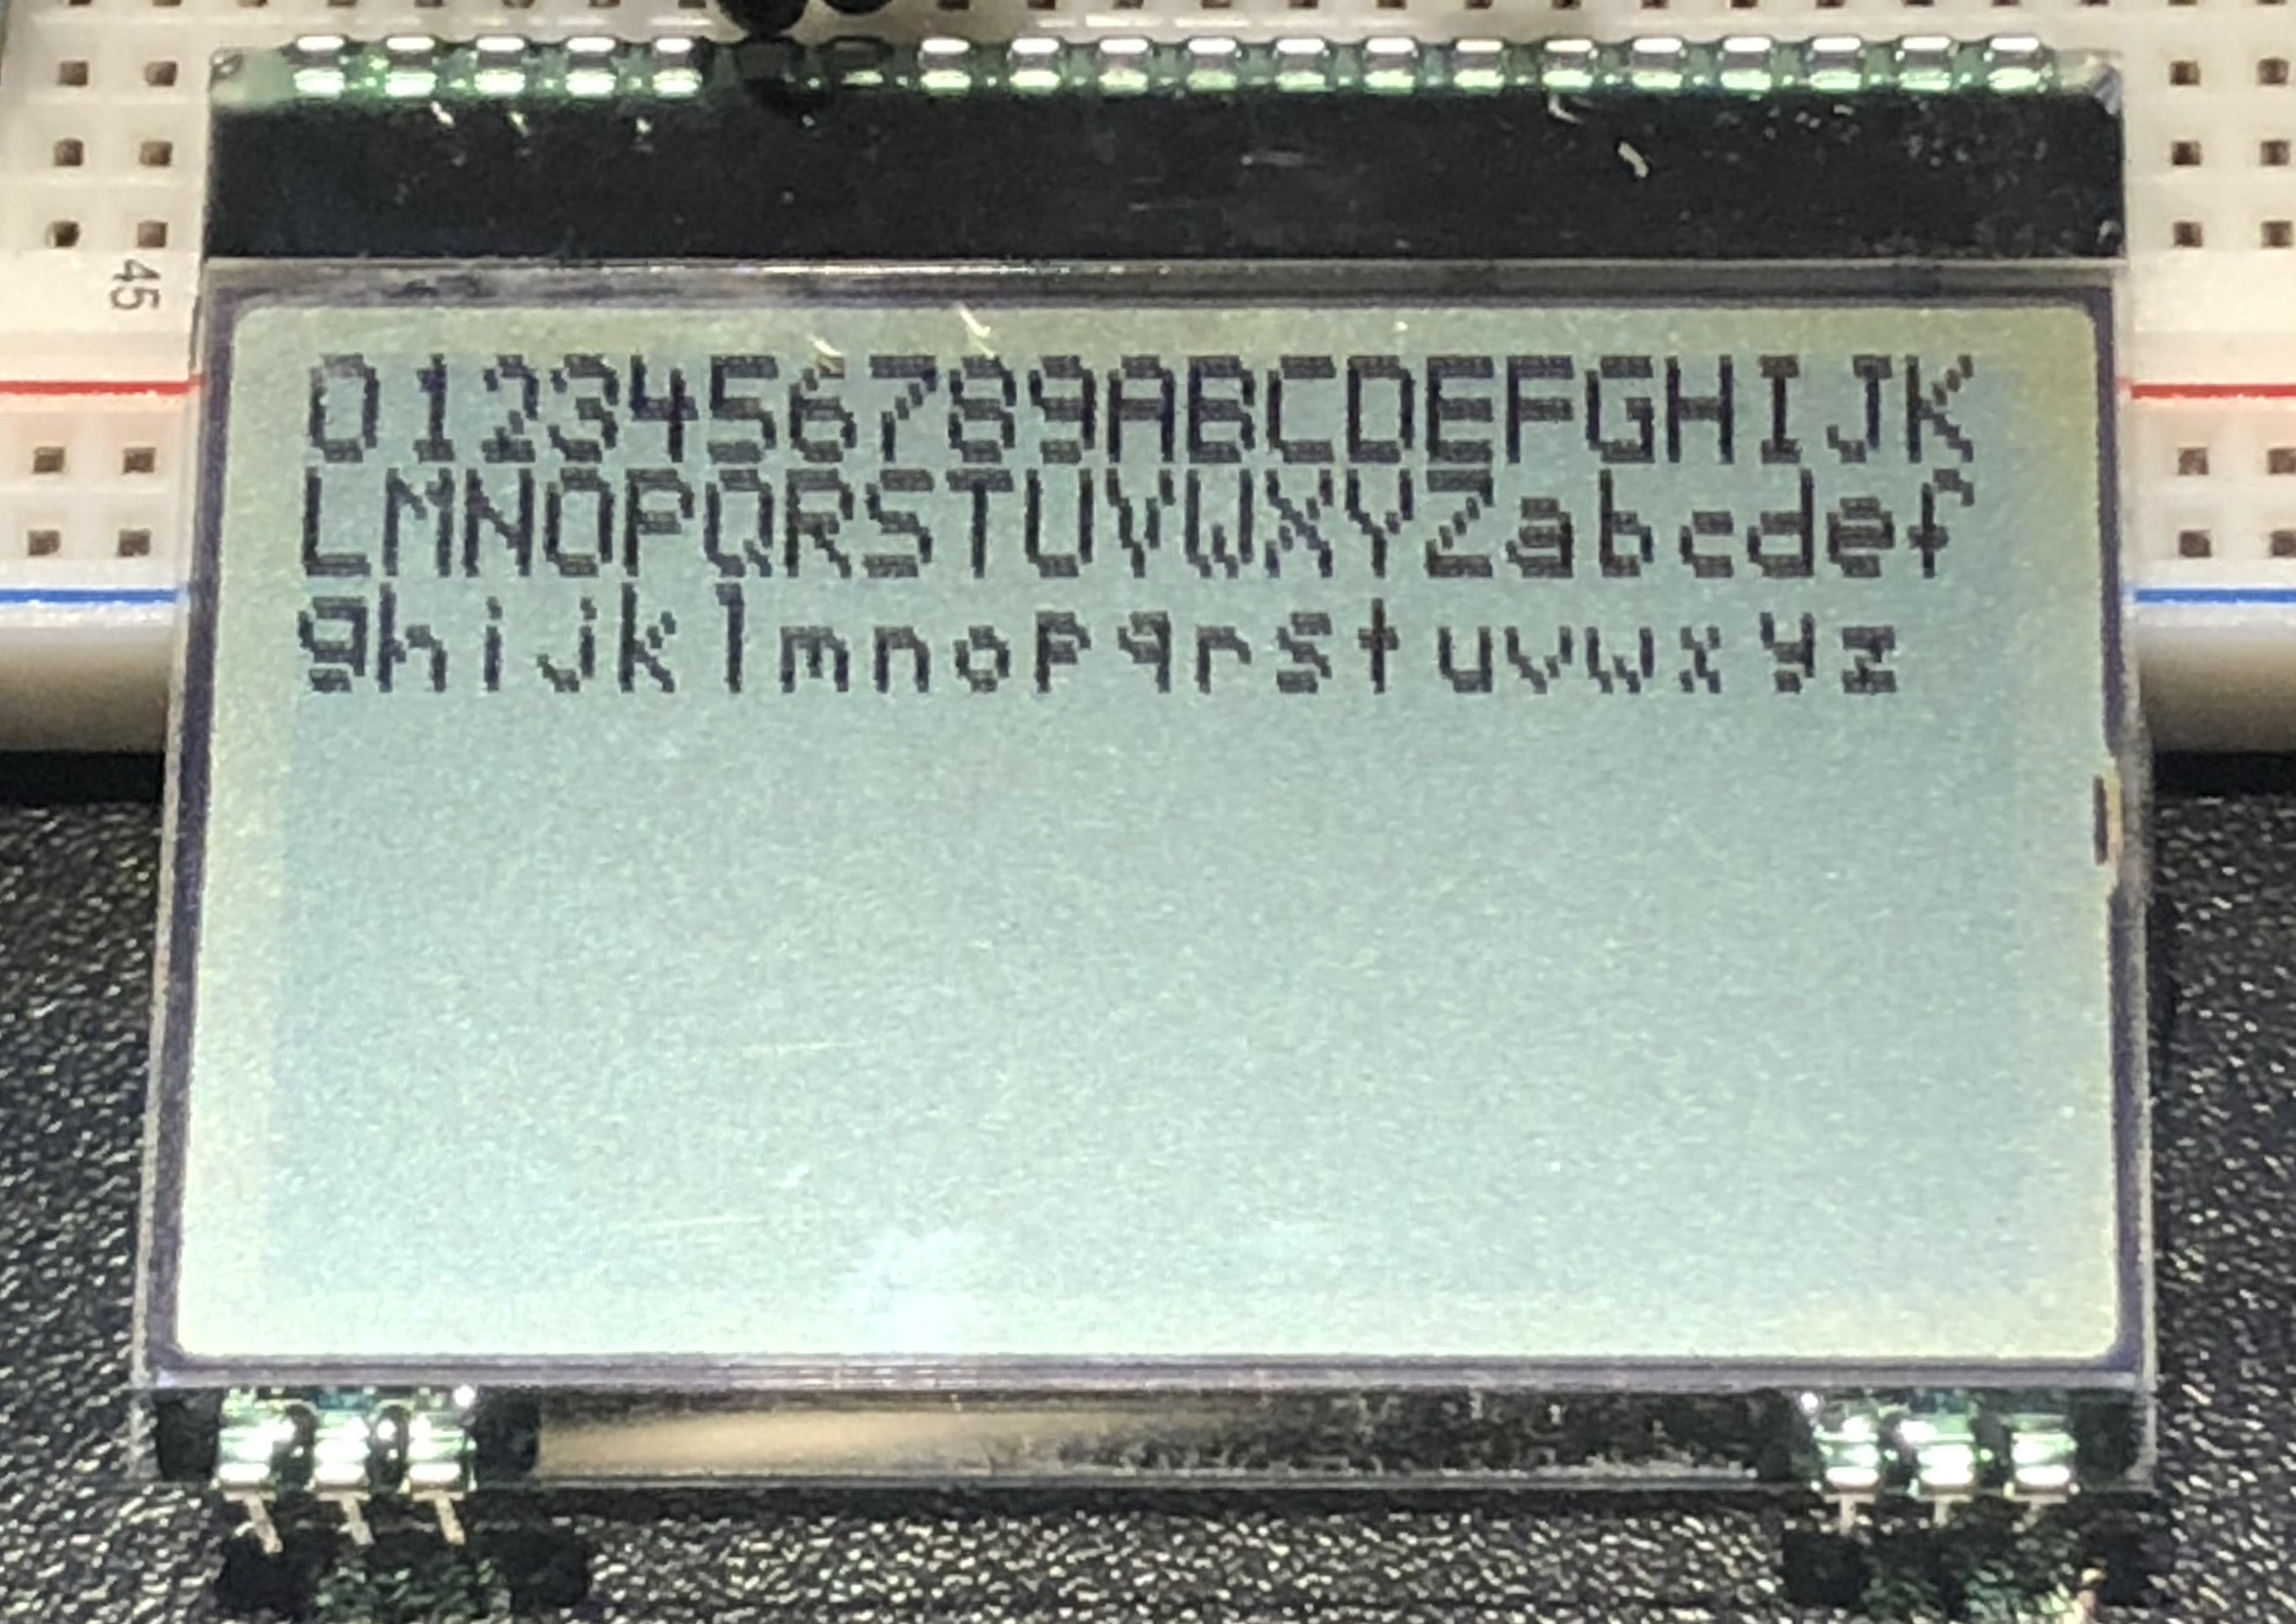
\includegraphics[width=0.3\linewidth]{assets/dogm128.jpg}
\caption{Das Display DOGM128W-6 auf einer Steckplatine.}
\label{fig:dogm_demo}
\end{figure}
\subsubsection{Knöpfe}
Als ich mir zum ersten Mal Gedanken darüber machte, welche Art Knöpfe ich benutzen soll, nahm ich meinen Schultaschenrechner auseinander und sah, dass die Plastikknöpfe auf eine Plastikmembran drücken, die eine Strombrücke auf dem PCB bildeten, wenn sie heruntergedrückt waren. Diese Membran herstellen lassen ist für ein Produkt, von dem es nur sehr wenige Endprodukte geben wird, nicht realisierbar. Also musste ich auf ganz normale Tastschalter zurückgreifen.
\\[\medskipamount]
Auch wenn ich eine grosse Auswahl auf \url{https://digikey.ch} vorfand, war der Auswahlprozess ziemlich leicht. Ich wollte nämlich Knöpfe, auf die man eine Plastikkappe aufsetzen und somit die Knöpfe beschriften kann. Nachdem ich nach diesen Merkmalen filterte, sortierte ich nach aufsteigendem Preis und nahm die günstigsten Knöpfe. Diese sind in Abbildung \ref{fig:button_image} zu sehen. Schlussendlich brauchte ich diese Plastikkappen eigentlich gar nicht, weil ich mit dem 3D-Drucker ein Knopffeld drucken konnte, dass ich einfach auf das Knopfgitter legen konnte.
\begin{figure}[H]
\centering
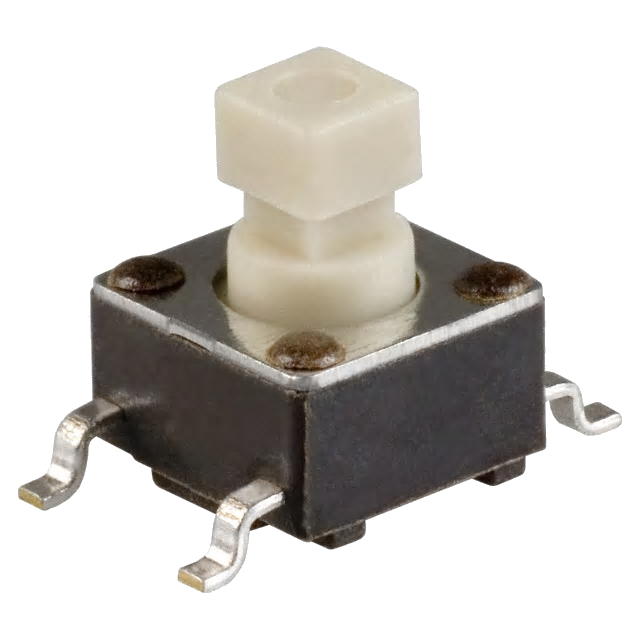
\includegraphics[width=0.2\linewidth]{assets/TL3301SPF260QG.png}
\caption{Der Tastschalter TL3301SPF260QG.}
\label{fig:button_image}
\end{figure}
\subsection{Prototyping}
Auf mehreren Steckplatinen platzierte ich Komponenten wie Display und Knöpfe und verband sie miteinander. Abbildung \ref{fig:prototyping} zeigt den letzten Stand des Prototyps, bevor ich das PCB bestellte. Man sieht auf der rechten Hälfte zuoberst den Arduino UNO, der alles steuert. Die neun blauen Komponenten sind 1$\mu$F-Kondensatoren, die zum Betrieb des Displays notwendig sind. Unter dem Display ist links der EEPROM zu sehen, der die Schriftart und Grafiken abspeichert. Auf der linken Steckplatine stecken zehn Tastschalter, die von einem Streifen Papier abgedeckt sind, der die Funktion der Knöpfe anzeigt. Die Sekundärfunktionen der Tasten, die blau auf dem Papierstreifen abgebildet sind, konnte man mit Druck auf den Knopf rechts unter dem Display aktivieren.
\begin{figure}[H]
\centering
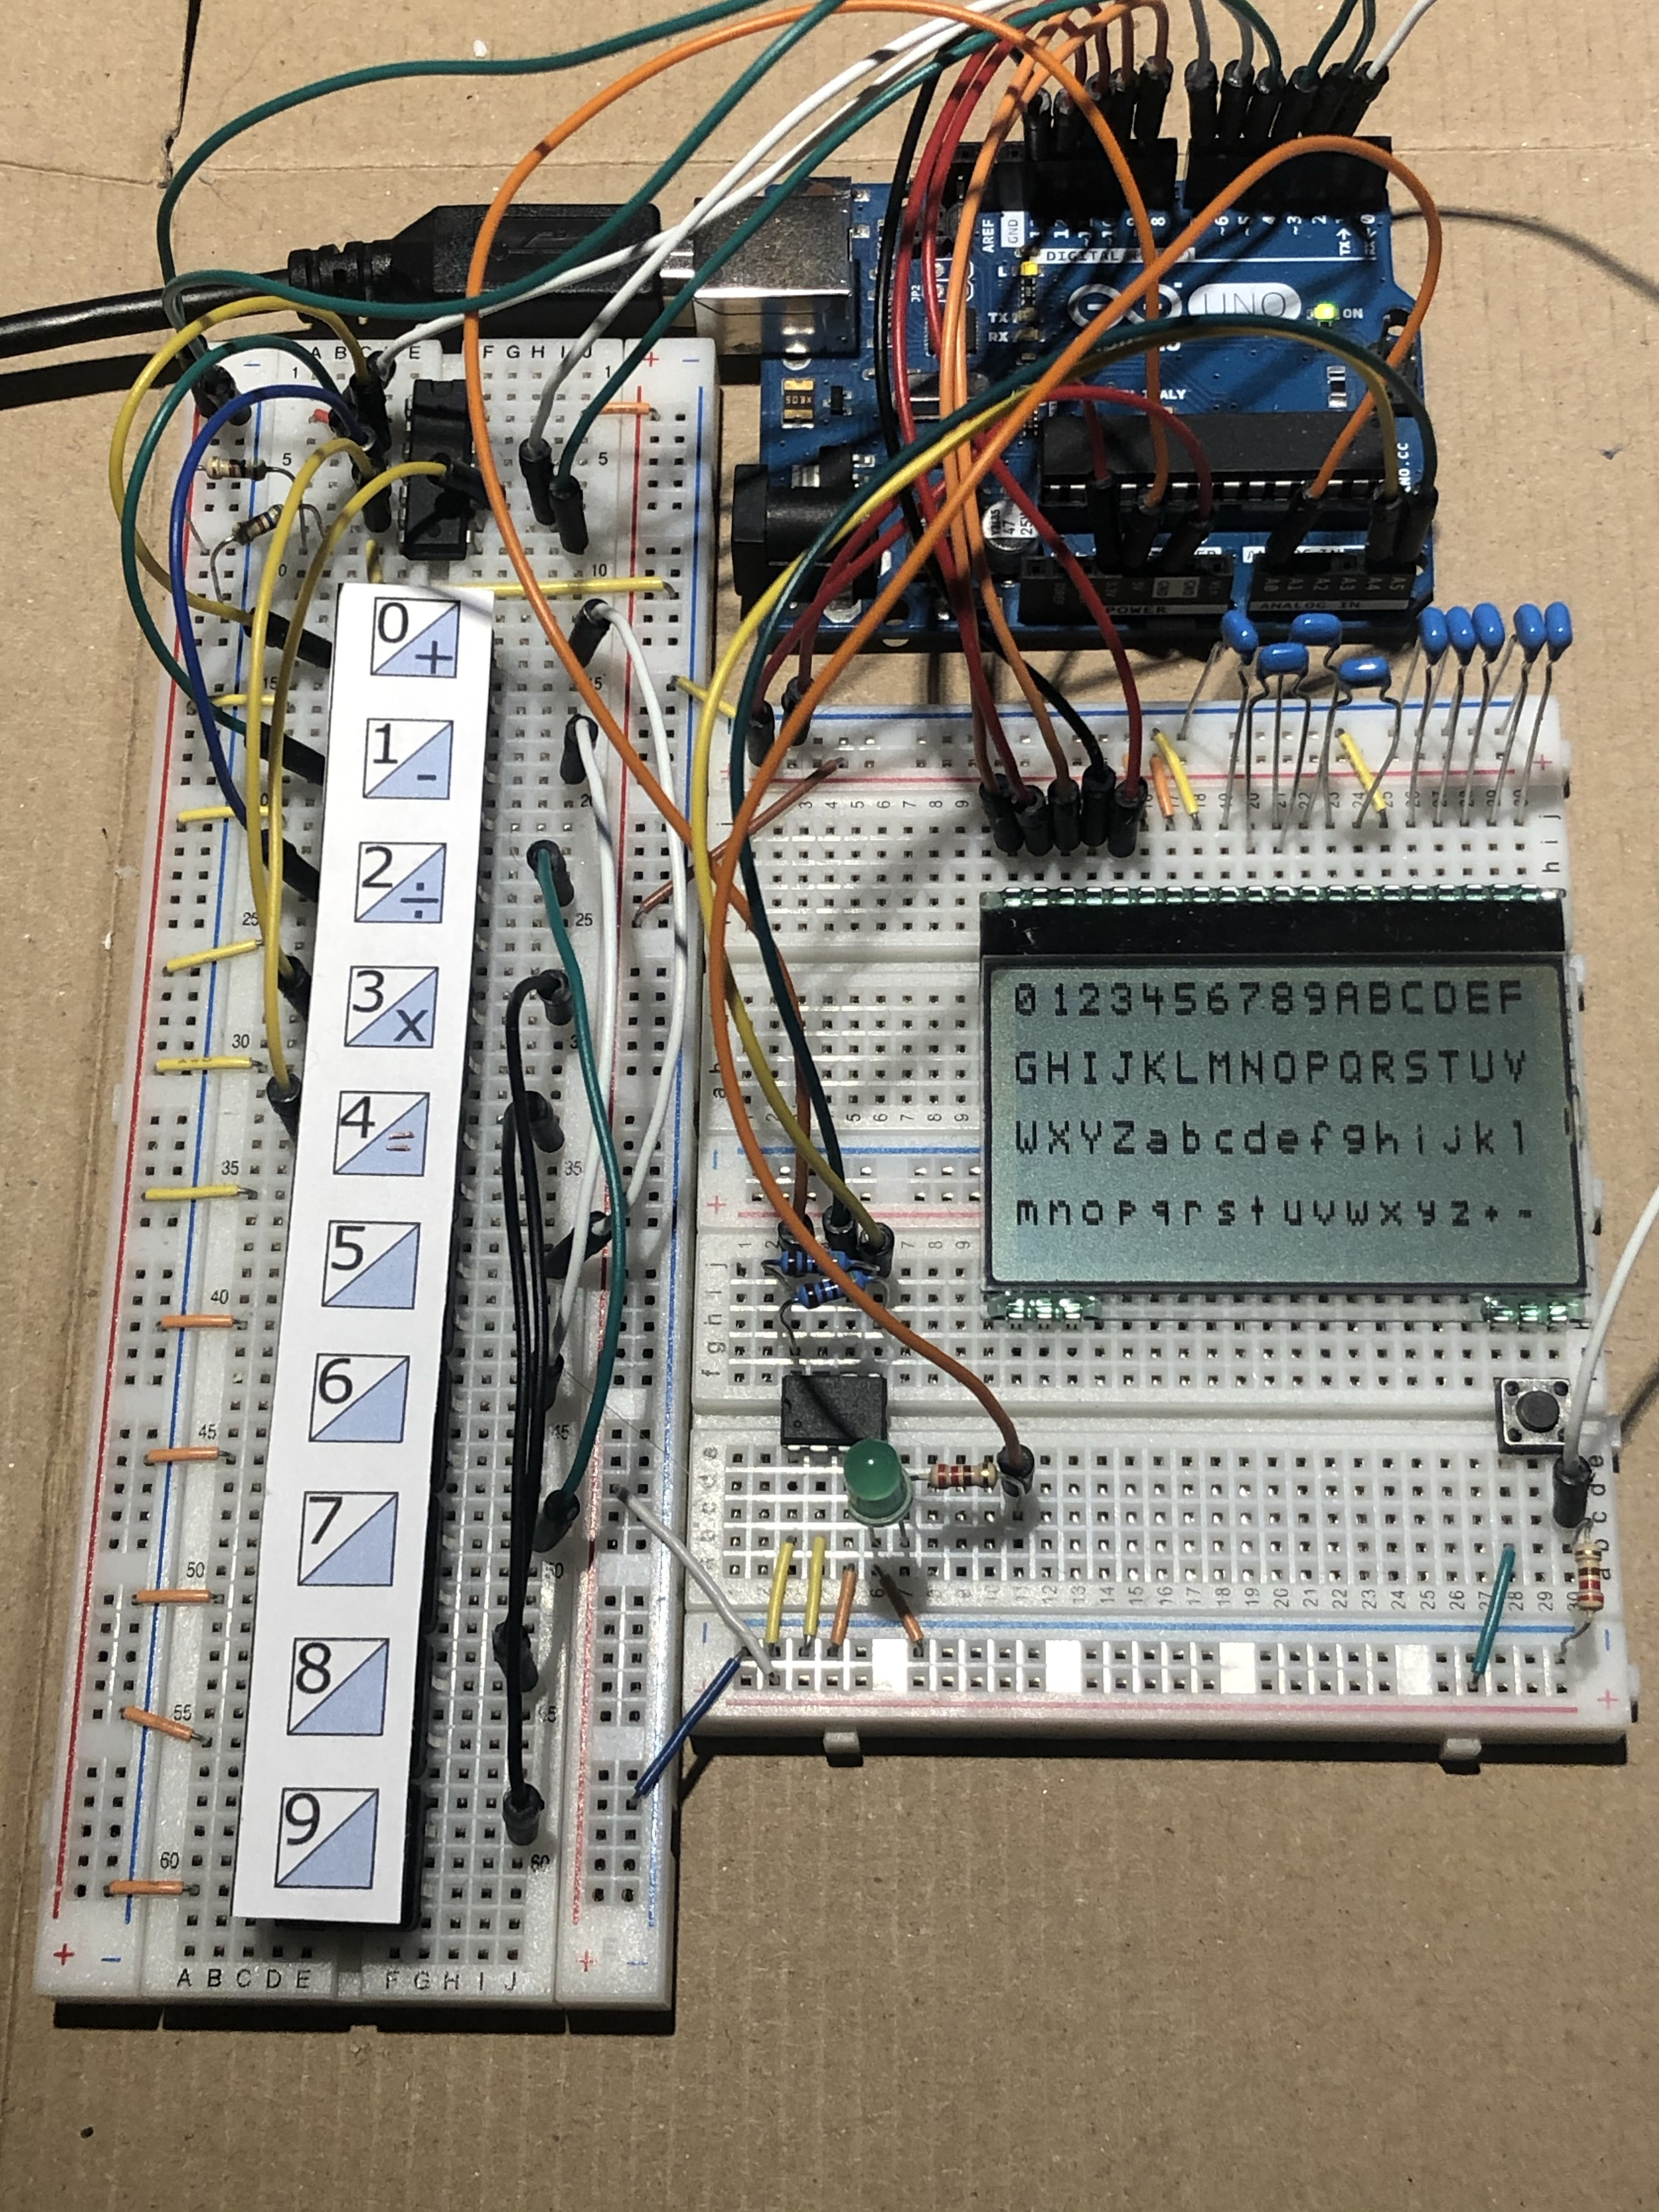
\includegraphics[width=0.6\linewidth]{assets/prototype.jpg}
\caption{Der letzte Prototyp auf Breadboards.}
\label{fig:prototyping}
\end{figure}
\subsection{Design des PCBs}
Im Mai begann ich mit der Suche nach Programmen, mit denen PCBs erstellt werden können. Als Erstes stiess ich auf EasyEDA, eine Web-Applikation, die eine grosse Auswahl an Komponenten schon integriert hatte, weil man als Benutzer Komponenten, die noch nicht auf der Seite verfügbar sind, erstellen und hochladen kann. Persönlich gefiel mir das Interface nicht wirklich, daher suchte ich weiter, nachdem ich mich eine Weile mit EasyEDA auseinander gesetzt hatte.
\\[\medskipamount]
Ich probierte als Zweites Autodesk EAGLE aus. Die reguläre Version der Software ist in dem Fusion 360-Abonnement inbegriffen\footnote{siehe \url{https://www.autodesk.com/products/eagle/free-download} (Abgerufen 13.10.2020)} und somit kostenpflichtig, aber es wird eine Version für den kostenlosen Gebrauch angeboten, die bestimmte Limitationen hat. Unter anderem ist die PCB-Grösse auf $80\textrm{cm}^2$ beschränkt, was ich aber vorerst nicht bemerkte, weil zu Beginn noch eine 30-tägige Testversion aktiv war. Das Display musste mindestens eine Breite von 60mm einnehmen, also hätte die Länge unter 135mm sein müssen, worauf ich kaum alle geplanten Komponenten hätte plazieren können. Somit sah ich mich gezwungen, erneut das Programm zu wechseln. Ich entschied mich für KiCad, eine Open-Source-Software.
\\[\medskipamount]
\begin{figure}[H]
	\centering
	\frame{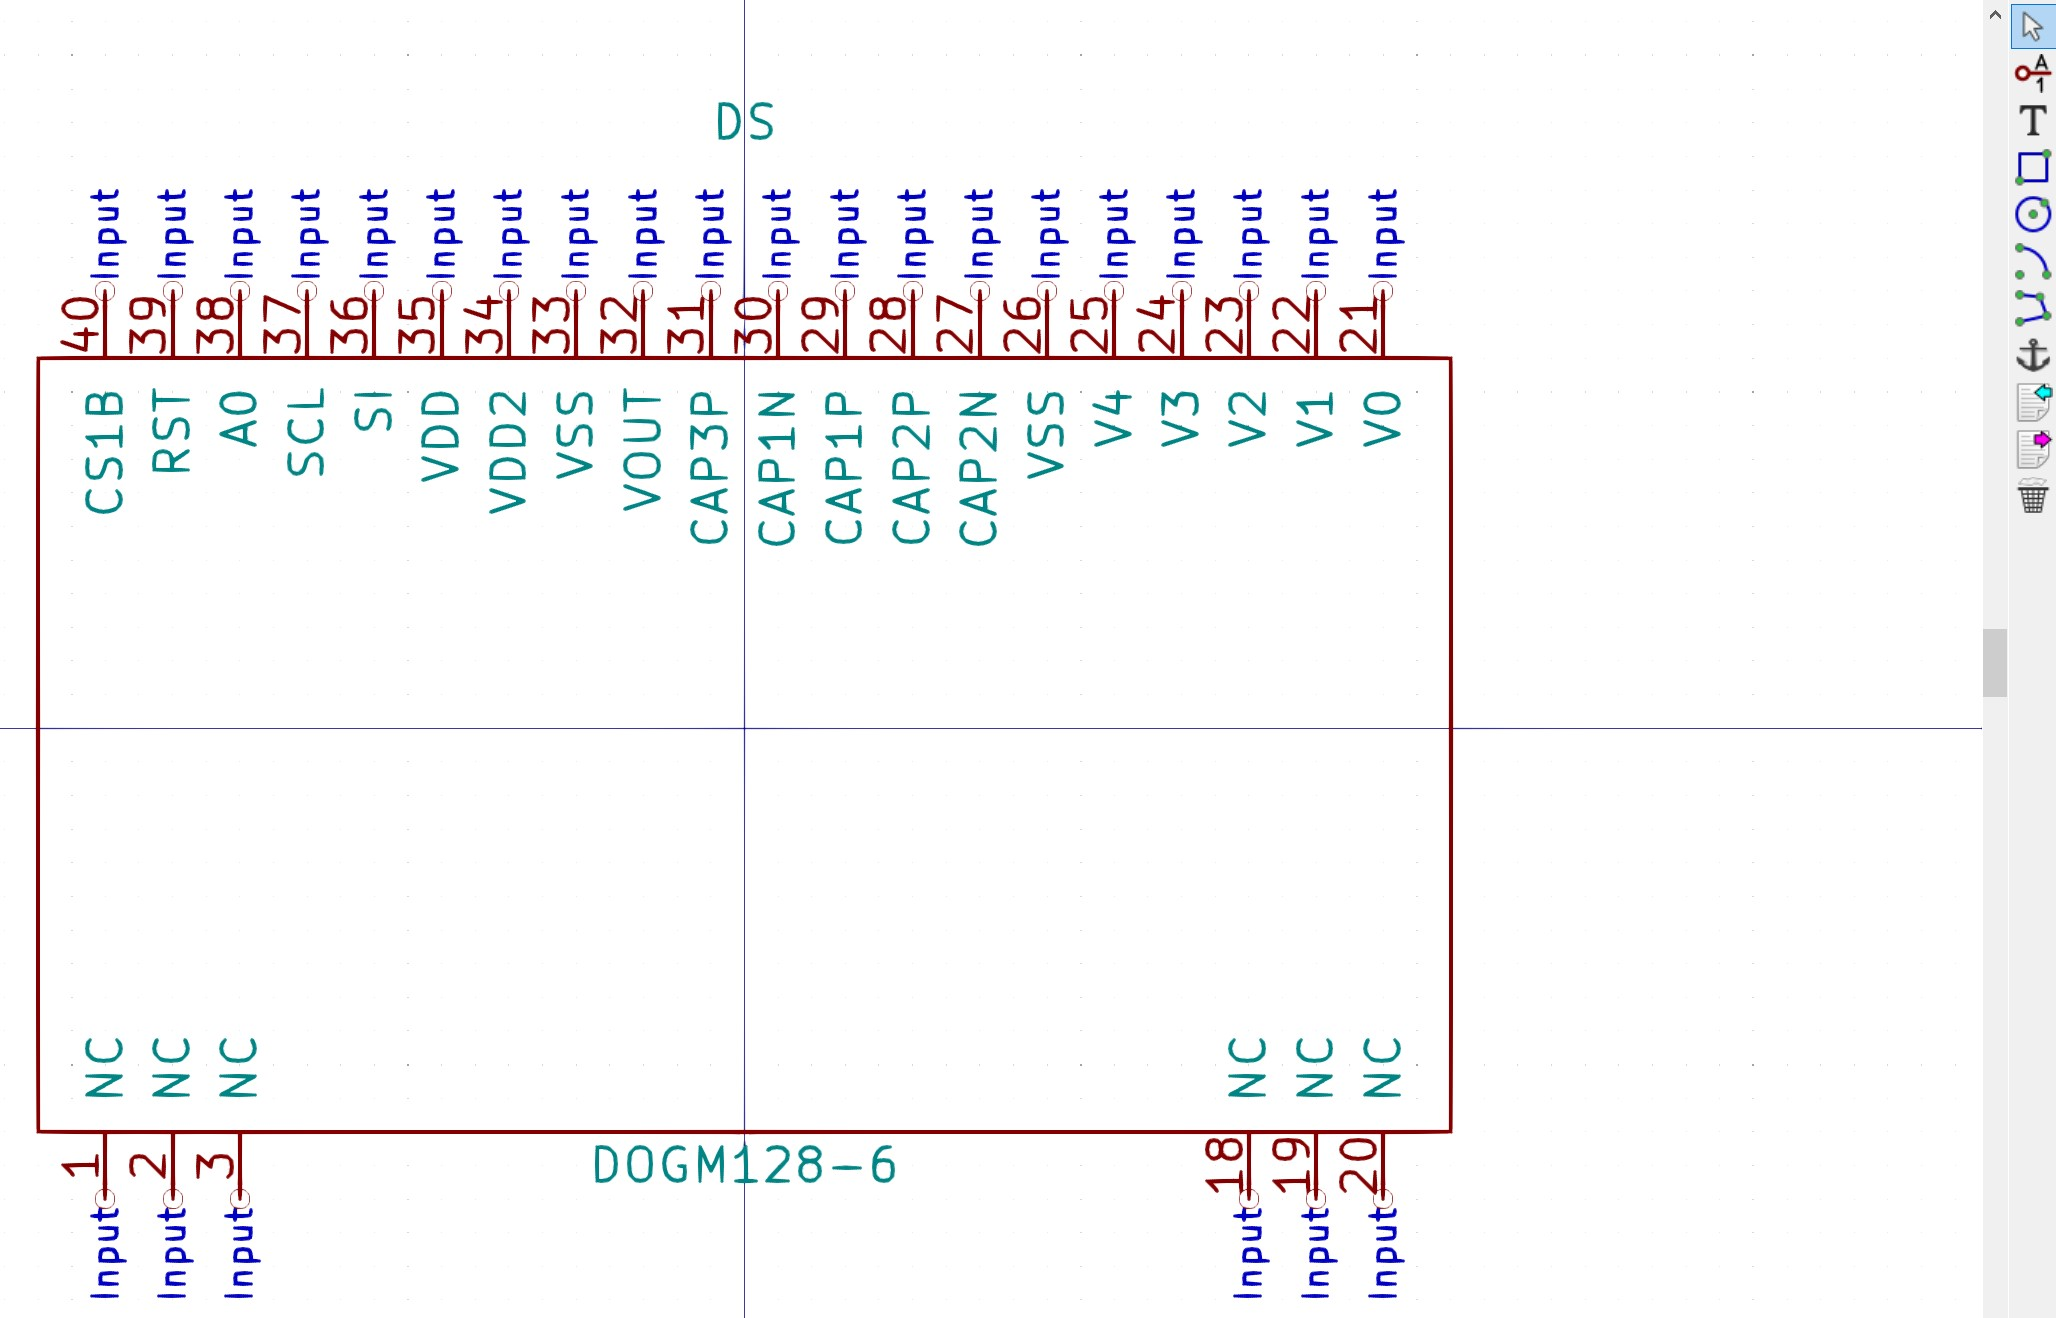
\includegraphics[width=\linewidth]{assets/symboleditor.jpg}}
	\caption{Der Symboleditor in KiCad.}
	\label{fig:symboleditor}
\end{figure}
In KiCad war das Display, dass ich benutzen wollte, das DOGM128W-6 von Electronic Assembly, nicht in der Footprint-Bibliothek vorhanden. Ich musste daher das Symbol für das Schema und den Footprint selbst erstellen. Ich begann mit dem Symbol und erstellte ein Rechteck, wo ich die Pins einsetzte, beschriftete und durchnummerierte (siehe Abbildung \ref{fig:symboleditor}). Für den Footprint gab es wesentlich mehr Arbeit, weil die Maschinen, die das PCB herstellen, wissen müssen, wo die Löcher für die Pins genau sind. Ich musste also die genauen Dimensionen und Abstände mit dem Datasheet des Displays herausfinden. Danach konnte ich anhand dieser Messungen im Programm den Footprint entwerfen. Ich druckte das PCB-Layout auf Papier aus und legte das Display darauf und konnte so verifizieren, dass die Dimensionen korrekt waren.
\subsection{Erster Prototyp auf PCB}
Das PCB bestellte ich bei einer chinesischer PCB-Fabrik namens JLCPCB. Es gibt zwar Möglichkeiten, PCBs in Europa herstellen lassen, aber die Preise sind viel günstiger bei den chinesischen Angeboten. Zum Vergleich: Der Preis, fünf meiner Taschenrechner-PCBs bei JLCPCB zu bestellen, ist 23.30 CHF mit Versandkosten\footnote{siehe \url{https://jlcpcb.com/} (Aufgerufen 17.10.2020)}. Bei Eurocircuits kosten fünf PCBs hingegen 112 CHF\footnote{siehe \url{https://www.eurocircuits.com/} (Aufgerufen 17.10.2020)}, was keineswegs ein Ausnahmefall ist.
\\[\medskipamount]
Anfangs Juli kam das bestellte PCB an. Weil die meisten Komponenten SMD-ICs waren, wäre es sehr mühsam gewesen, diese mit einem gewöhnlichen Löteisen anzulöten. Stattdessen kaufte ich eine SMD Reworkstation, eine Art Heissluftföhn, dessen Temperatur präzis eingestellt werden kann. Um mit der Reworkstation die Komponenten anlöten, muss zuerst auf die Kontakte Lötpaste gestrichen werden. Diese besteht aus kleinen Bällchen Lötzinn gemischt mit Flussmittel, die mit Hitze zusammenschmelzen und zwischen den Komponenten und den Pads eine elektrische Verbindung bilden\footnote{vgl. RS Components GmbH: Lötpasten.}. Aber auch mit diesen Hilfsmitteln hatte ich grosse Schwierigkeiten, die kleinen SMD-Komponenten wie den Mikrocontroller anzulöten. Entweder gab ich zu viel Lötpaste auf die Pads und mehrere Pins verbanden sich miteinander; es bildeten sich sogenannte Brücken, oder ich benutzte zu wenig Lötpaste und es bildete sich keine Verbindung zwischen den Pins und Pads.
\\[\medskipamount]
Als dann die ICs, das Display und etwa die Hälfte der Knöpfe angelötet waren, versuchte ich, mit dem Mikrocontroller über den Arduino UNO zu kommunizieren, ihn zu programmieren und das Display und die Knöpfe anzusteuern. Leider musste ich unzählige Male den Chip ab- und wieder anlöten und auf Lötbrücken testen, bis ich nach ein paar Tagen einen ersten Erfolg hatte und der Arduino den ATmega1284 erkannte.
\\[\medskipamount]
Das Mühsamste an der Fehlersuche während dieser Zeitspanne, wo ich versuchte, den PCB-Prototyp zum Laufen zu bringen, war die Unsicherheit, ob es sich um ein Software- oder Hardwareproblem handelte. Ich rechnete zwar meistens damit, dass es ein Hardwareproblem war, aber einige tückische Programmierfehler schlichen sich von Zeit zu Zeit ein, die ich lange übersah, weil ich an der Hardware nach Fehlern suchte. Wie sich schlussendlich herausstellte, gab es zwei grosse Fehler am PCB-Prototypen:
\begin{enumerate}
	\item Ich hatte bei den Knöpfen falsch verstanden, welche Pins immer verbunden sind und welche nur bei Knopfdruck Strom durchfliessen lassen. Dies führte dazu, dass der Mikrocontroller immer alle Knöpfe als gedrückt sah.
	\item Das Grundpotenzial des Akkus floss nicht zu allen Komponenten, sondern nur zum Grundpotenzial des Auflade-ICs. Somit konnte der Akku dem Taschenrechner keinen Strom liefern.
\end{enumerate}
Den ersten Fehler konnte ich temporär beheben, indem ich die Knöpfe um 30 Grad drehte, sodass die Pads, zwischen denen Strom bei Knopfdruck fliessen soll, mit den Pins der Knöpfe, die tatsächlich nur bei Knopfdruck Strom leiten, verbunden sind.
Das zweite Problem liess sich nicht so einfach umgehen und ich musste auf eine zweite Version des PCBs warten. Weil aber der Arduino UNO über die Programmierpins auch Strom liefert, konnte ich trotzdem am Taschenrechner arbeiten.
\subsection{Zweiter Prototyp auf PCB} \label{secondproto}
In KiCad behob ich die beiden erwähnten Probleme. Zusätzlich fügte ich neben dem USB-Port noch vier Pins hinzu, die von links nach rechts an die GND-, TXD-, RXD- und 5V-Pins der Mikrocontollers angeschlossen sind. Mit diesen Pins war es möglich, Sensoren oder andere Erweiterungen anschliessen. Der Plan war, mit dem Taschenrechner eine erste Anwendung zu finden auf einer Gletscherexkursion, wo mit einem angeschlossenen Barometer-Sensor die aktuelle Höhe berechnet werden konnte (Mehr dazu im Kapitel \ref{excursion}). Ich bestellte das neue PCB, sowie die Komponenten ein zweites Mal. Dieses Mal schien alles zu klappen und auch der Akku konnte dem Taschenrechner Strom liefern. Als ich dann aber versuchte, den Taschenrechner über den USB-Port aufzuladen, stieg die Spannung des Akkus, die ich mit einem Multimeter mass, nicht. Grund war, dass der 0V-Pin des Auflade-ICs zum 0V-Pin des USB-Ports ging und nicht zum Minuspol des Akkus. Dieses Problem konnte ich zum Glück mit einem Kabel, dass von einem 0V-Pin auf dem Taschenrechner zu dem 0V-Pin des USB-Ports ging (in Abbildung \ref{fig:calcview} zu sehen), lösen. Ausser diesem Fehler gab es keine anderen Hardwareprobleme.
\subsection{Programmentwicklung}
Das Programm ``Visual Studio Code'' von Microsoft ist eine Programmierumgebung, die aber nicht speziell für eine spezifische Programmiersprache entwickelt wurde, sondern eher ein Code-Editor ist, der mit Erweiterungen für viele Programmiersprachen Unterstützung bietet. Es enthält ein Dateibrowser, Git-Integrierung und vieles mehr.
\subsection{Benennung des Taschenrechners}
Als es an der Zeit war, ein Projekt auf GitHub, einer Version Control-Plattform, zu erstellen, musste ich mir einen Namen einfallen lassen. Nach nicht besonders langem Überlegen entschied ich mich, einen temporären Namen zu geben, den ich vorhatte, später abzuändern: CALCKS. Der Name stand für ``\textbf{Calc}ulator from a \textbf{K}ZO \textbf{s}tudent''. Schlussendlich nahm ich aber doch nie eine Namensänderung vor und der Name des Taschenrechners blieb bei CALCKS.
\subsection{Gehäuse}
Ich hatte mir schon seit einiger Zeit einen 3D-Drucker aus diversen Gründen kaufen wollen, und das Maturprojekt sah ich als einen guten Zeitpunkt, diesen Kauf zu tätigen, weil das Gehäuse mit einem 3D-Drucker gut herstellbar ist. Die Schwierigkeit bei der Wahl war, dass der Drucker eine genug grosse Druckfläche haben musste, aber trotzdem noch im meinem Budget von circa 300-400 Franken liegen sollte. Ich entschied mich schlussendlich für den Ender 3 Pro von Creality und kaufte dazu noch schwarzes PLA-Filament.
\\[\medskipamount]
Dies bedeutete, dass ich ein weiteres neues Programm für das Design von druckbaren 3D-Objekten erlernen musste. Das Programm Fusion 360 ist auch ein Autodesk-Produkt, aber zu diesem war eine Lizenz verfügbar, das für Schüler und Studenten die Basisversion des Programms gratis zur Verfügung stellt\footnote{siehe \url{https://www.autodesk.com/campaigns/education/fusion-360} (Abgerufen 16.10.2020)}. Wie ich später feststellte, hätte ich diese Lizenz auch für das Erstellen des PCBs brauchen können, aber weil das PCB zu dem Zeitpunkt schon fertig war, machte es keinen Sinn mehr, zurückzuwechseln.
\\[\medskipamount]
Auf alle Fälle begann ich mit dieser Software, das Gehäuse zu entwerfen. Ich versuchte als erstes, Knopfkappen mit Zahlen zu modellieren und zu drucken. Nach langem Experimentieren hatte ich zwar mehr oder weniger funktionsfähige Knopfkappen (siehe Abbildung \ref{fig:buttoncap}), aber ich realisierte, dass es mehr Sinn machen würde, einen sehr dünnen und somit flexiblem Boden mit herausragenden Knöpfen auszudrucken, weil dann weniger zusammengesteckt werden musste und ich mir keine Sorgen darüber machen musste, dass die Knopfkappen abfallen könnten.
\begin{figure}[H]
	\centering
	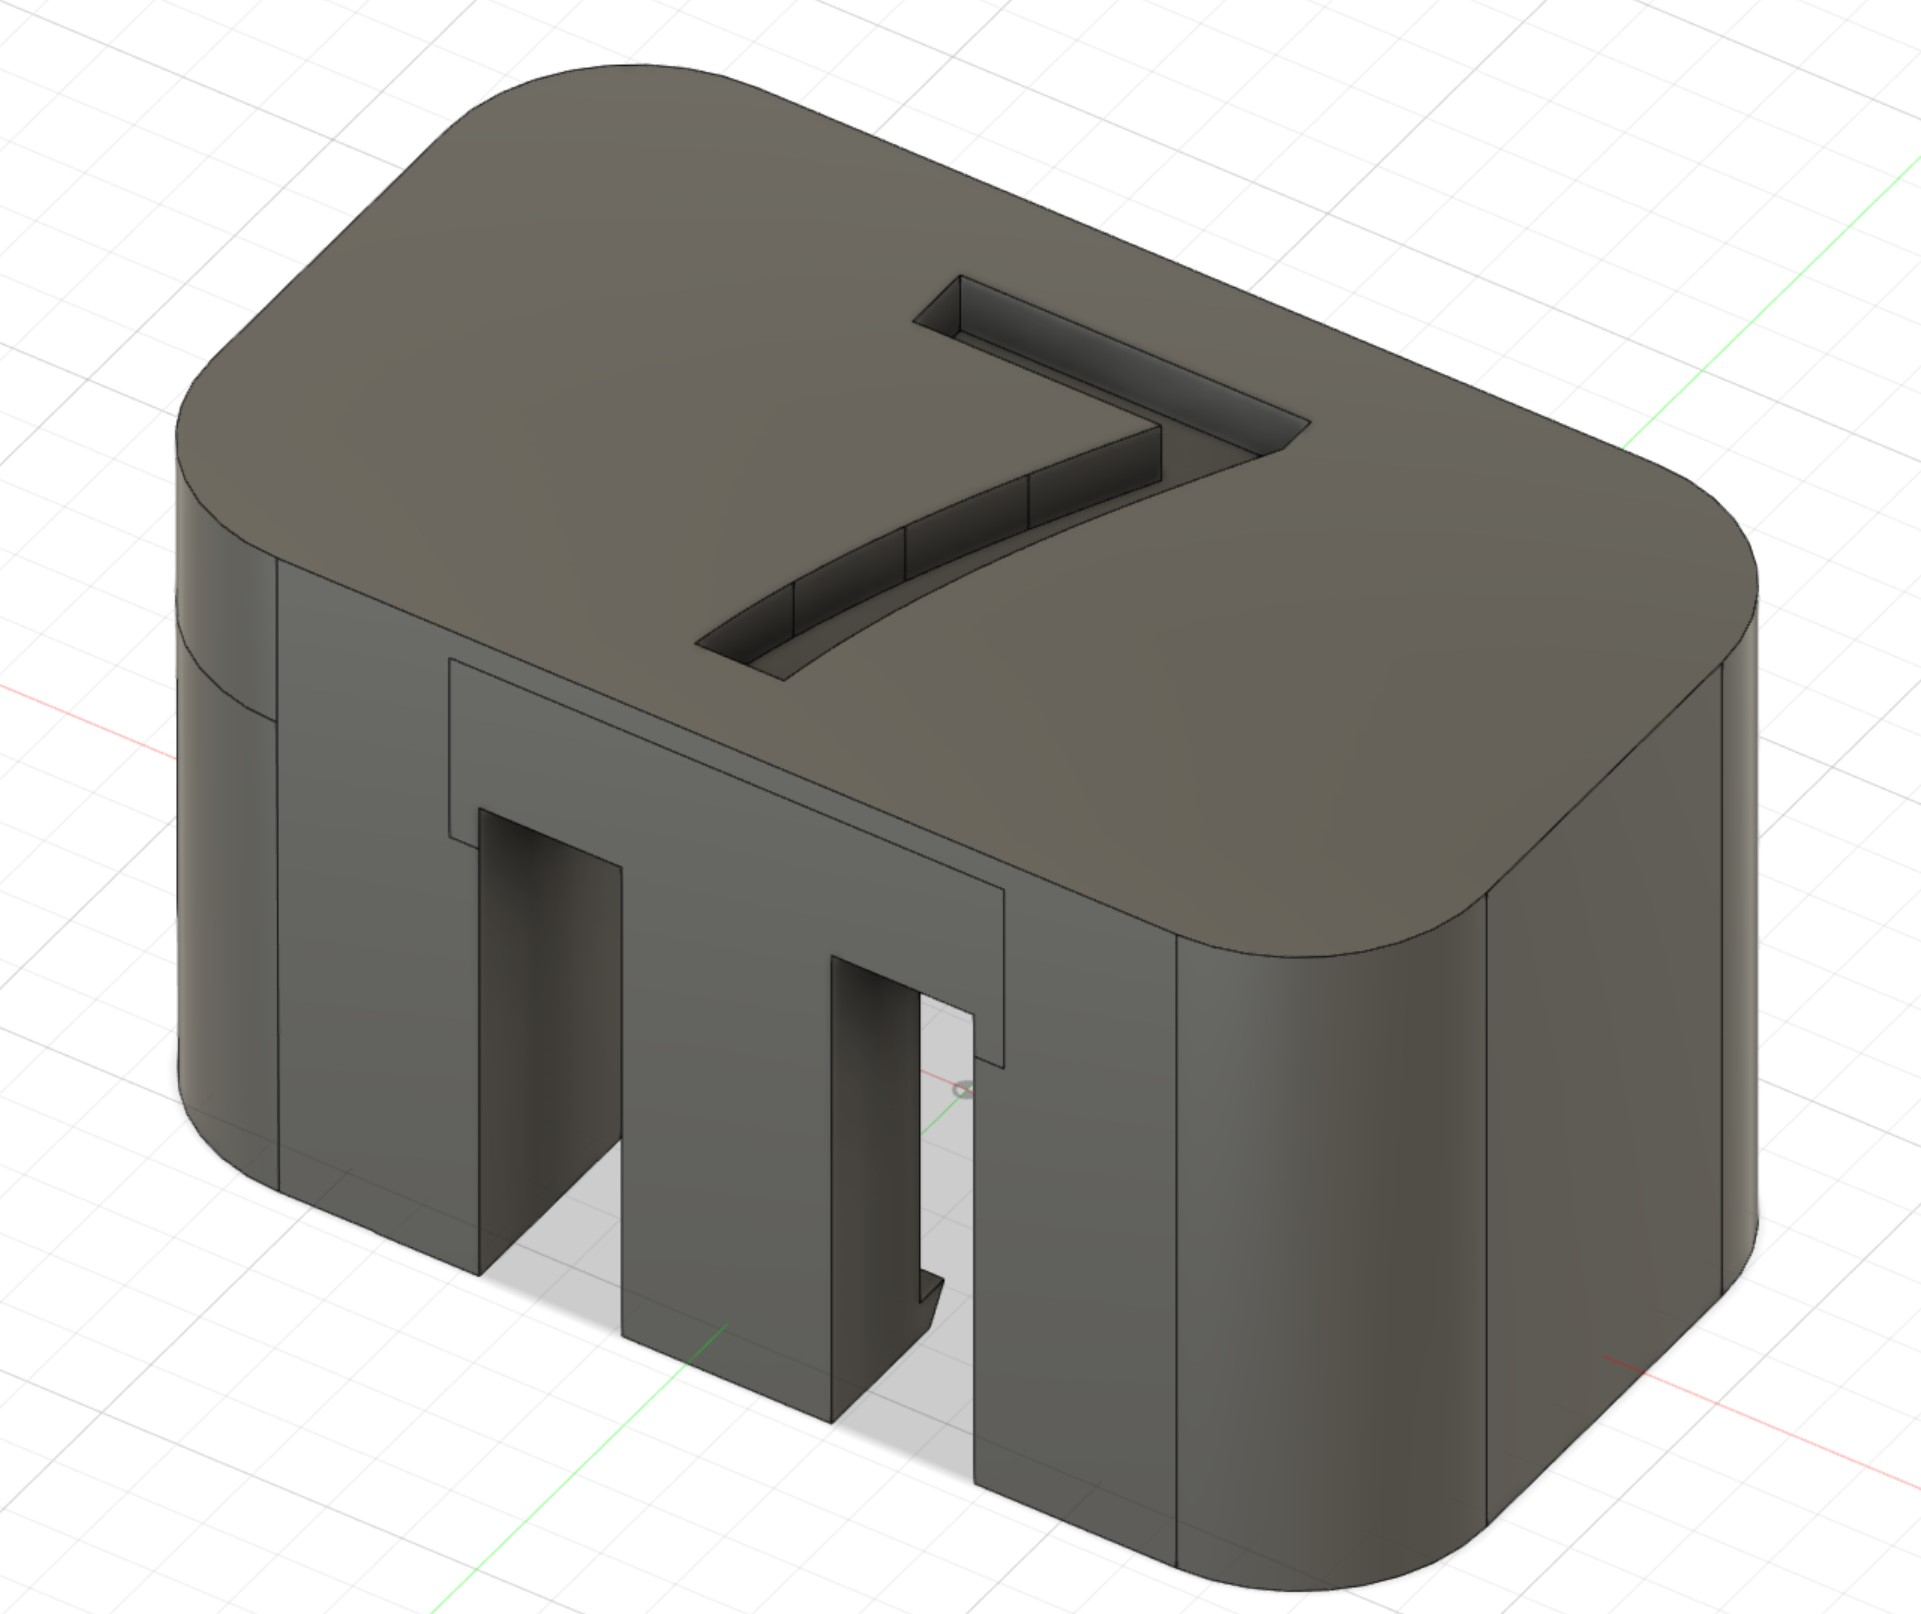
\includegraphics[width=0.3\linewidth]{assets/button7.jpg}
	\caption{Eine Knopfkappe, entworfen in Fusion 360.}
	\label{fig:buttoncap}
\end{figure}
\noindent
Auch das Design des Gehäuses erforderte viel Probierarbeit und Geduld, weil das Ausdrucken der Gehäuseteile zwei bis sieben Stunden dauerte. Aus diesem Grund konnte ich höchstens alle zwei Tage einen neuen Druck haben, weil ich dazwischen die Fehler beheben und dann auf den Druck warten musste.
\chapter{Technische Umsetzung}
\section{Hardware}
\subsection{Knopfmatrix}
Der ATmega1284 (im Packaging-Typ 44-TQFP) hat 44 Pins, von denen 32 Pins als Input/Output verwendet werden können\footnote{vgl. Microchip Technology: megaAVR® Data Sheet. 2020, S. 2.}. Der Taschenrechner hat aber 40 Knöpfe, also konnte ich nicht jeden einzelnen Knopf an einen Pin anschliessen. Stattdessen verwendete ich die folgende Methode:
\\[\medskipamount]
Die Knöpfe sind grundsätzlich, wie in Abbildung \ref{fig:buttonsgridschematic}, in einem 7x5-Gitter angeordnet, aber solange die Verbindungen gleich bleiben, können die tatsächlichen Positionen der Knöpfe willkürlich gesetzt werden. Bei diesem Gitter sind alle rechten Pins der Knöpfe jeder Spalte miteinander verbunden und führen zu den Pins des Mikrocontrollers (in der Abbildung: \textup{BTN\textunderscore ROW1--BTN\textunderscore ROW5}). Alle linken Pins der Knöpfe in einer Reihe sind miteinander verbunden und führen zu je einem Output-Pin des 8-Bit Serial-In-Parallel-Out Shiftregister-ICs (siehe Kapitel \ref{Shiftregister}) SN74HC164. Die vier Pins CLR, $\overline{\textrm{CLK}}$, A und B führen zu Pins des Mikrocontrollers. A und B werden intern im Shift-Register mit einem UND-Gatter kombiniert und haben die Funktion des Input-Pins, weshalb A und B zusammenführen und zum selben Pin am ATmega1284 führen.
\\[\medskipamount]
Will der Taschenrechner auf gedrückte Knöpfe überprüfen, sendet er einen Startpuls zum Shiftregister, was dazu führt, dass Strom durch die erste Reihe fliesst. Ist nun ein Knopf in dieser Reihe gedrückt, leitet der Knopf den Strom weiter, durch die Spalte, in welcher der Knopf ist. Der Mikrocontroller kann somit, falls ein Signal bei einem der fünf Reihen-Pins landet, genau wissen, welcher Knopf gedrückt ist. Danach betätigt der Mikrocontroller den CLK-Pin und der Strom fliesst durch die nächste Reihe. Der $\overline{\textrm{CLK}}$-Pin wird weitere fünf Male betätigt, bis er bei der letzten Reihe ankommt. Danach wird das Shiftregister über den CLR-Pin zurückgesetzt. Ein Problem entsteht hierbei: Der Mikrocontroller muss einen weiteren IC ansteuern, um die Zustände der Knöpfe auszulesen. Wenn aber der ATmega in den Schlafmodus geht, führt er auch keinen Code mehr aus. Das Aufwachen aus dem Power-down-Zustand kann er nur durch eine direkte Pinänderung oder eine Adressierung des Chips über das TWI-Modul\footnote{vgl. Microchip Technology: megaAVR® Data Sheet. 2020, S. 50.}.
\\[\medskipamount]
Aus diesem Grund enthält der Taschenrechner fünf zusätzliche Knöpfe, die direkt an den Mikrocontroller angeschlossen sind. Dies ist der Anschalteknopf und die vier Richtungsknöpfe.
\begin{figure}[H]
	\centering
	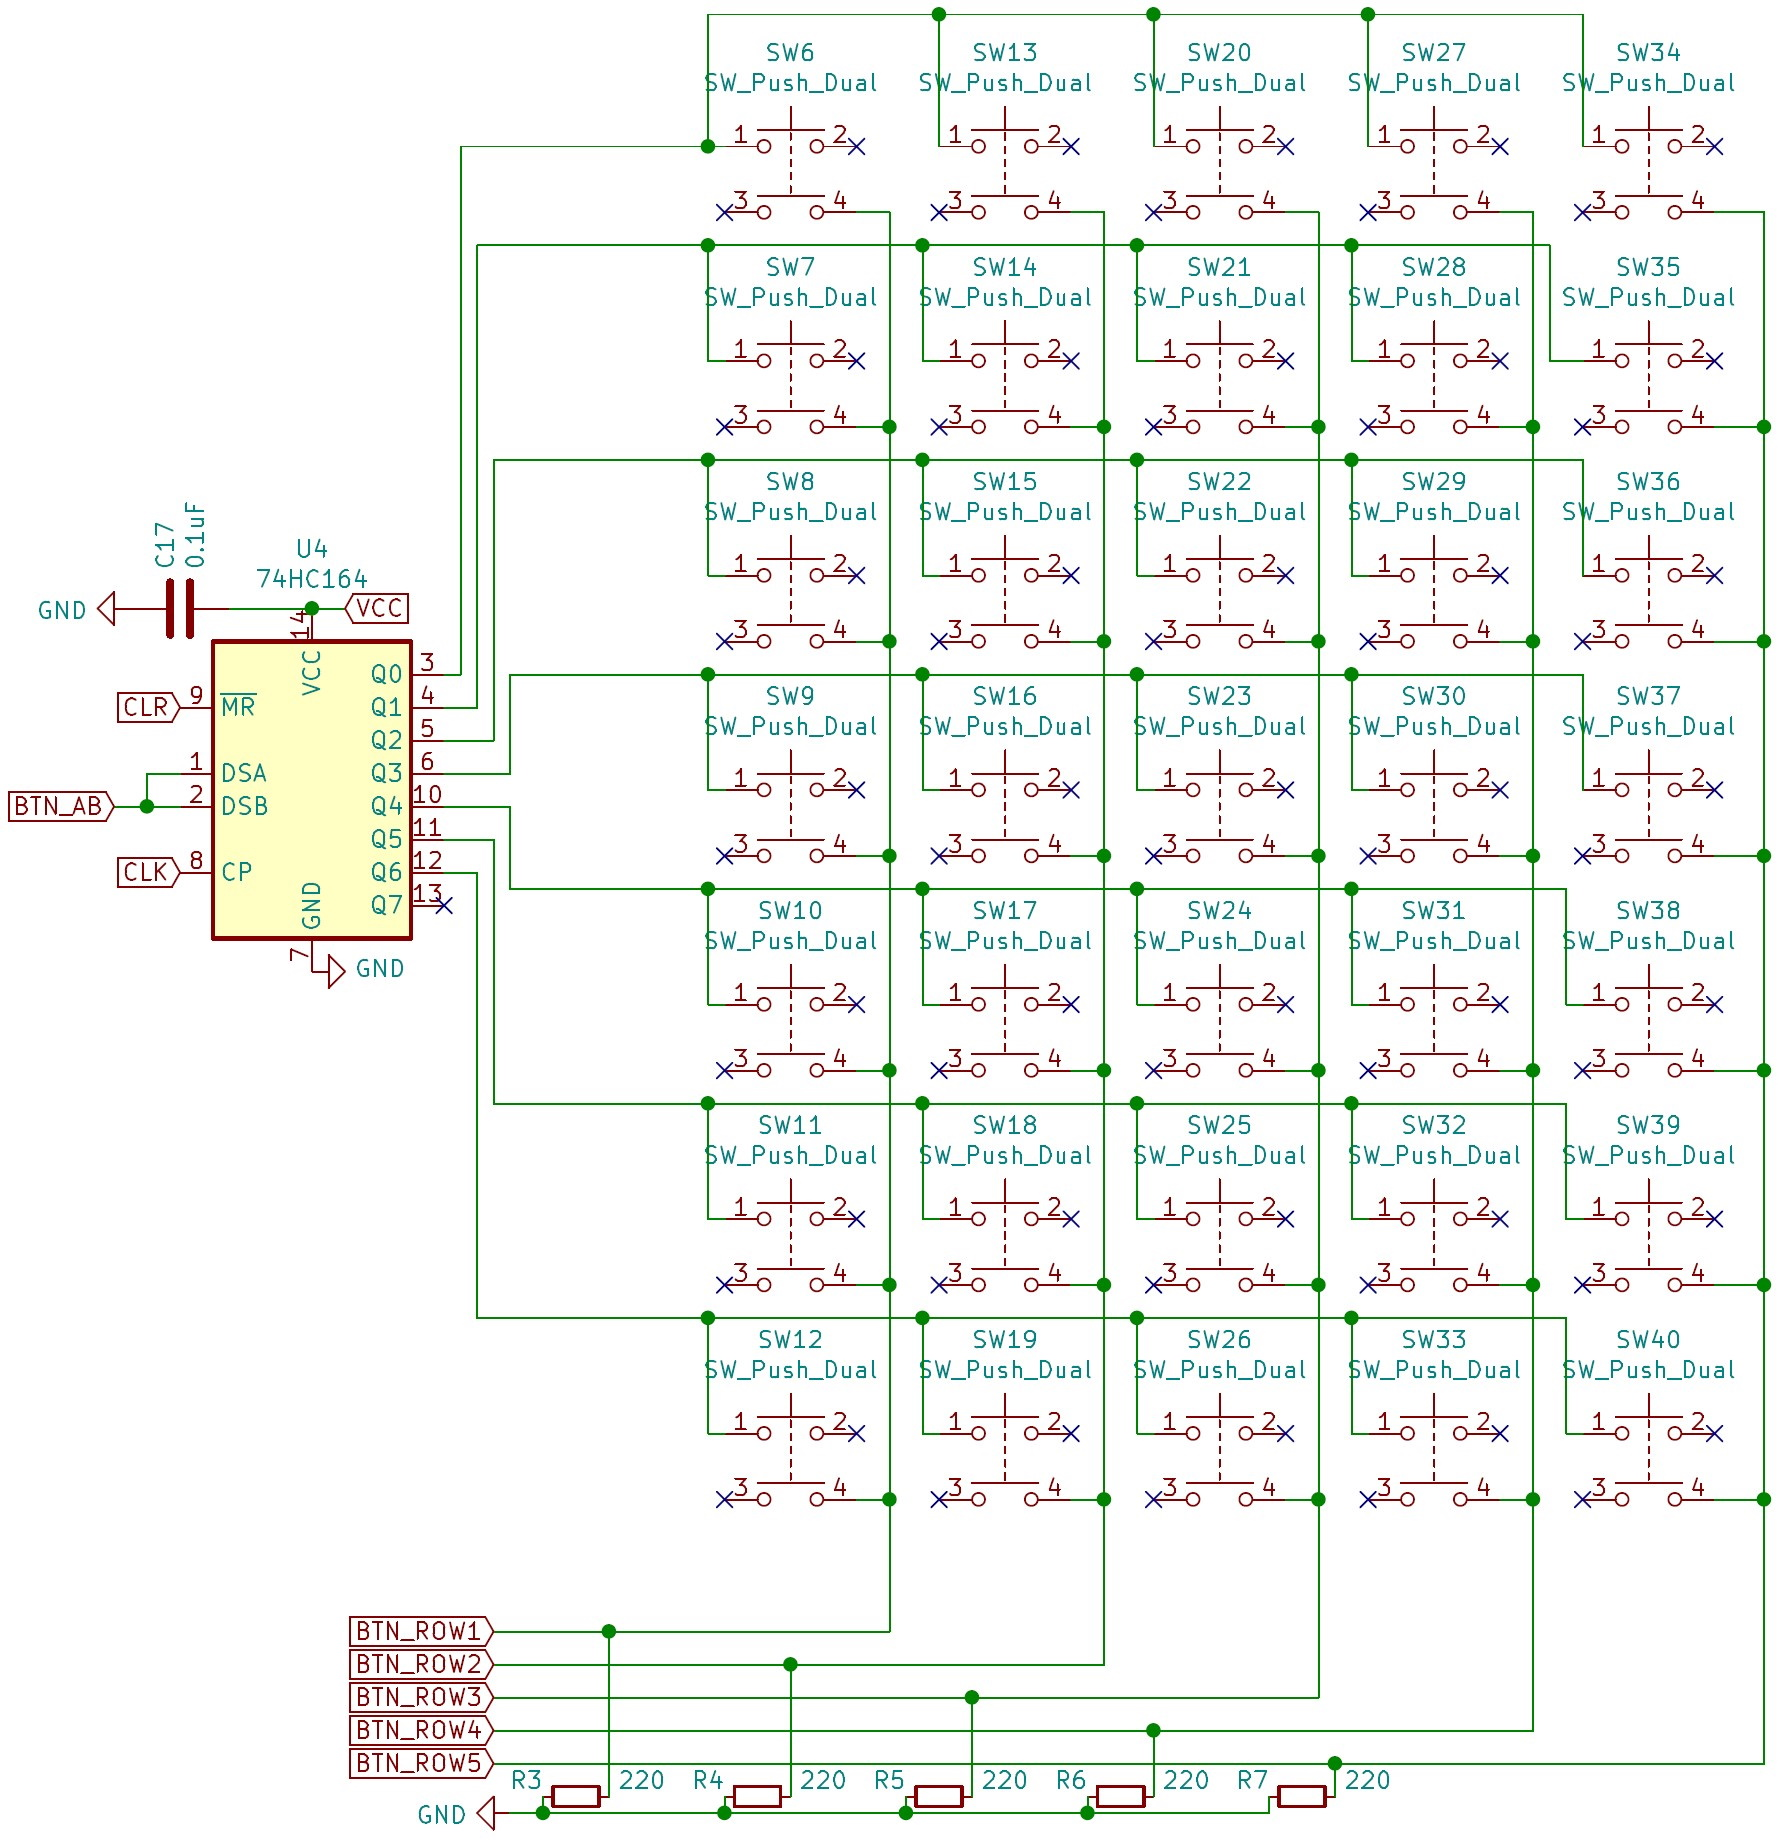
\includegraphics[width=\linewidth]{assets/screenshot_sc_buttons.jpg}
	\caption{Das Knopfgitter im Schema.}
	\label{fig:buttonsgridschematic}
\end{figure}
\subsection{PCB}
Das Schema und eine gerenderte Version des PCB-Layouts ist im Anhang vorzufinden.
\subsection{Stromversorgung}
Ich entschied mich schlussendlich, einen wiederaufladbaren Lithium-Polymer-Akku zu verwenden. Die benötigten Komponenten, damit der Akku dem Taschenrechner Strom liefern und wieder aufgeladen werden kann, sind die folgenden:
\begin{itemize}
	\item Ein IC, der die richtige Ladespannung generieren kann und automatisch beim Erreichen des aufgeladenen Zustands aufhört, Strom an den Akku zu übertragen.
	\item Ein Mikro-USB-Anschluss, damit der Taschenrechner über eine universelle Schnittstelle aufgeladen werden kann.
	\item Ein IC, der den Akku vor Tiefentladung schützt. Diesen könnte man theoretisch weglassen, aber wenn ein Akku unter der minimalen Spannung sinkt, reduziert dies die Lebensdauer des Akkus stark.
\end{itemize}
Der Akku ist ein Lithium-Polymer-Akku von Renata SA, der eine Nominalspannung von 3.7V und eine Nominalkapazität von 450mAh hat. Dieser Akku hat einen Schutzkreislauf bereits integriert, der ihn automatisch bei 3.0V ausschaltet.\footnote{vgl. Renata SA: Datasheet ICP582930PR-01. 2019, S. 1.}
\\[\medskipamount]
Für den Auslade-IC sah ich zwei Möglichkeiten. Ich hätte ein vorgefertigtes Akku-Auflade-PCB kaufen können, welches schon einen Mikro-USB Anschluss und 4 Lötpads hat, die zum Akku und zum Haupt-PCB führen. Die andere Möglichkeit war, einen Auflade-IC direkt auf dem PCB, wo alle anderen Komponenten darauf lagen, zu integrieren. Der Vorteil hier war, dass ich nicht ein zweites PCB in das Gehäuse montieren müsste. Der Nachteil war, dass ich so ein grösseres Risiko einginge, etwas im Schema falsch zu verbinden. Nach einer Weile Recherche entschied ich mich, den IC auf direkt auf dem PCB zu platzieren und wählte den Auflade-IC MCP73831 von Microchip. Dieser hat ausser den Spannungspins einen PROG-Pin, der die Ladestromstärke bestimmt und einen STAT-Pin, der angibt, ob der Akku gerade aufgeladen wird, voll geladen ist oder nicht aufgeladen wird.\footnote{vgl. Microchip Technology: MCP73831/2. 2020, S. 11.}
\subsection{Externer EEPROM}
Auf dem PCB befindet sich ein externer EEPROM, der urspünglich geplant war, die Schriftart und das Aufstartlogo abzuspeichern. Dieser musste diesen Zweck aber schlussendlich nicht erfüllen, weil der 4KB grosse EEPROM auf dem ATmega1284 ohnehin genug Platz hatte. Ich entschied mich, den externen EEPROM aber im PCB beizubehalten, falls ich in der Zukunft mit dem Taschenrecher zum Beispiel Messdaten aufnehmen und speichern will. Dafür hat es mit diesem 64KB grossen EEPROM mehr als genug Platz.
\subsection{Gehäuse}
Das Gehäuse ist aus drei Teilen aufgebaut: der Basis, worin das PCB liegt, dem Deckel, der Ausschnitte für die Knöpfe hat, und dem Knopffeld.
\newpage
\begin{figure}[H]
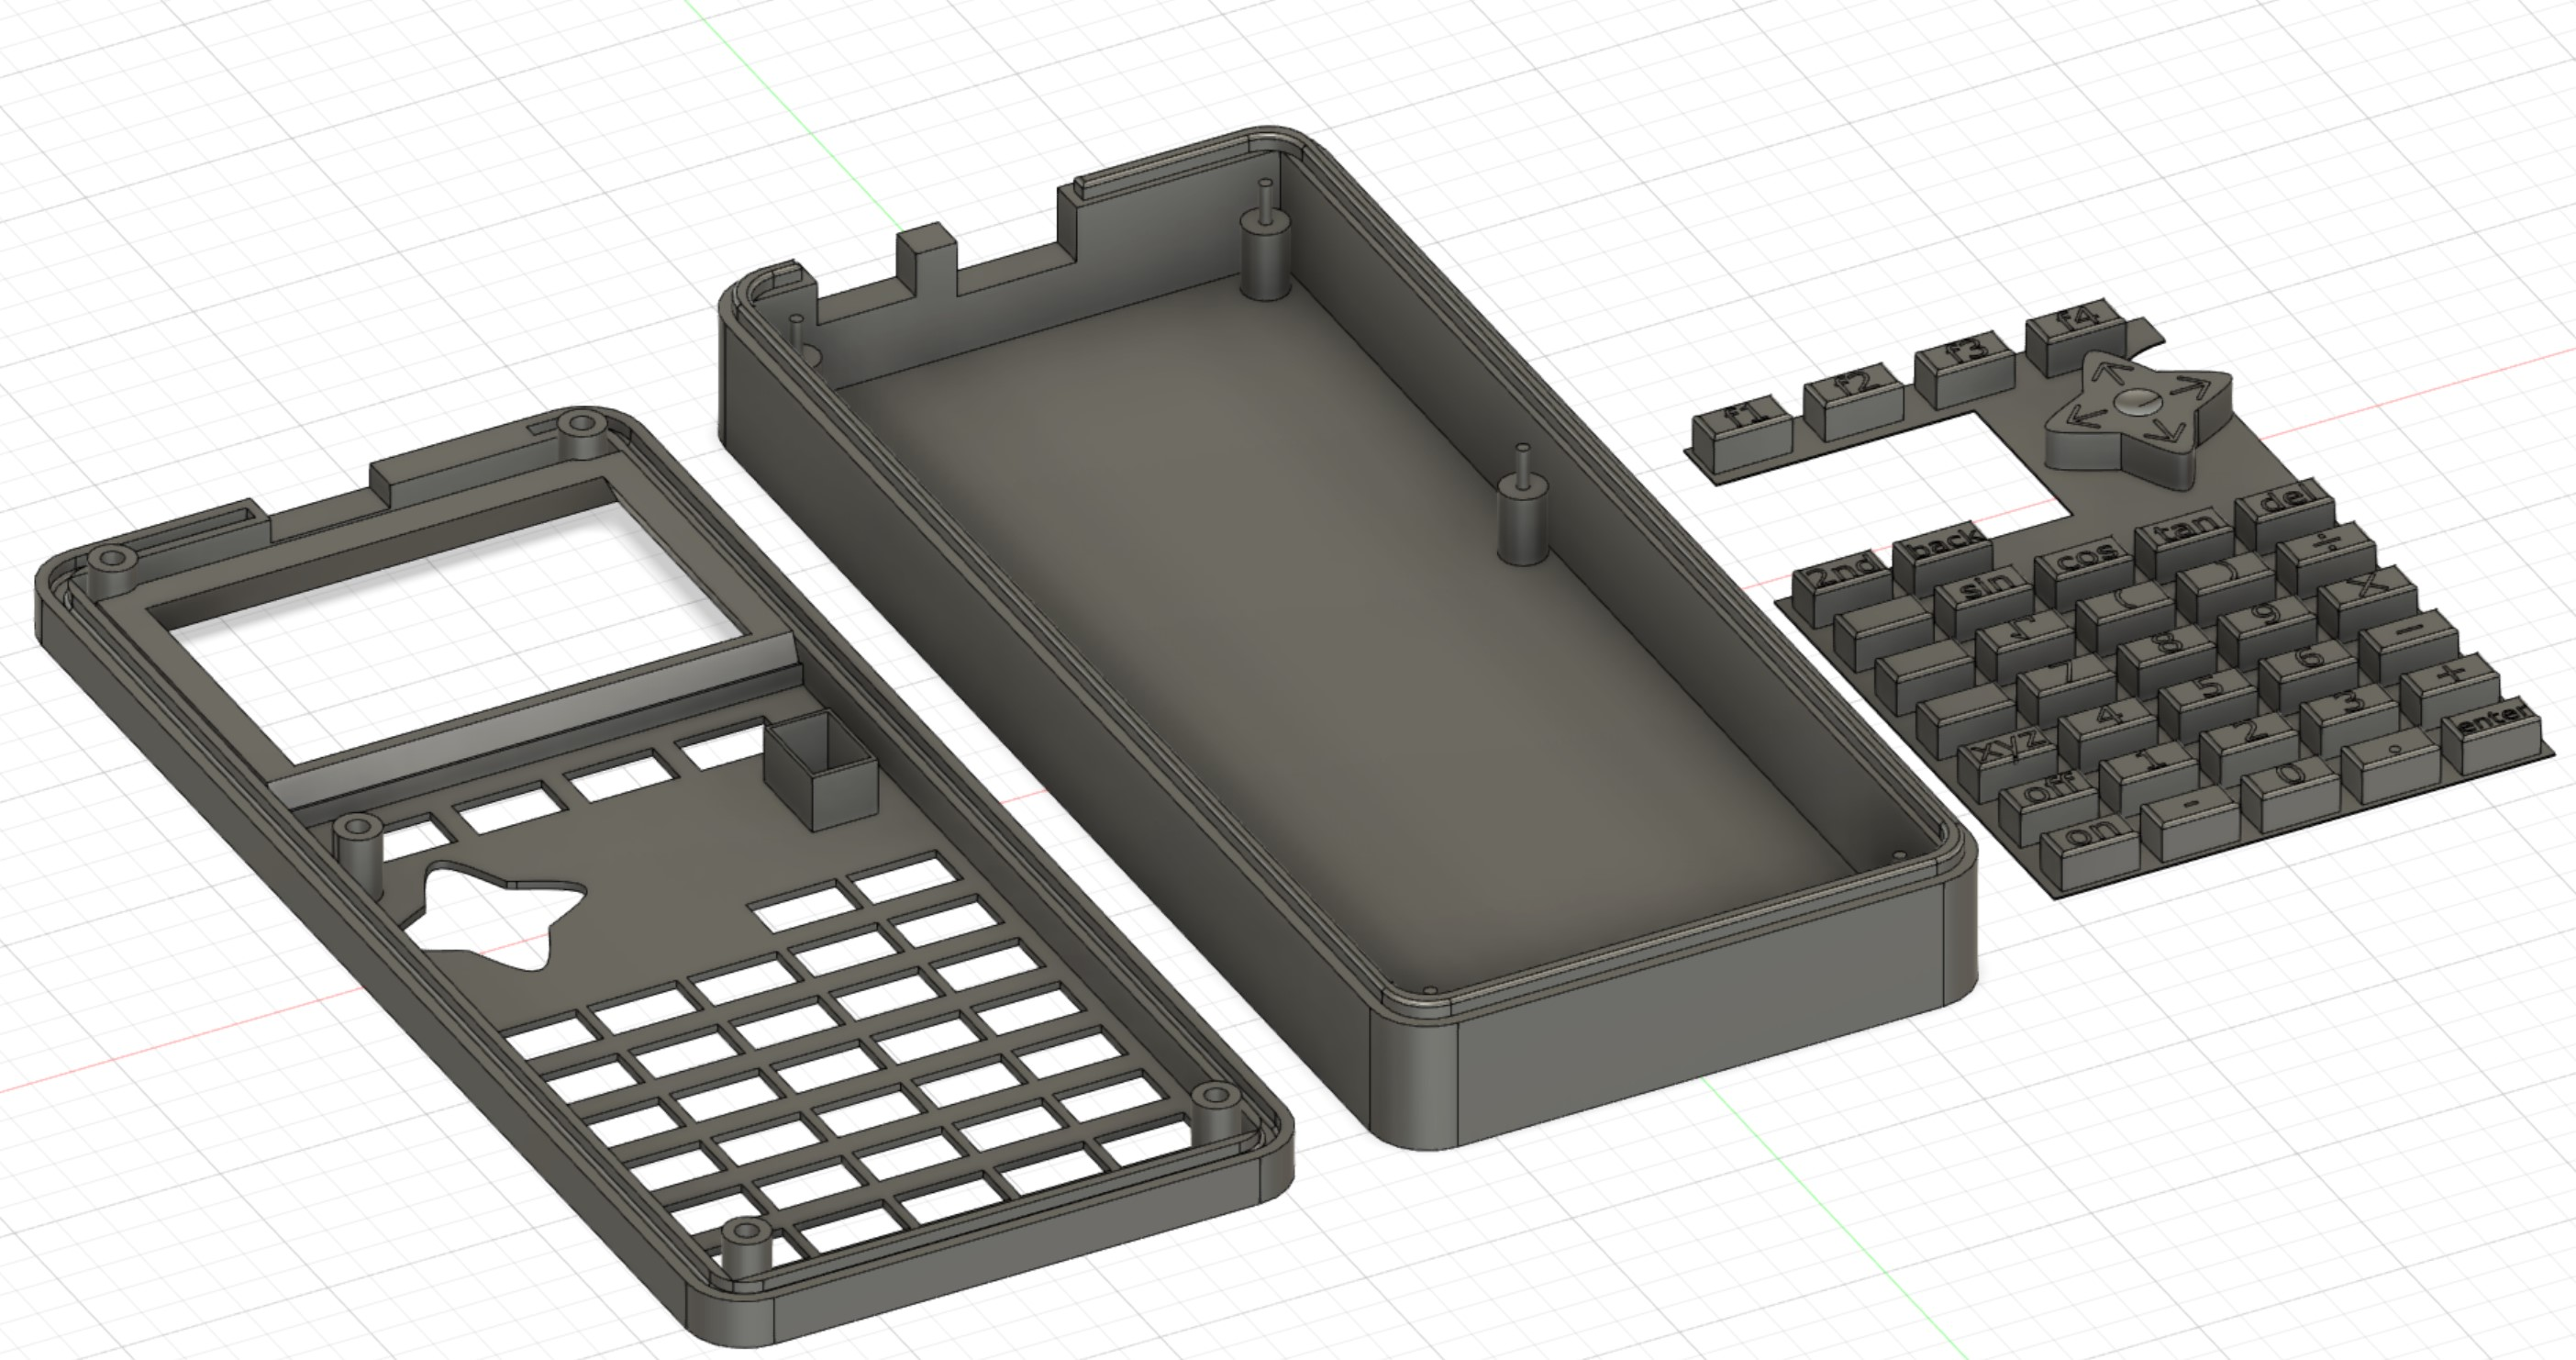
\includegraphics[width=\linewidth]{assets/3dcomponents.jpg}
\end{figure}
In der Basis hat es fünf herausragende Zylinder, die durch die Löcher im PCB gehen sollten und unten für den Akku Platz freimachen. Obwohl ich unzählige Male nachgemessen und berechnet habe, wo diese genau herausragen müssten, waren nie alle am ganz korrekten Ort platziert. Stattdessen wurden beim Zusammenbau vier der fünf kleinen Zylinder entfernt, damit das PCB in das Gehäuse gelegt werden kann, aber weil der Umriss aussen gut gepasst hat, merkt man kaum einen Unterschied. Es war ursprünglich geplant, mit Schrauben das PCB und das Gehäuse festzuhalten, aber aus dieser Idee wurde nichts. Stattdessen hat der Deckel eine Einbuchtung im Rand, die auf das herausragende Stück in der Basis passt und das Knopffeld wird zwischen das PCB und den Deckel gelegt.
\section{Software}
Das Projekt ist auf GitHub unter \url{https://github.com/LetsPlentendo-CH/CALCKS} gehostet, einerseits, damit ich von verschieden Geräten aus weiterarbeiten konnte, anderererseits damit der Quellcode öffentlich sichtbar für Leser dieser Arbeit ist.
Die Projektstruktur ist wie folgt gegliedert (nur Ordner abgebildet):
\dirtree{%
 .1 CALCKS.
 .2 Designs.
 .2 Firmware.
 .3 avr.
 .3 binsend.
 .3 common.
 .3 console.
 .3 eepromgen.
 .3 server.
 .2 Hardware.
 .3 3D Models.
 .3 CALCKS.
}
\subsection{Kompilation}
Im \texttt{Firmware}-Verzeichnis befinden sich eigentlich zwei Versionen der Taschenrechner-Software. Die erste wird für die tatsächliche Hardware, also den ATmega1284, kompiliert. Die zweite wird für die Windows, Mac oder Linux-Konsole kompiliert. Bei dieser Version wird der Bildschirm und die Knöpfe durch Konsolen-Ein- und Ausgabe ersetzt, sodass der simulierte Bildschirm mit einem weiteren Programm angezeigt werden kann. Es wäre aber ziemlich unschön und unübersichtlich, die Codeausschnitte, welche in den zwei Versionen identisch sind, zu duplizieren. Deshalb ist dieser identische Code im Verzeichnis \texttt{common}.
\\[\medskipamount]
Da für den Grossteil des Codes die Hardware mittels selbst geschriebenen Grafik- und Inputlibraries abstrahiert wird, ist es nicht so schwer, die Firmware als Konsolenapplikation zu kompilieren. Dazu müssen nur die Display- und Knopffunktionen neu geschrieben werden, sodass über die Konsole Knopfdrücke eingegeben und der aktuelle Displaystand ausgegeben werden können. Die hardwarespezifischen Dateien sind in \texttt{Firmware/avr} für den Mikroprozessor und \texttt{Firmware/console} für den Emulator.
\subsection{Programmtransfer auf das Gerät}
Von dem ATmega1284 gehen die Pins VCC, GND, MOSI, MISO, SCK und $\overline{\textrm{RESET}}$ zu einem 2x3-Pin-Header. An diesen werden Steckbrückenkabel an einen AVR-Programmer, in meinem Fall an einen Arduino mit einem laufenden ISP-Programm\footnote{Dieses Programm ist in der regulären Arduino-IDE in den Beispielen verfügbar.}, angeschlossen. Das Programm \texttt{avrdude} transferiert das kompilierte Programm über den Arduino zum ATmega1284.
\subsection{Implementation: Text und Grafiken}
Für die Text- und Grafikdarstellung sind die Dateien \texttt{display.c}, \texttt{gui.c} und die dazugehörigen Header-Dateien verantwortlich. \texttt{display.c} sendet die individuellen Befehle an das 128x64 Pixel grosse Display. Das Datasheet des Displaydriver\footnote{Sitronix: Datasheet ST7565R. 2006, S. 50.} (Abbildung \ref{fig:st7565r_ops}) beschreibt die Werte für die vorhandenen Befehle in einer übersichtlichen Tabelle.
\\[\medskipamount]
In der Headerdatei \texttt{display.h} befinden sich für jeden Befehl \textsf{\#define}-Statements, um das Senden dieser Befehle für den Programmierer leserlicher zu machen. Ein kleiner Ausschnitt aus dem Code:
\begin{verbatim}
	...
	#define DISP_CMD_START_LINE 0x40
	#define DISP_CMD_PAGE 0xB0
	#define DISP_CMD_COL_MSB 0x10
	#define DISP_CMD_COL_LSB 0x00
	#define DISP_CMD_ADC 0xA0
	...
\end{verbatim}
\newpage
\begin{figure}[H]
	\centering
	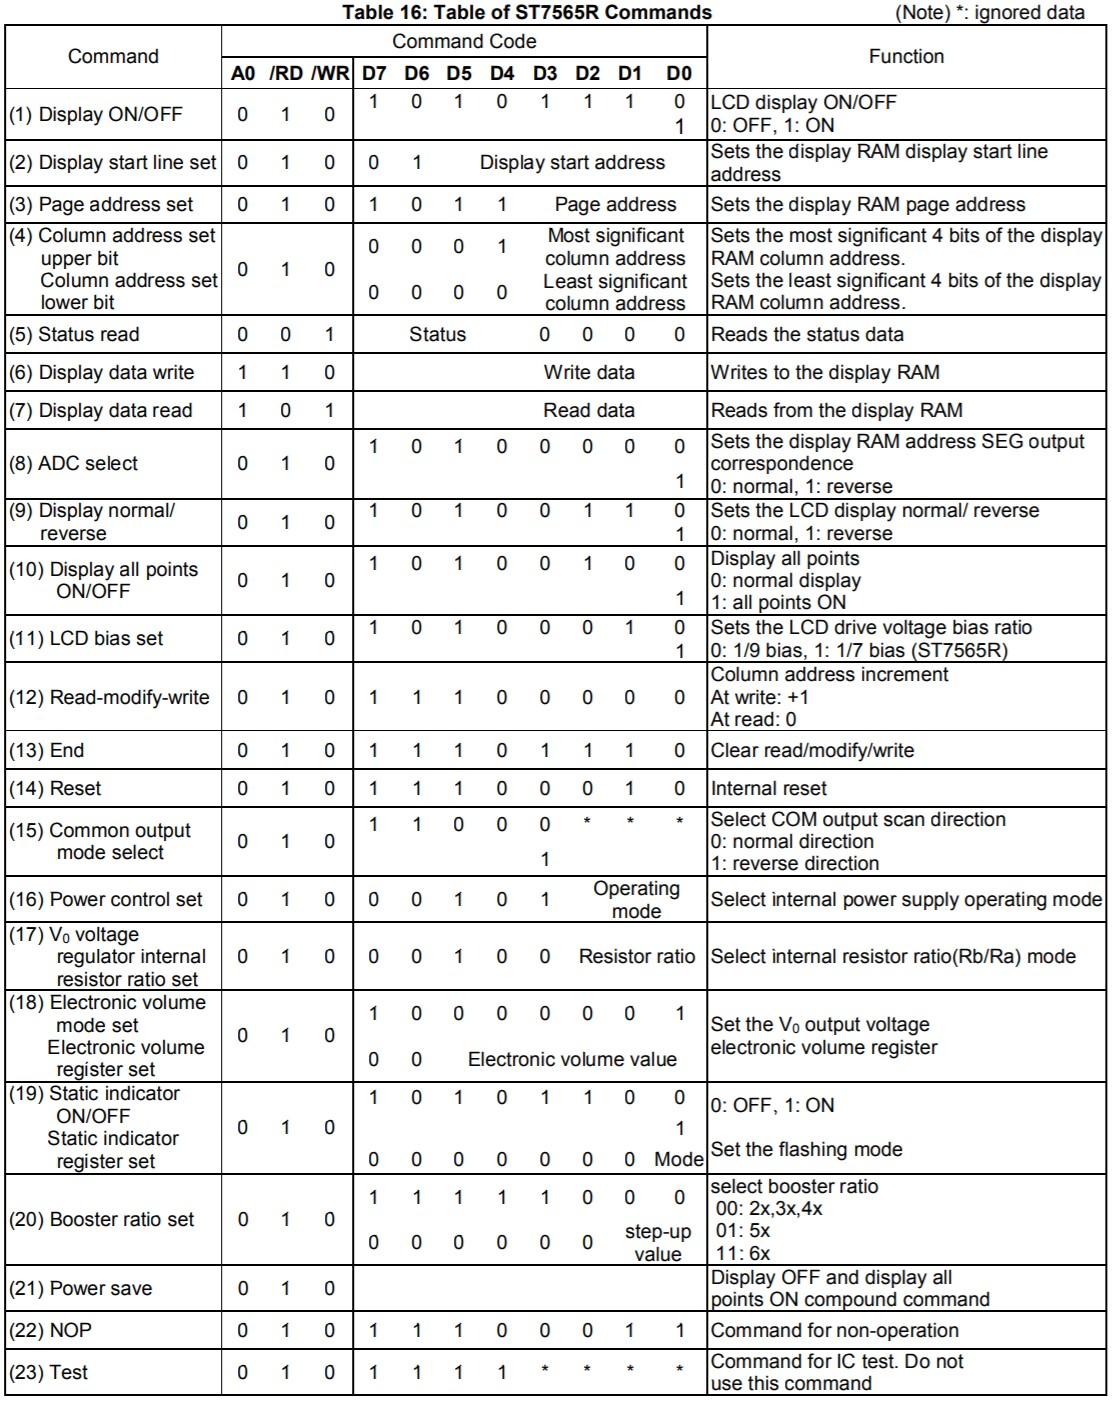
\includegraphics[width=\linewidth]{assets/st7565r_ops.jpg}
	\caption{Die Operationen des Displaytreibers.}
	\label{fig:st7565r_ops}
\end{figure}
Das Datenblatt des LCD-Displays enthält auch eine empfohlene Startsequenz\footnote{Electronic Assembly: Datasheet DOGM128-6. 2009, S. 6.}, die das Display zurücksetzt, den Kontrast setzt und einiges weiteres. Diese kann nun mithilfe diesen \textsf{\#define}-Statements ziemlich leserlich dargestellt werden.
\newpage
\begin{lstlisting}[language=C]
static const char disp_initSequence[DISP_INIT_LEN] = {
    DISP_CMD_START_LINE | 0b000000, // Start at line 0
    DISP_CMD_ADC | 0,               // ADC normal -> left to right
    DISP_CMD_COM_OUT_DIR | 0b1000,  // Select reverse common output
    DISP_CMD_DISP_DIR | 0,          // Set Display direction normal
    DISP_CMD_LCD_BIAS | 0,          // Set bias 1/9 - duty 1/65
    DISP_CMD_POWER_CTRL | 0b111,    // Power control: Booster on, Regulator on, Follower on
    DISP_CMD_BOOSTER_RATIO_MODE,    // Booster ratio:
    0x00,                           // 4x
    DISP_CMD_V0_RATIO | 7,          // V0 Voltage set: 7
    DISP_CMD_ELVOL_MODE,            // Electronic volume mode:
    0x16,                           // 22
    DISP_CMD_INDICATOR_ONOFF | 0,   // Static indicator off
    0x00,                           // Flashing mode: 0
    DISP_CMD_ALL_ONOFF | 0,         // Display all points: no
    DISP_CMD_ONOFF | 1              // Display on
};
\end{lstlisting}
Beim Aufstarten des Taschenrechners wird dieser Array durchiteriert und jeder Befehl an das Display gesendet.
\\[\medskipamount]
Im EEPROM des ATmega1284 sind zwei Schriftarten gespeichert: eine mit Auflösung 6x7 Pixel pro Zeichen und eine mit Auflösung 8x16 Pixel (siehe Abbildung \ref{fig:fontsmall} und \ref{fig:fontmedium}). Die Schiftarten habe ich selbst erstellt in Aseprite, einem Programm, dass für das Zeichnen von Bildern niedriger Auflösung gedacht ist.
\begin{figure}[H]
	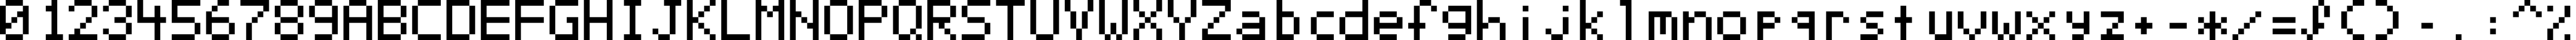
\includegraphics[width=\linewidth]{assets/font6x7l.png}
	\caption{Der 6x7-Font.}
	\label{fig:fontsmall}
\end{figure}
\begin{figure}[H]
	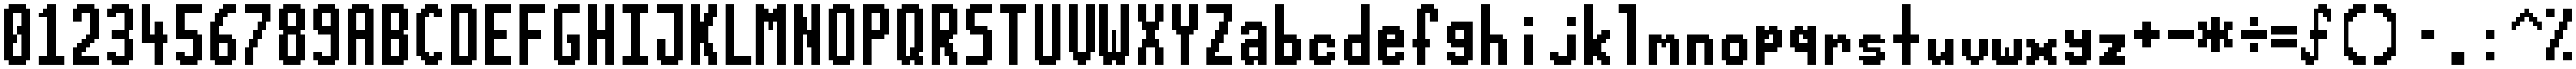
\includegraphics[width=\linewidth]{assets/font8x16l.png}
	\caption{Der 8x16-Font.}
	\label{fig:fontmedium}
\end{figure}
Sowohl diese Schriftarten als auch das Aufstartbild werden mit einem \textit{node.js}-Programm in eine Binärdatei umgewandelt und mit \texttt{avrdude} auf den EEPROM des Mikrocontrollers kopiert.
\\[\medskipamount]
Im Verzeichnis \texttt{Firmware/binsend} befindet sich ein mittlerweise obsoletes Programm, dass von der Zeit des Prototyps auf der Steckplatine stammt. Es wurde auf den Arduino geladen und schrieb die Schriftart und das Aufstartlogo, die der Arduino über USB empfing, in den externen EEPROM.
\subsection{Implementation: Termanalyse}
Das zentralste Element der Software für den Taschenrechner ist das Analysieren von mathematischen Termen. Dies ist nicht nur essentiell für das Ausrechnen von Termen im Hauptbildschirm, sondern auch für das Zeichnen von Graphen. Den Algorithmus, den ich für das Parsen verwendete, ist eine modifizierte Variante des Shunting-yard Algorithmus. Das Grundprinzip ist, dass man von links nach rechts den Term durchläuft und mithilfe eines Stacks die Operandenpriorität erkannt wird. In der Originalvariante des Shunting-yard-Algorithmus entsteht aus einem Term in der Infixnotation, also der, die wir aus dem alltäglichen Leben kennen, in einen Term in der Postfixnotation \footnote{vgl. Hafizji, Ali: Shunting Yard Algorithm}. Diese Postfixnotation hat den Vorteil, dass keine Kenntnisse von Operandenprioritäten wie Punkt vor Strich notwendig sind. Stattdessen steht der Operand immer nach den zwei Operatoren. Zwei Beispiele:
\\[\medskipamount]
\textsf{4 + 3} wäre in der Postfixnotation \textsf{4 3 +} und \textsf{5 * 9 + 2} wäre \textsf{5 9 * 2 +}.
\\[\medskipamount]
Ich habe mich aber entschieden, den Term nicht in eine weitere lineare Struktur umzuformen, sondern in einen Ausdrucksbaum. Dies verkompliziert zwar den Umwandlungsalgorithmus, vereinfacht aber das Ausrechnen eines Terms.
\\
\begin{figure}[H]
	\centering
	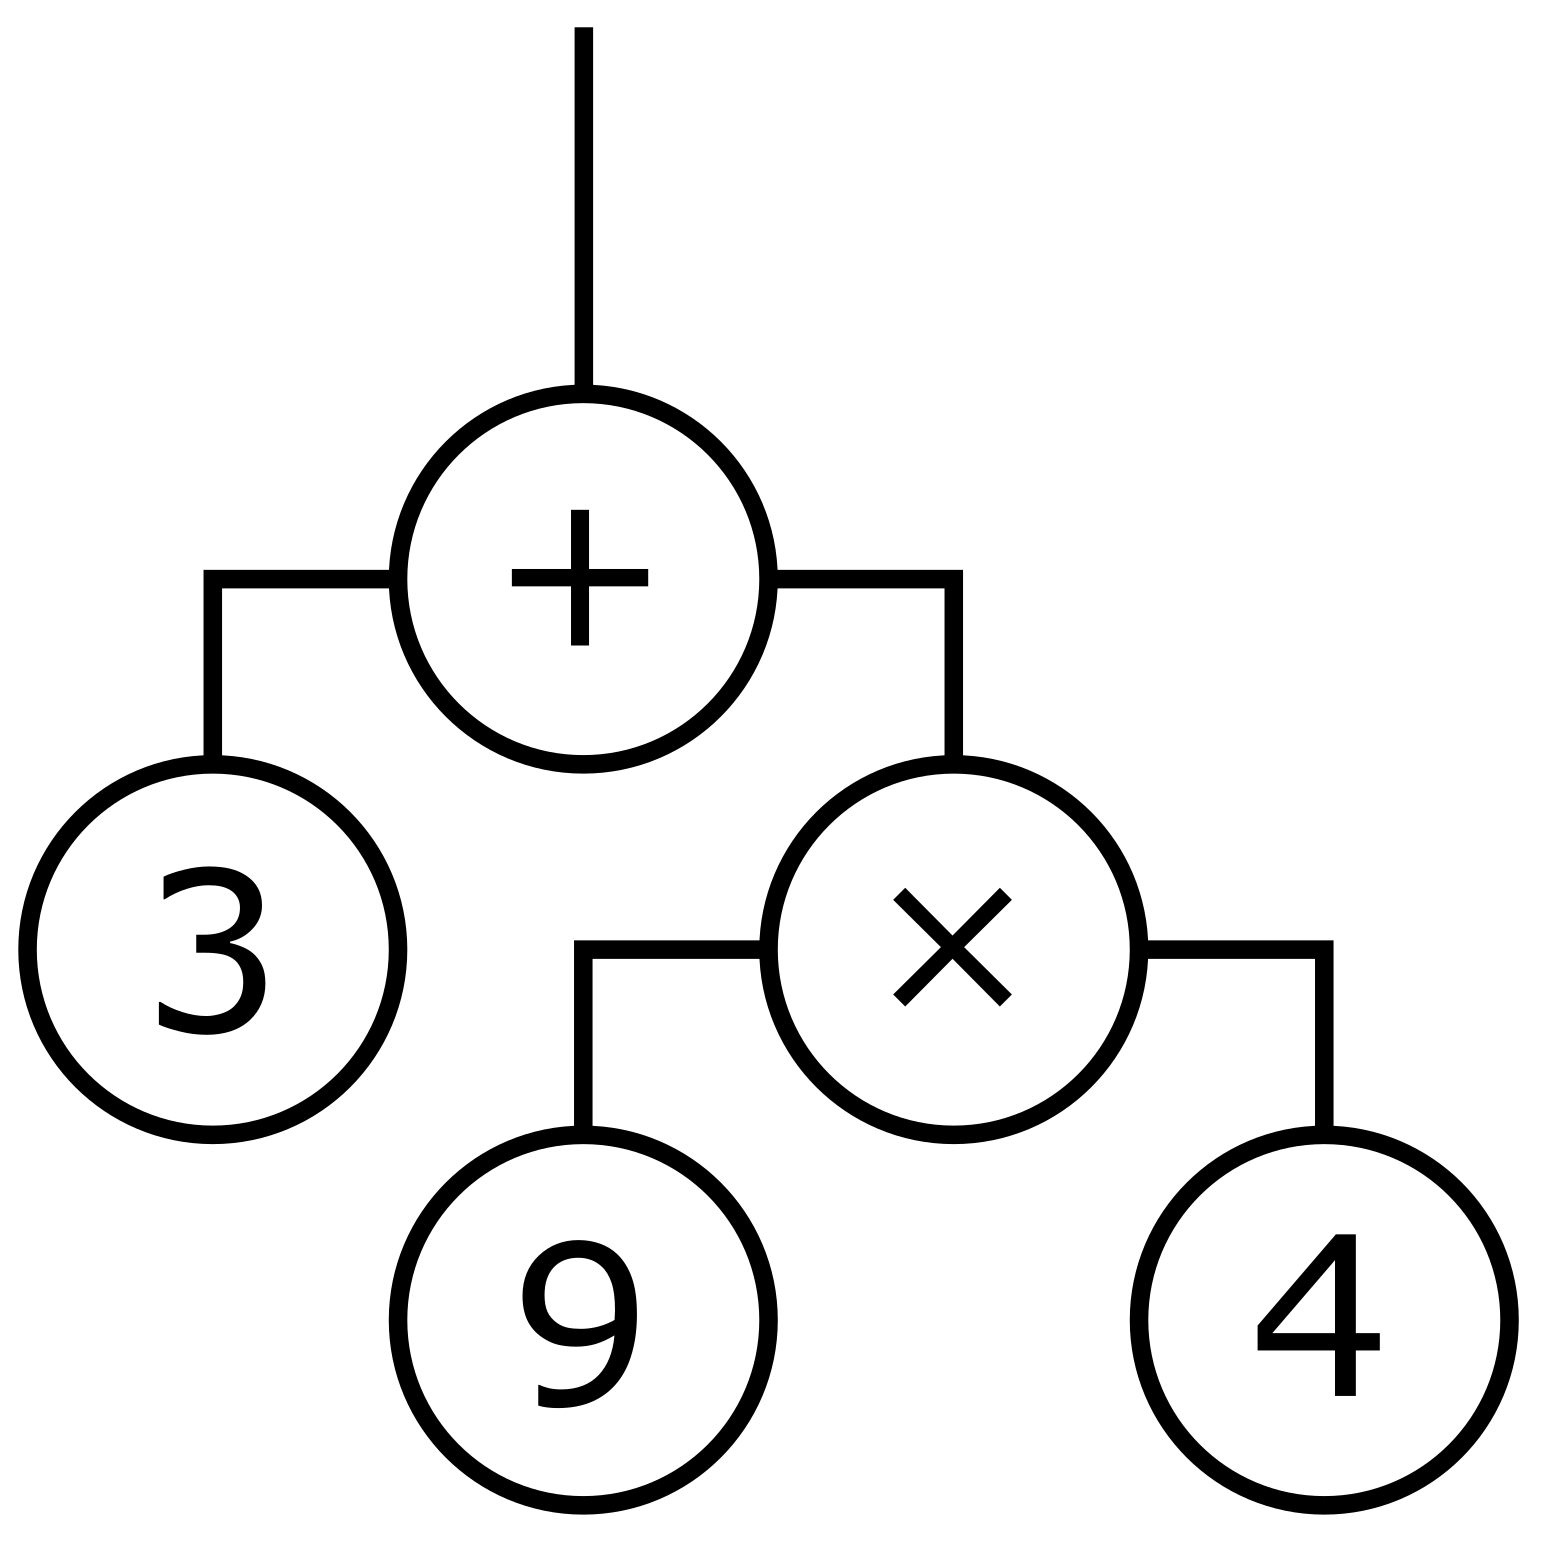
\includegraphics[width=0.2\linewidth]{assets/exprtree1.png}
	\caption{Die häufigste Darstellung eines Ausdrucksbaums.}
	\label{fig:exprtreecommon}
\end{figure}
\begin{figure}[H]
	\centering
	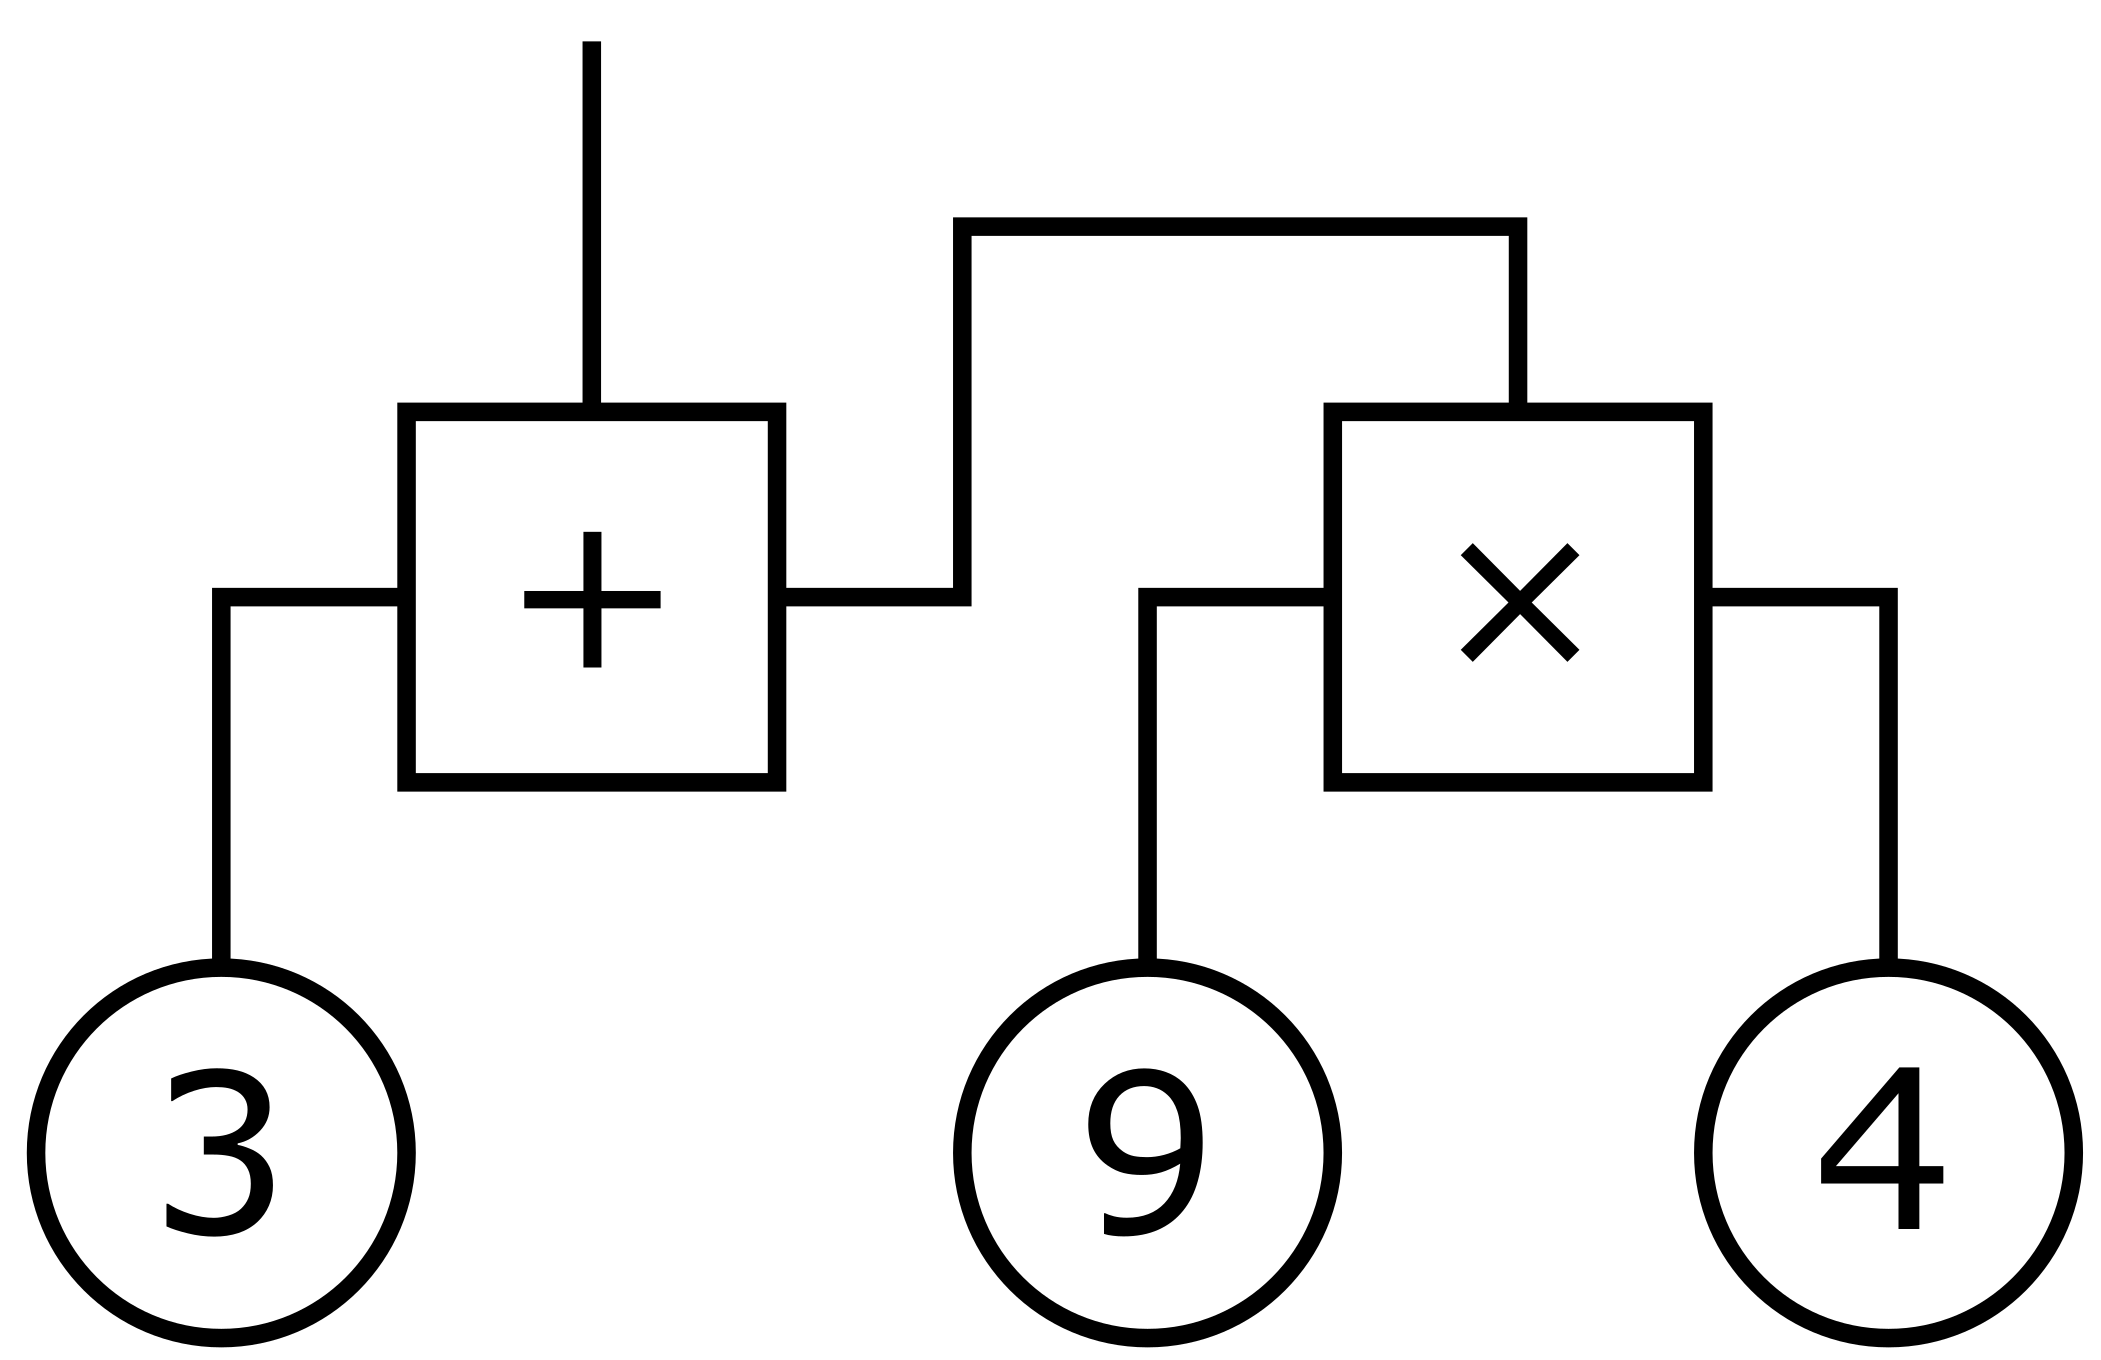
\includegraphics[width=0.2\linewidth]{assets/exprtree2.png}
	\caption{Eine kompaktere Darstellung eines Ausdrucksbaums.}
	\label{fig:exprtreeown}
\end{figure}
Abbildung \ref{fig:exprtreecommon} zeigt die Darstellung eines Ausdrucksbaums, wie man ihn im Mathematikunterricht kennenlernt. Beim Erklären meines Algorithmus macht es aber meiner Meinung nach mehr Sinn, sie etwas kompakter und horizontal darzustellen, wie in Abbildung \ref{fig:exprtreeown}. Bei dieser Darstellung sind die Operanden in Quadraten in der oberen Reihe dargestellt, die Zahlen in Kreisen in der unteren Reihe. 
Die wichtigste Datenstruktur in meiner Implementierung ist der \textsf{opNode}-struct. Dies ist ein Knoten im Ausdrucksbaum, der die dazugehörige mathematische Operation, die beiden Operanden und der Typ der Operanden speichert.
Der Algorithmus folgt nun in Pseudocode.
\newpage
\newgeometry{left=2cm,right=2cm,bottom=2.25cm}
\begin{algorithm}[!ht]
\caption{Umwandlung Infixnotation in Operationsbaum}\label{myalgo}
currValue $\gets$ 0\;
operatorStack $\gets$ []\;
define latestOp\;
\While{\textrm{current character $\neq$ end of input}}{
	curr $\gets$ current character\;
	\uIf{\textrm{type of curr = number}}{
		$\textrm{currValue} \gets \textrm{currValue}*10+\textrm{curr}$\;
	}
	\uElseIf{\textrm{type of curr = operator}}{
		$\textrm{latestOp} \gets \textrm{create opNode}(\textrm{curr})$\;
		latestOp.leftOperand $\gets$ currValue\;
		latestOp.operation $\gets$ operation of curr\;
		\If{\textrm{operatorStack.size} $\neq$ \textrm{0}}{
			\If{$\textrm{precedence(latestOp.operation)} \leq \textrm{precedence(operatorStack.top.operation)}$}{
				$\textrm{currStackOp} \gets \textrm{operatorStack.top}$\;
				\While{$\textrm{currStackOp} \neq \textrm{undefined and precedence(latestOp.operation)} \leq \textrm{precedence(currStackOp.operation)}$}{
					$\textrm{currStackOp} \gets \textrm{currStackOp.prev}$\;
				}
				$\textrm{latestOp.leftOperand} \gets \textrm{currStackOp}$\;
				\While{$\textrm{currStackOp.next} \neq \textrm{undefined}$}{
					$\textrm{nextOpInStack} \gets \textrm{currStackOp.next}$\;
					$\textrm{currStackOp.rightOperand} \gets \textrm{nextOpInStack}$\;
					$\textrm{remove currStackOp from operatorStack}$\;
					$\textrm{currStackOp} \gets \textrm{nextOpInStack}$\;
				}
				$\textrm{currStackOp.rightOperand} \gets \textrm{currValue}$\;
				$\textrm{remove currStackOp from stack}$\;
			}
		}
		operatorStack.push(latestOp)\;
		currValue $\gets$ 0\;
	}
	Move to next character in input\;
}
$\textrm{latestOp.rightOperand} \gets \textrm{currValue}$\;
remove latestOp from operatorStack\;
\While{\textrm{operatorStack.size $\neq$ 0}}{
	operatorStack.top.rightOperand $\gets$ latestOp\;
	$\textrm{latestOp} \gets \textrm{operatorStack.top}$\;
	remove operatorStack.top from operatorStack\;
}
\tcc{Die oberste Operation im Ausdrucksbaum is nun latestOp.}
\end{algorithm}
\restoregeometry
In der Form von Programmcode gibt es noch einige Spezialfälle, die eingebaut werden mussten. Zum Beispiel: Wenn eine Eingabe nur aus einer einzigen Zahl oder Variable besteht, hat der Algorithmus keinen Operator-Knoten, wo diese einzelne Zahl oder Variable eingesetzt werden könnte. Stattdessen erstellt das Programm in diesem Fall einen Plus-Operator-Knoten mit 0 als erster Operand und der Zahl oder Variable als zweiter Operand.
Im Pseudocode sind ausserdem keine Klammern erwähnt, weil diese den Pseudocode sehr unleserlich gemacht hätten. Interessierte Leser können die volle Implementation in der Datei \texttt{Firmware/common/term.c} finden.
\\[\medskipamount]
Es folgt eine Anwendung dieses Algorithmus am Beispielsterm $3+44*2-1$. Der erste Schritt stellt den Ausgangszustand dar. Jeder folgende Schritt ist der Zustand nach jedem Durchlauf der While-Schlaufe, die über alle Zeichen iteriert. Der letzte Schritt ist der Zustand am Ende des Algorithmus.
\begin{center}
\begin{tabular}{ |l|l|c|c| } 
	\hline
	\textbf{Schritt} & \textbf{currValue} & \textbf{Operatoren} & \textbf{operatorStack} \\ 
	\hline
	1 & 0 & (leer) & (leer) \\
	\hline
	2 & 3 & (leer) & (leer) \\ 
	\hline
	3 & 0 & 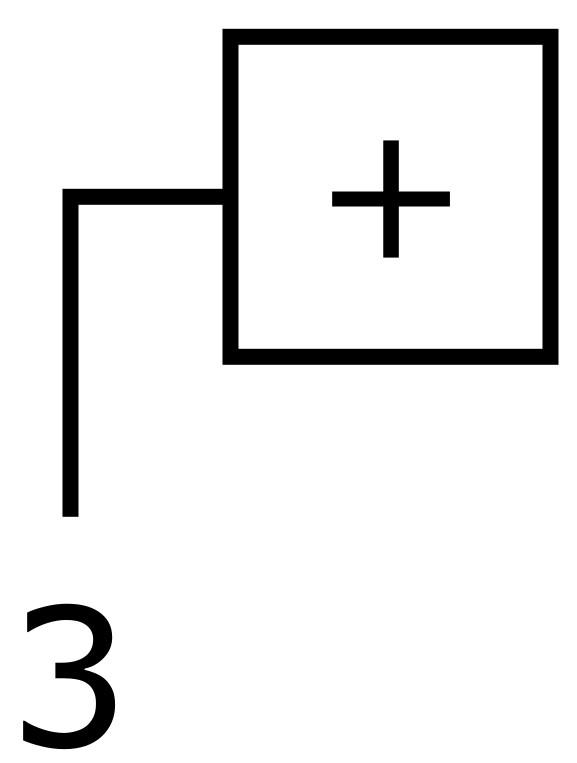
\includegraphics[trim=0 -2 0 -2,height=0.06\textheight]{assets/expr0.jpg} & $+$ \\ 
	\hline
	4 & 4 & 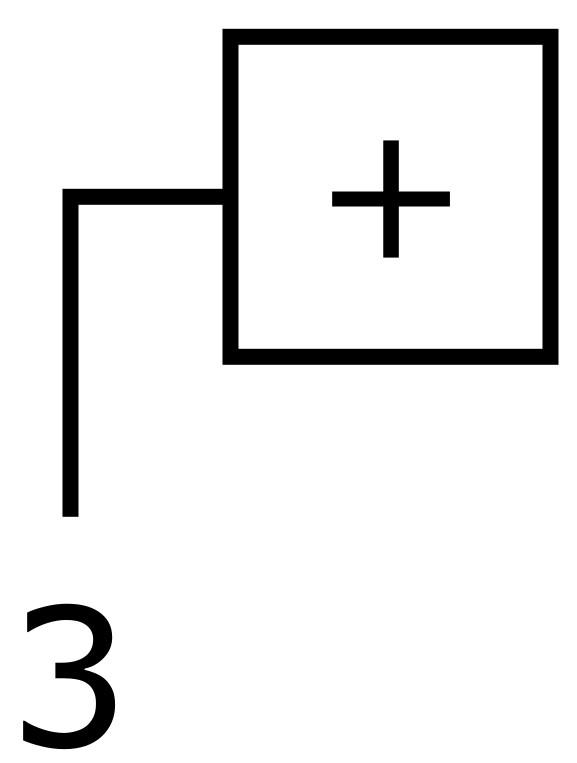
\includegraphics[trim=0 -2 0 -2,height=0.06\textheight]{assets/expr0.jpg} & $+$ \\ 
	\hline
	5 & 44 & 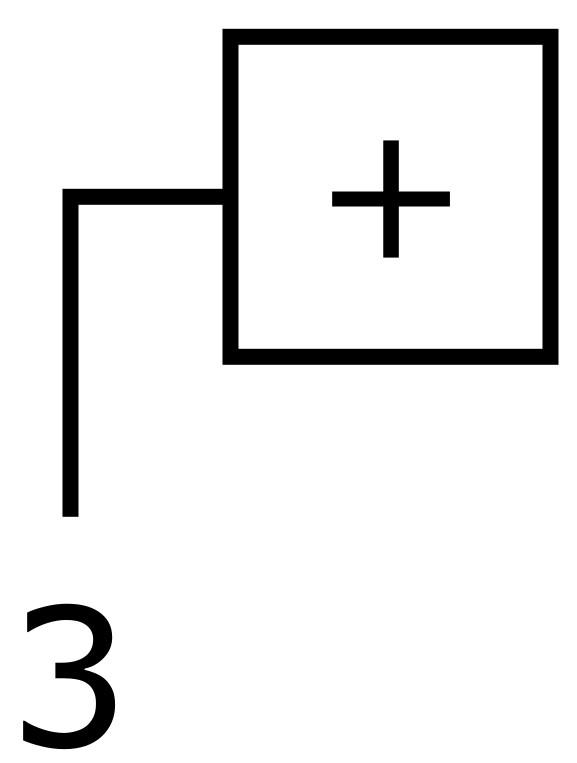
\includegraphics[trim=0 -2 0 -2,height=0.06\textheight]{assets/expr0.jpg} & $+$ \\ 
	\hline
	6 & 0 & 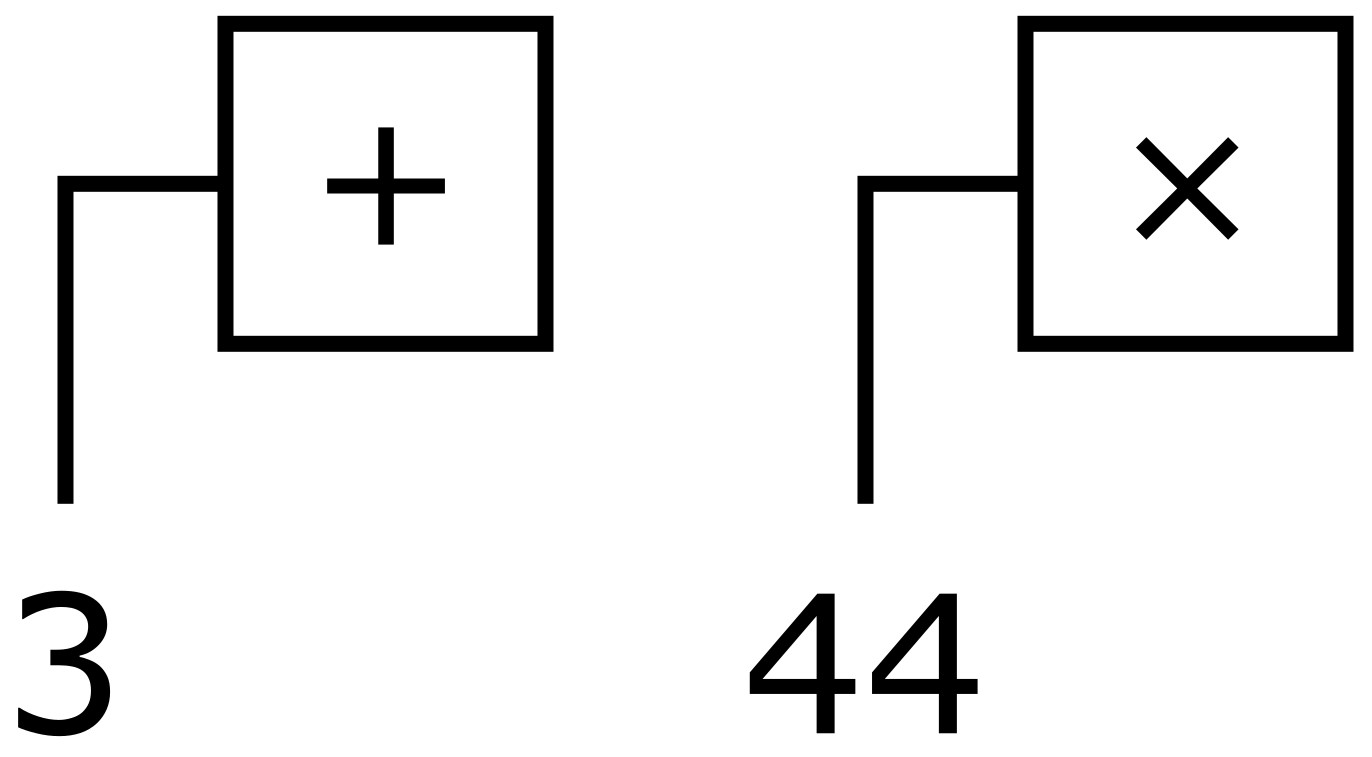
\includegraphics[trim=0 -2 0 -2,height=0.06\textheight]{assets/expr1.jpg} & $+, *$ \\ 
	\hline
	7 & 2 & 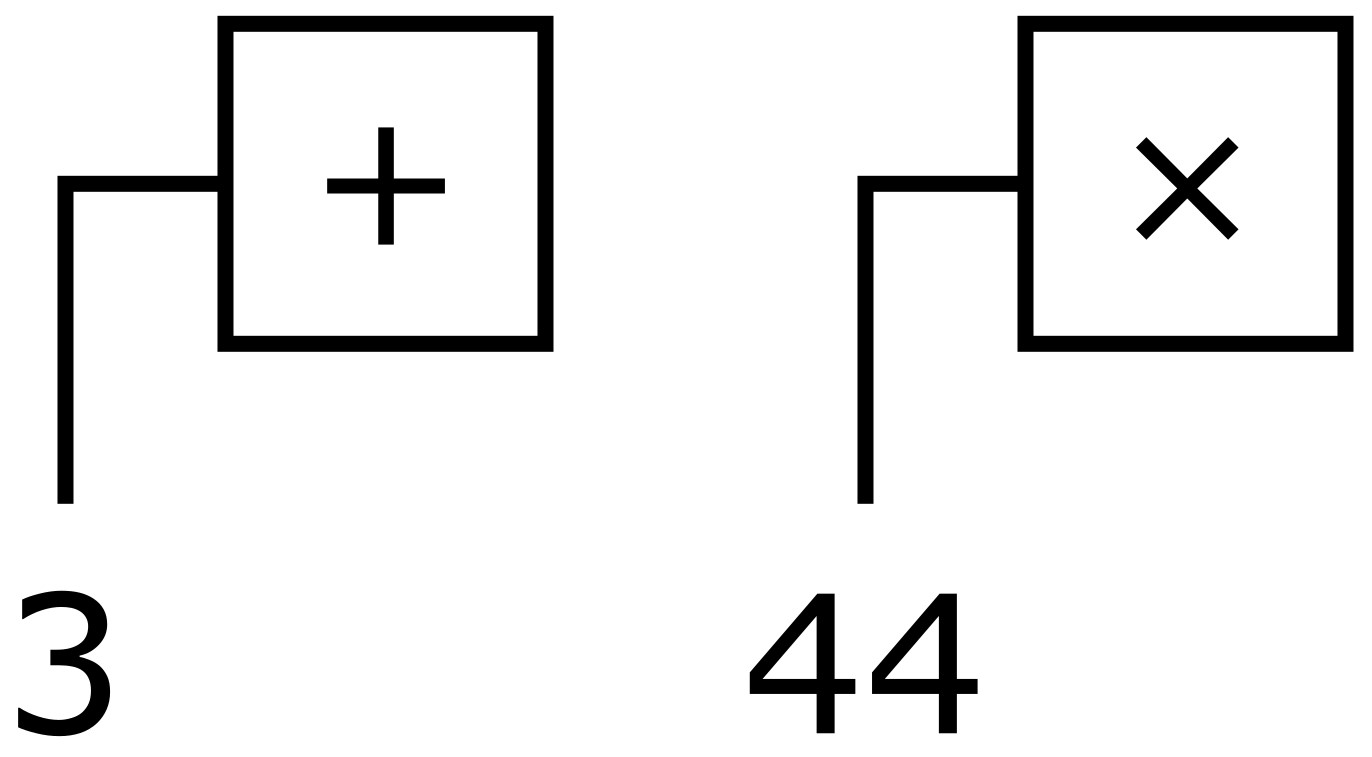
\includegraphics[trim=0 -3 0 -3,height=0.06\textheight]{assets/expr1.jpg} & $+, *$ \\ 
	\hline
	8 & 0 & 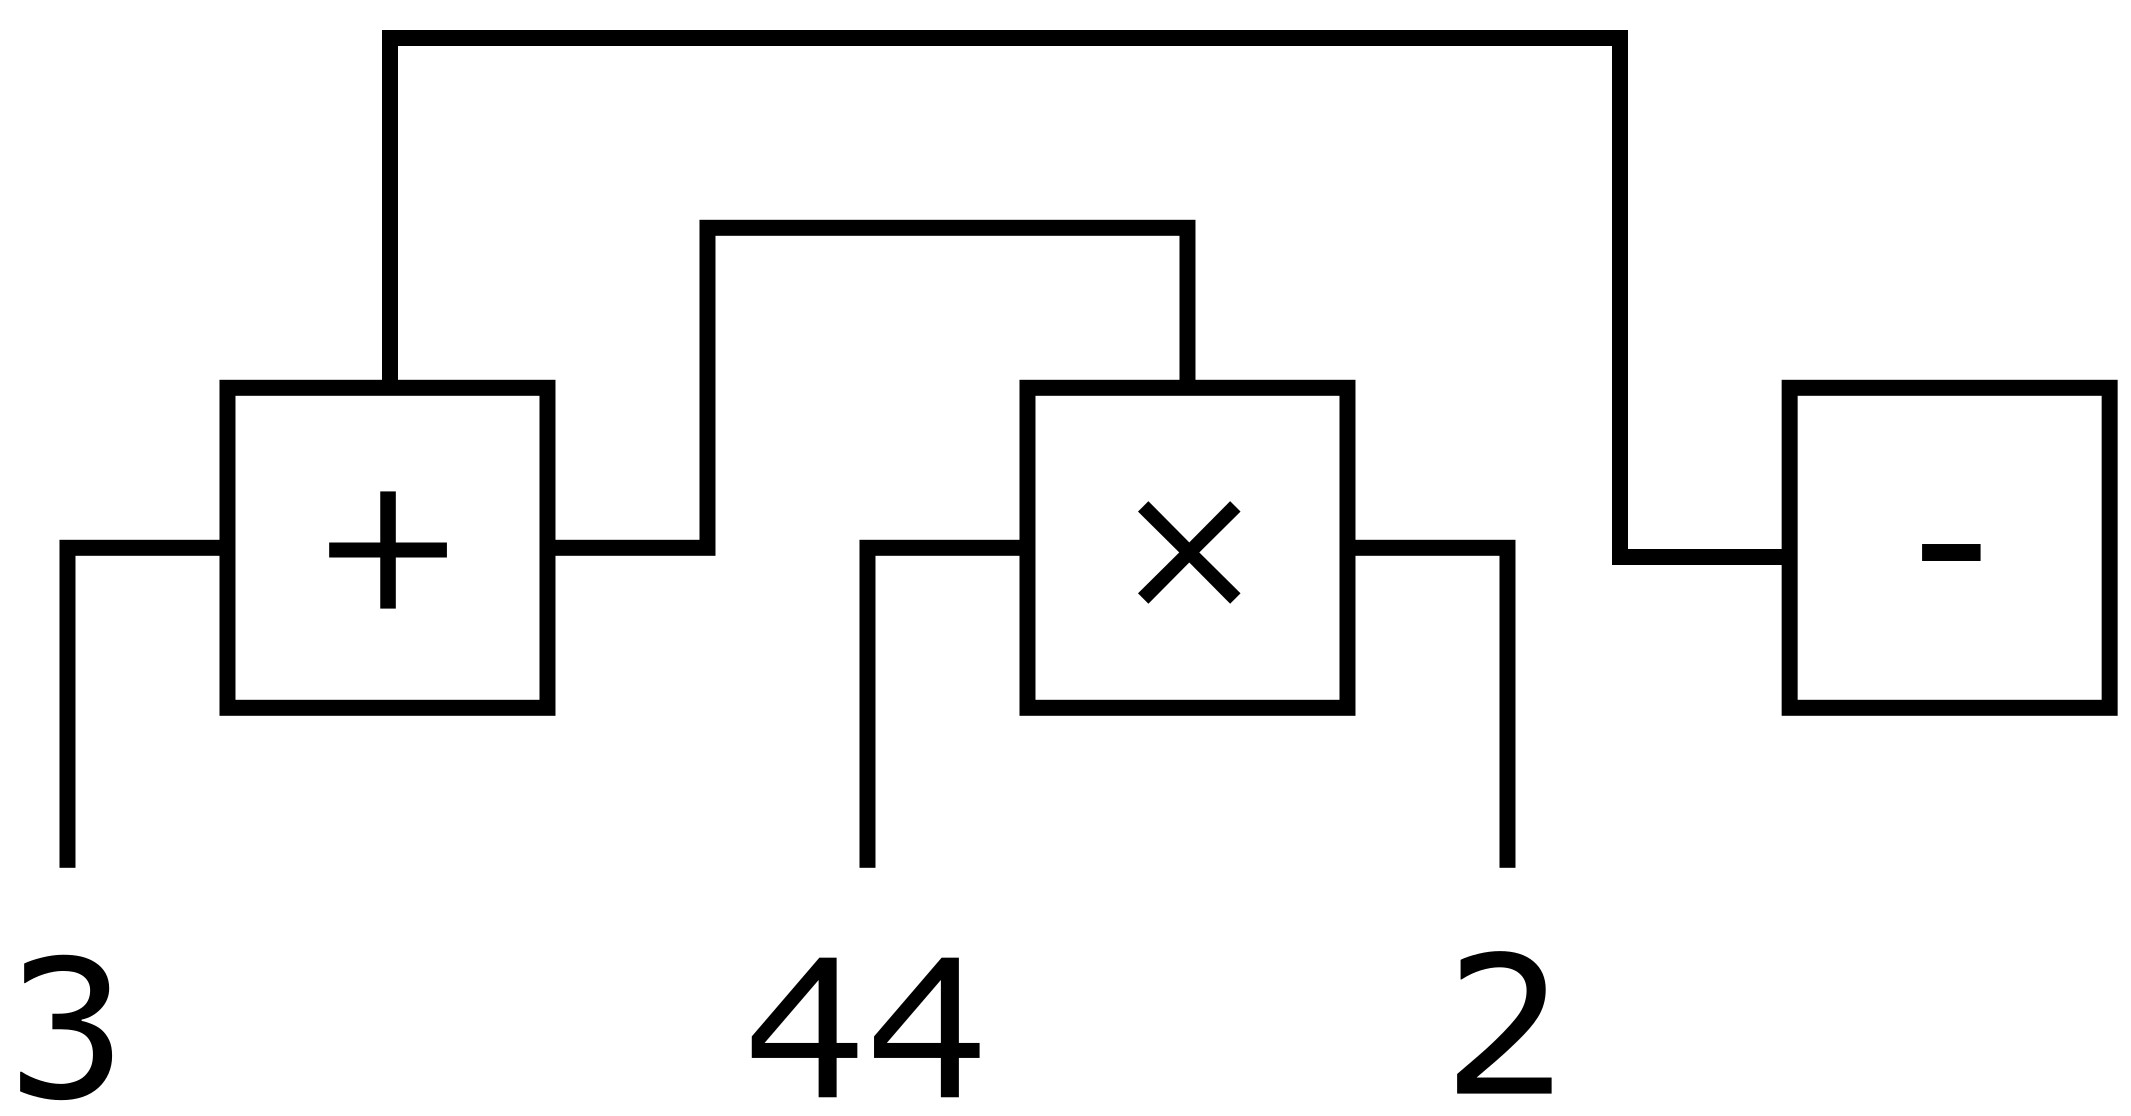
\includegraphics[trim=0 -3 0 -3,height=0.09\textheight]{assets/expr2.jpg} & $-$ \\
	\hline
	9 & 1 & 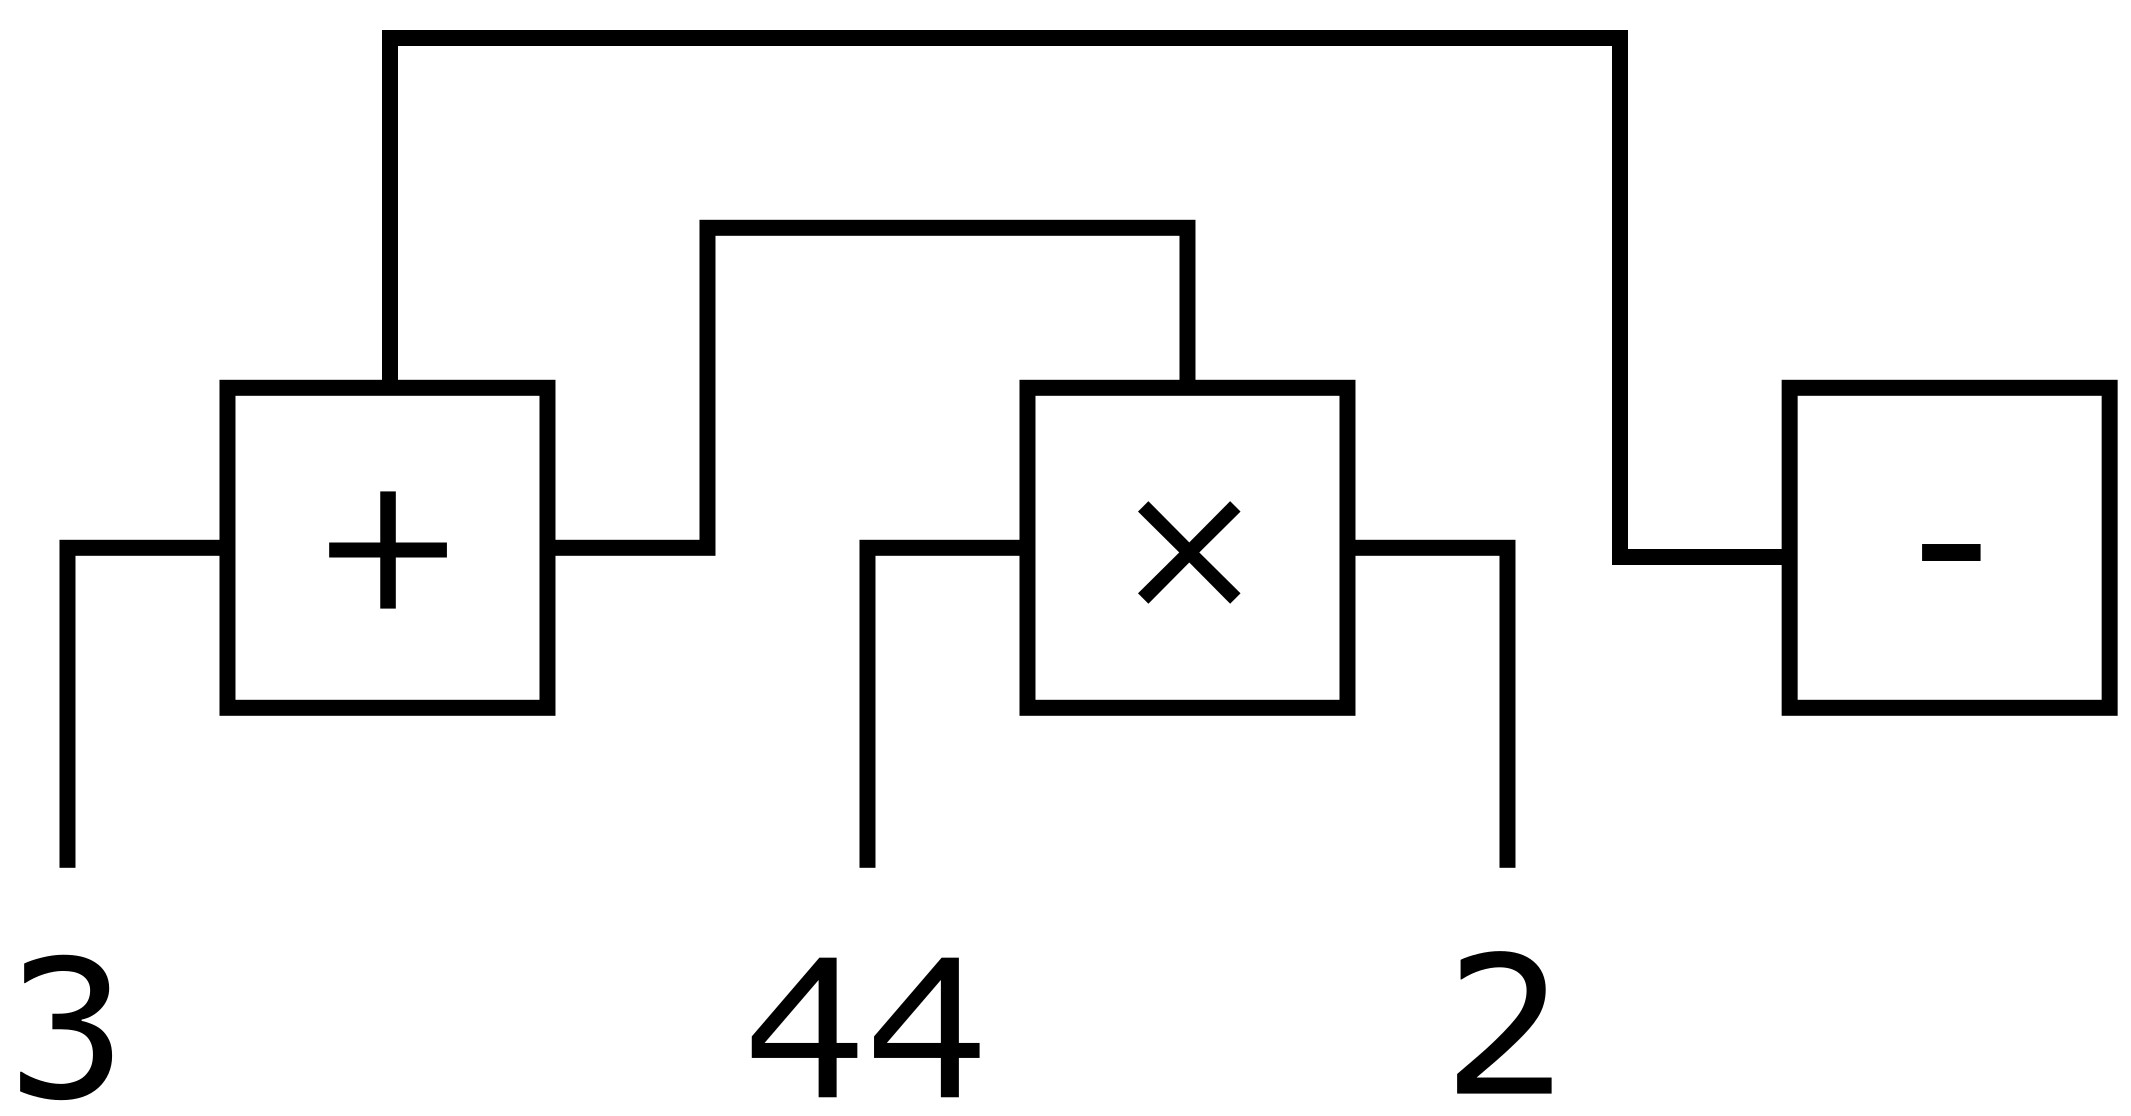
\includegraphics[trim=0 -2 0 -3,height=0.09\textheight]{assets/expr2.jpg} & $-$ \\ 
	\hline
	10 & 0 & 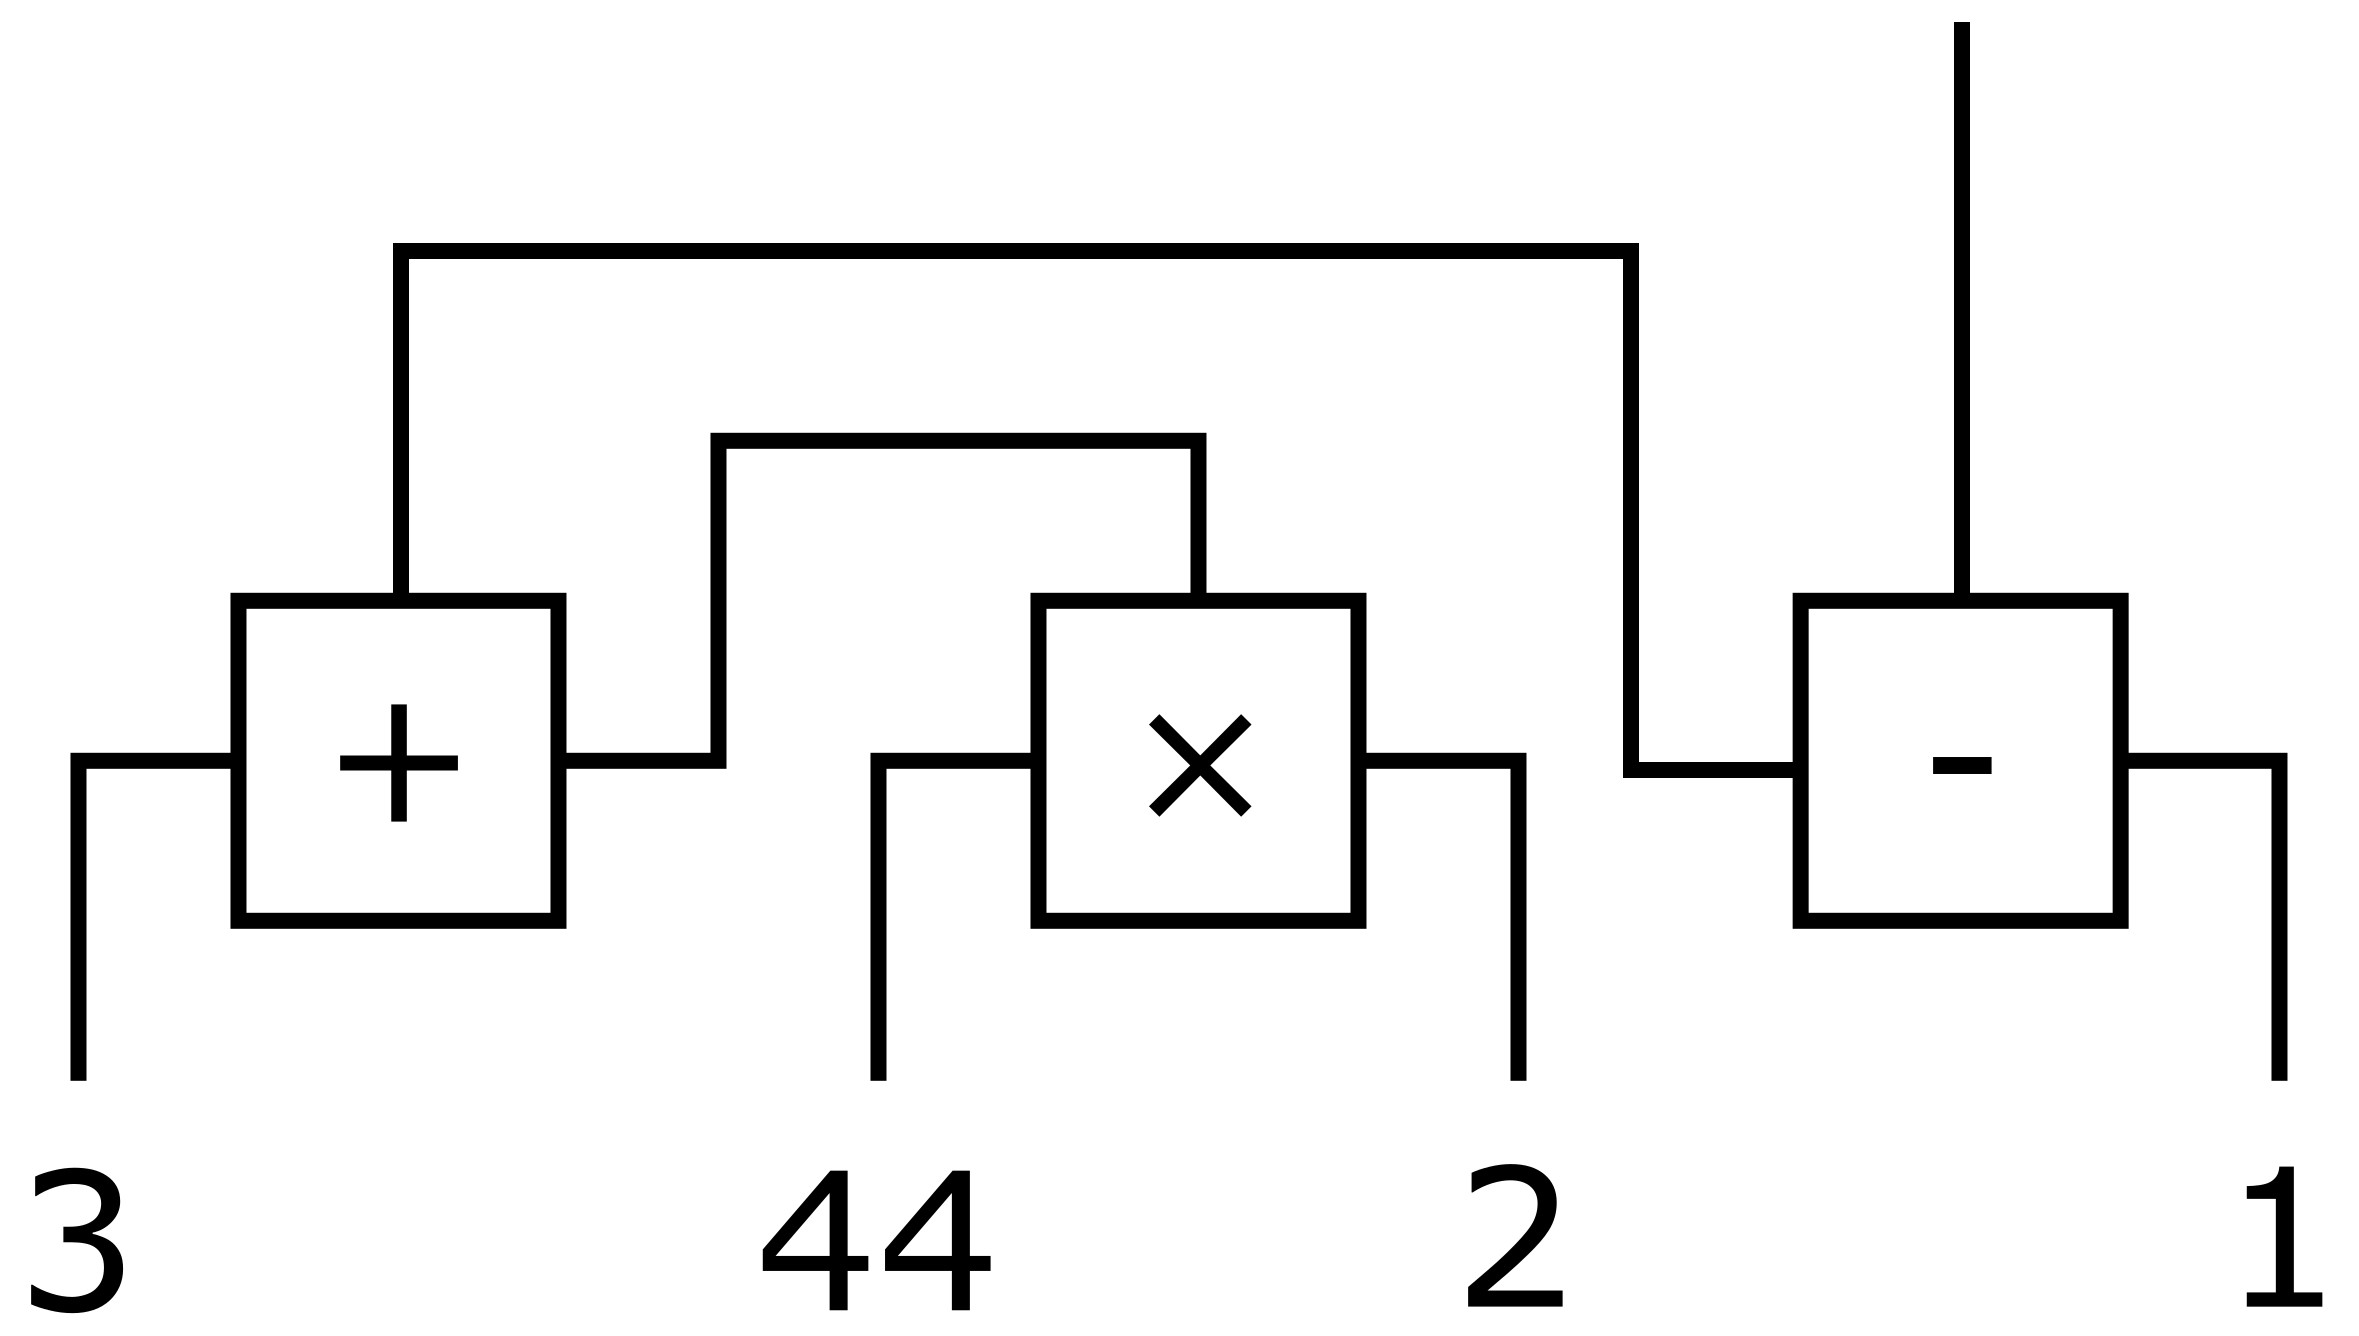
\includegraphics[trim=0 -2 0 -3,height=0.11\textheight]{assets/expr3.jpg} & (leer) \\ 
	\hline
\end{tabular}
\end{center}
\chapter{Resultate}
\section{Aussehen}
\begin{figure}[H]
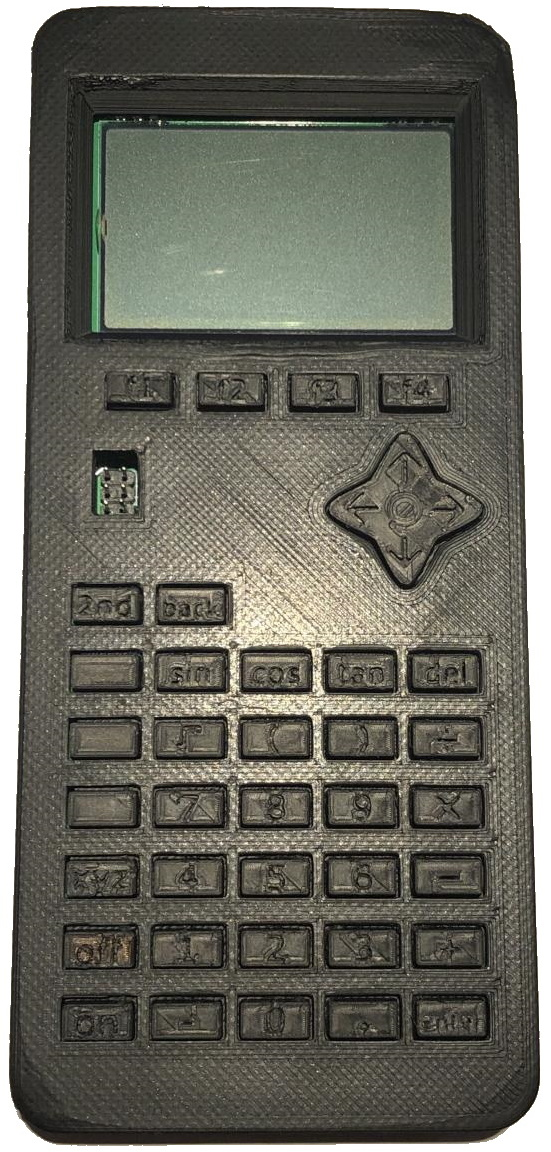
\includegraphics[height=10.5cm]{assets/calcincase.JPG}
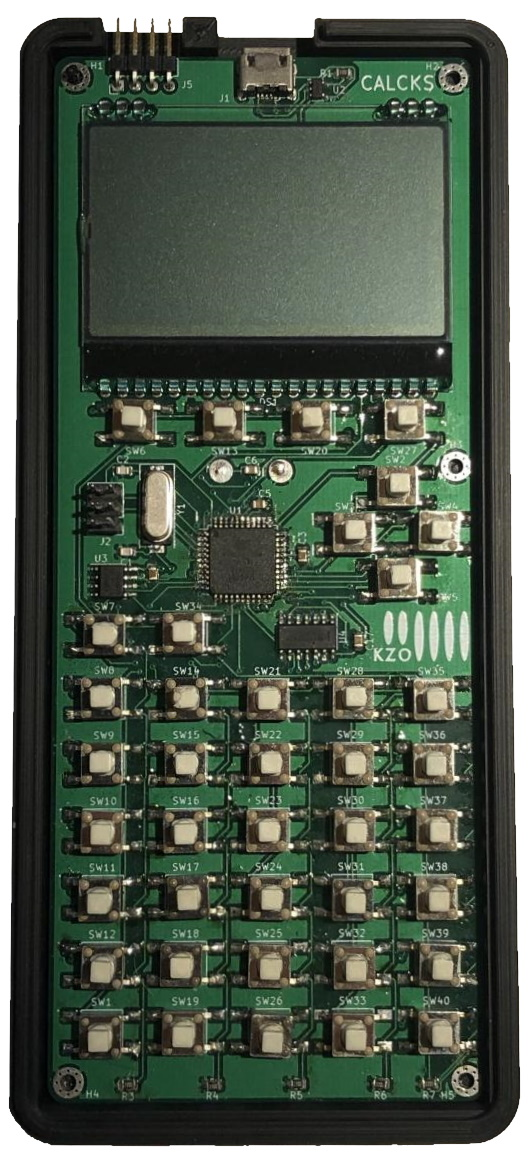
\includegraphics[height=10.5cm]{assets/calctoppcb.JPG}
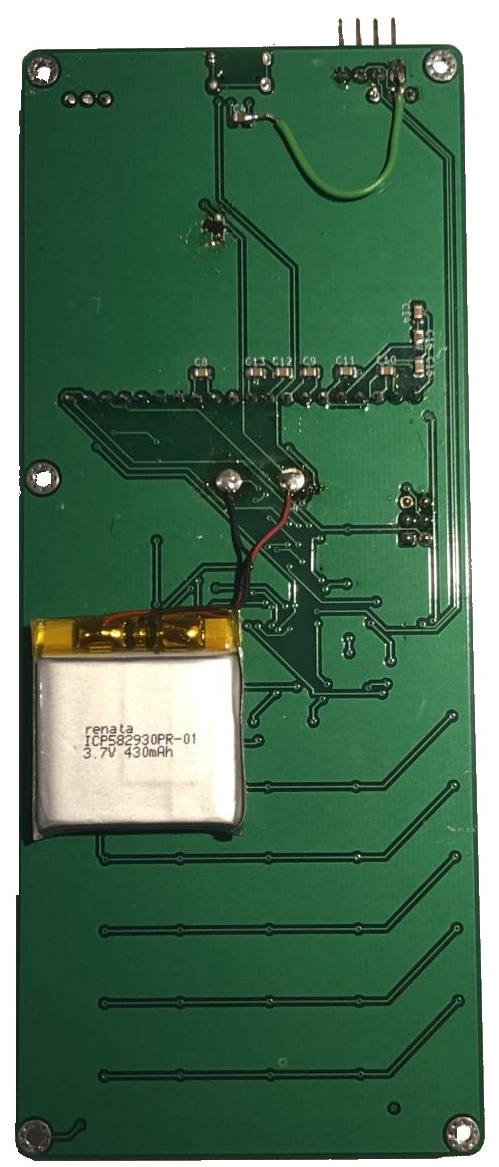
\includegraphics[height=10.6cm]{assets/calcbottompcb.JPG}
\caption{Drei Ansichten des Taschenrechners.}
\label{fig:calcview}
\end{figure}

Abbildung \ref{fig:calcview} zeigt den Taschenrechner in dem Gehäuse und die Ober- und Unterseite des PCBs. In der dritten Abbildung sieht man oben rechts das in Kapitel \ref{secondproto} erwähnte Kabel, das angelötet wurde, damit der Taschenrechner aufladbar ist.

\newpage

\section{Funktionalität}
Beim Aufstarten des Taschenrechners wird man von diesem Logo gegrüsst.

\begin{figure}[H]
\centering
\fbox{
\includegraphics[width=0.4\linewidth]{assets/startup_lg.png}}
\caption{Das Aufstart-Logo des Taschenrechners.}
\end{figure}

\noindent
Danach sieht man den Hauptbildschirm, wo Rechnungen eingegeben werden können. Die vier Tabs unten geben Auskunft, welches Menu die vier Funktionstasten f1 bis f4 öffnen.

\begin{figure}[H]
\centering
\fbox{
\includegraphics[width=0.4\linewidth]{assets/mainscreen_calc_l.png}}
\caption{Der Hauptbildschirm des Taschenrechners.}
\end{figure}

\noindent
Mit den Zahlen- und Operationstasten kann man eine Rechnung eingeben und mit der Enter-Taste berechnen lassen. Zum Zeitpunkt der Abgabe der Arbeit unterstützt der Taschenrechner die folgenden Operationen:
\\
\begin{itemize}
\item Grundoperationen Plus, Minus, Mal, Durch
\item Klammern
\item Potenzen
\end{itemize}

\begin{figure}[H]
\centering
\fbox{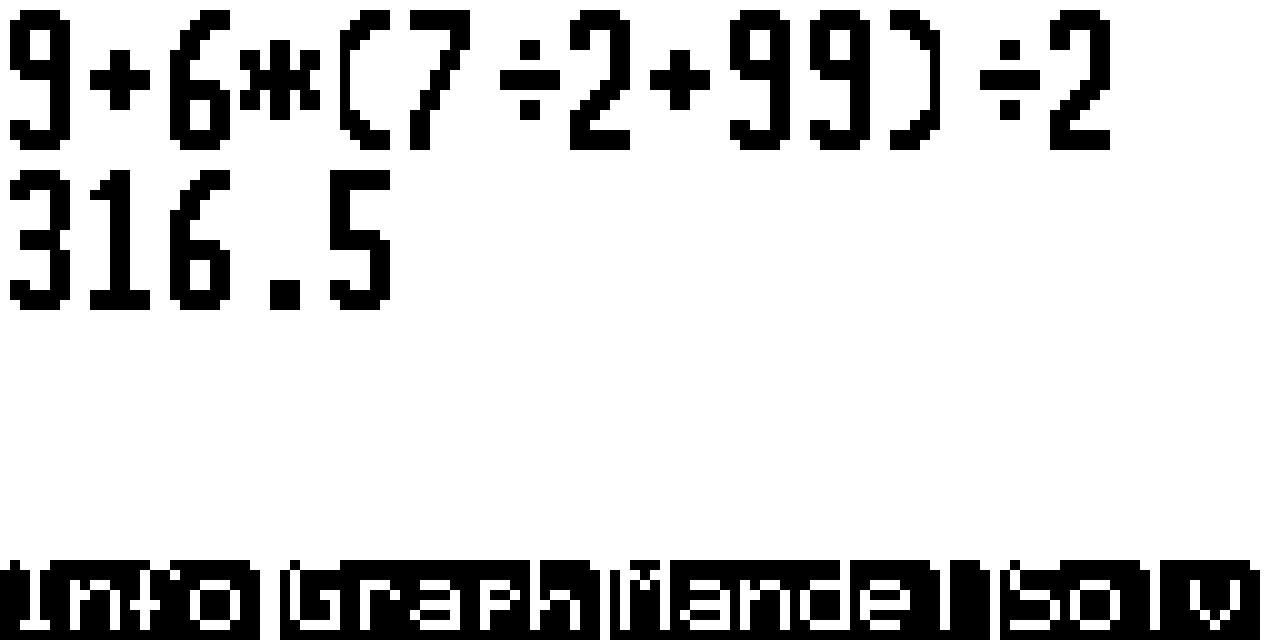
\includegraphics[width=0.4\linewidth]{assets/calc_example_l.png}}
\caption{Eine Beispielsrechnung.}
\end{figure}

\noindent
Drückt man die f1-Taste, führt dies zum Info-Bildschirm, der Versionsnummer und Akkustand anzeigt.

\begin{figure}[H]
\centering
\fbox{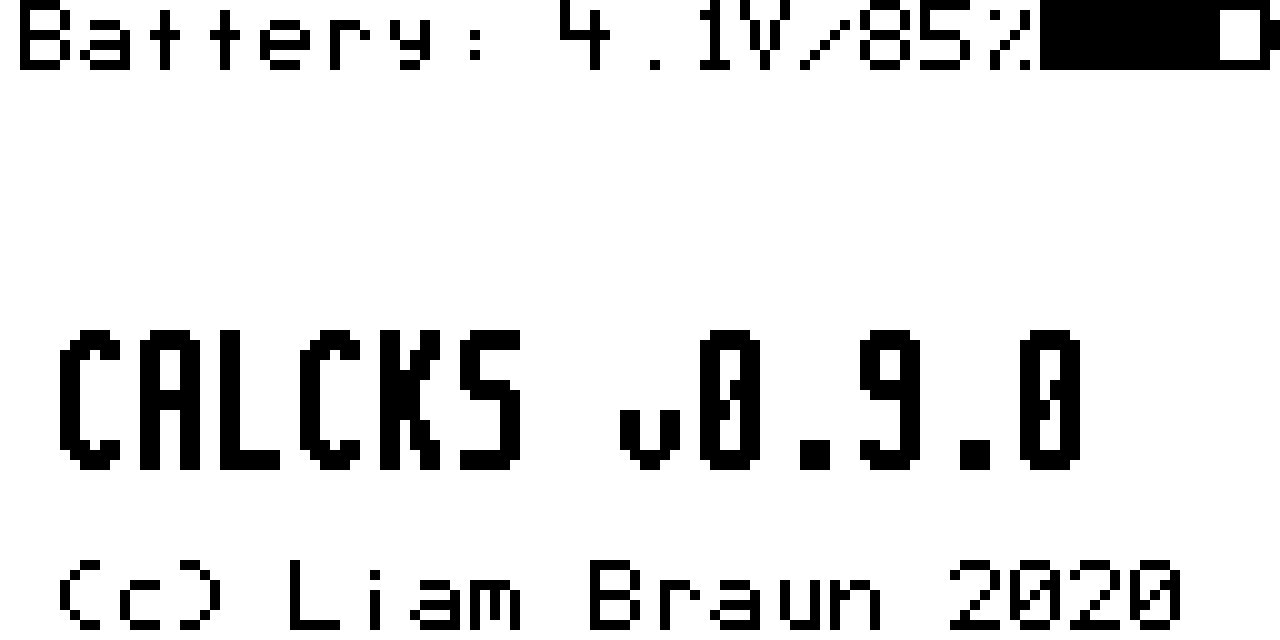
\includegraphics[width=0.4\linewidth]{assets/calc_info_l.png}}
\caption{Der Informationsbildschirm des Taschenrechners.}
\end{figure}

\noindent
Um Graphen zu zeichnen, gibt man im Hauptbildschirm einen Term ein, der $x$ enthält und drückt die f2-Taste.

\begin{figure}[H]
\fbox{
	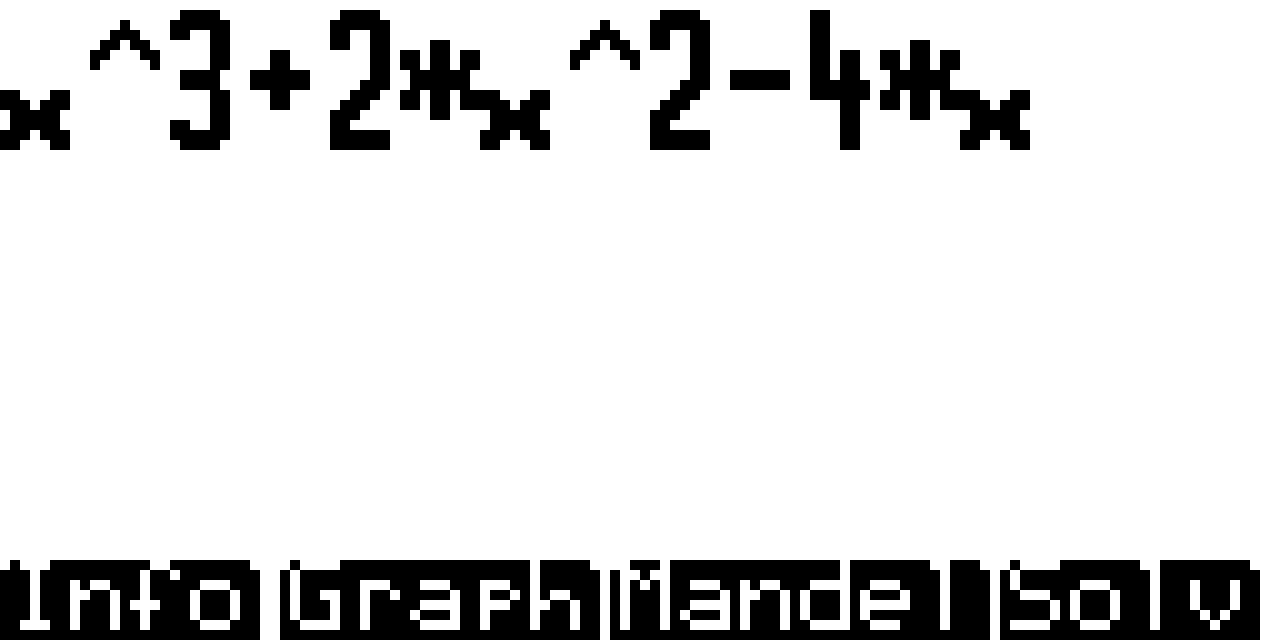
\includegraphics[width=0.4\linewidth]{assets/calc_graph_input_l.png}
}
	\hspace{2cm}
\fbox{
	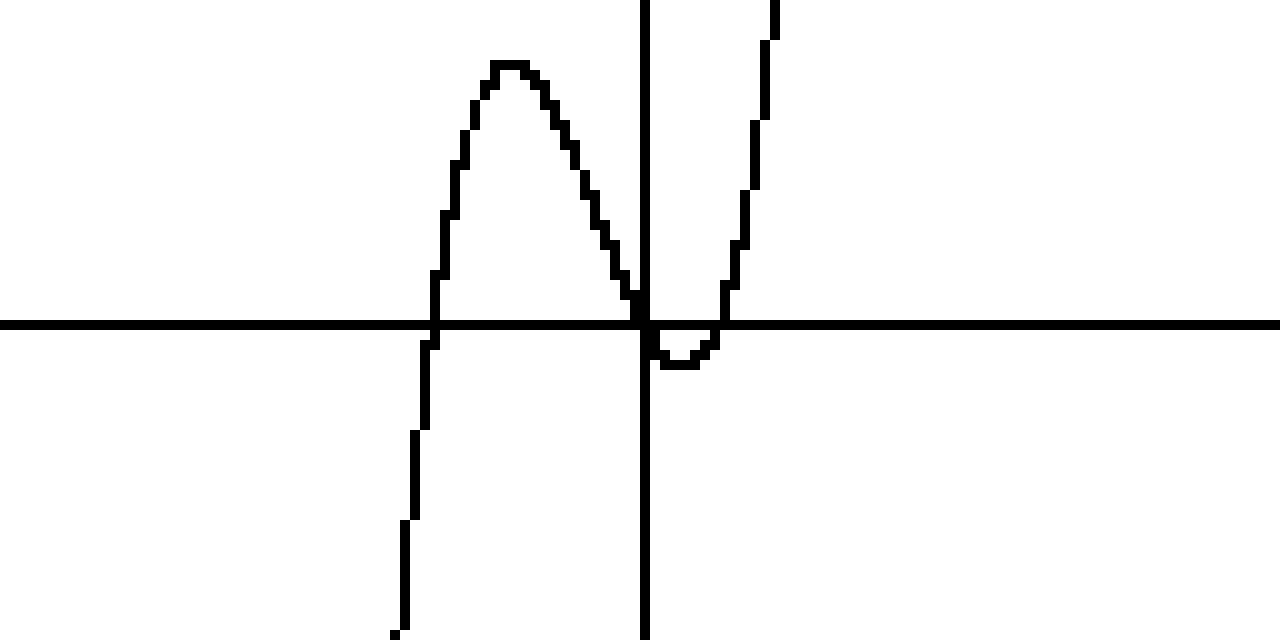
\includegraphics[width=0.4\linewidth]{assets/calc_graph_output_l.png}
}
\caption{Graphendarstellung der Gleichung $f(x)=x^3+2x^2-4x$.}
\end{figure}

\noindent
Die f3-Taste zeichnet auf dem Bildschirm das Mandelbrot-Fraktal. Diese Funktion habe ich ursprünglich geschrieben, um das Zeichnen von einzelnen Pixeln zu testen und auch die Geschwindigkeit des Rechners. Auf der Hardware, auf dem ATmega1284 mit einer Taktfrequenz von 8MHz dauert das Zeichnen des Fraktals etwa 17 Sekunden. Ich habe auch versucht, zuerst alle Pixel zu berechnen und alles gleichzeitig anzuzeigen, aber dies beschleunigte die Funktion nur um eine Sekunde, weshalb ich schlussendlich wieder auf die alte Version zurückgriff und die Pixel laufend anzeigte.

\begin{figure}[H]
\centering
\fbox{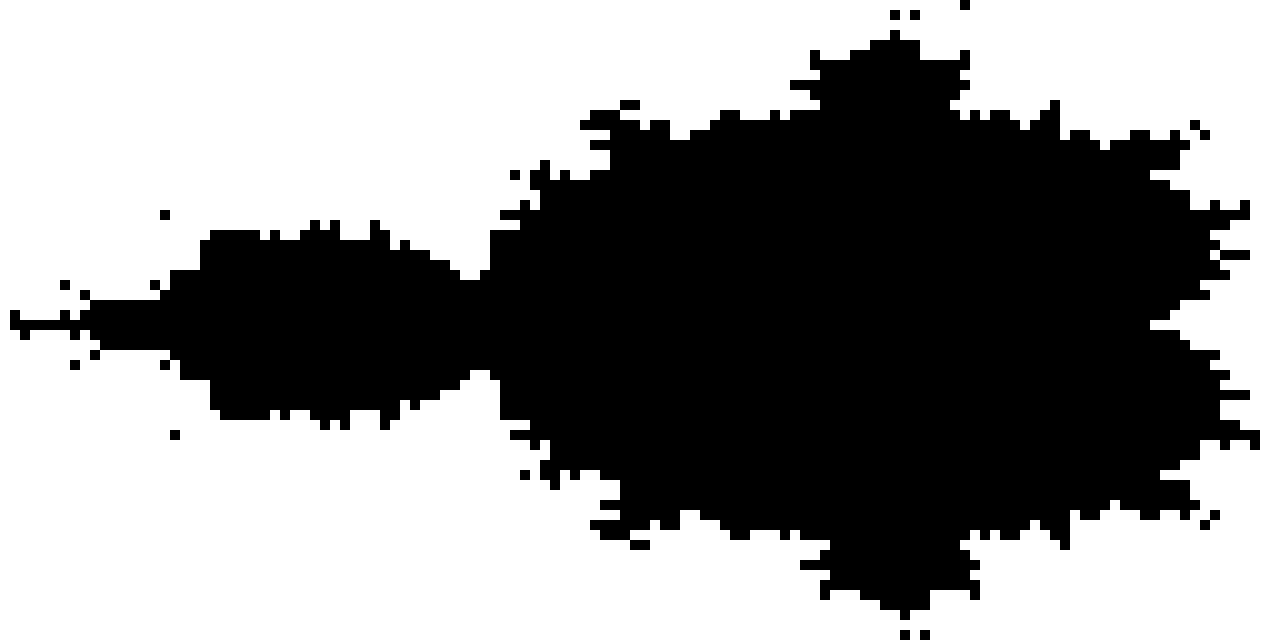
\includegraphics[width=0.4\linewidth]{assets/calc_mandelbrot_l.png}}
\caption{Das Mandelbrot-Fraktal, berechnet durch den Taschenrechner.}
\end{figure}

\newpage

\noindent
Der Taschenrechner enthält auch einen Gleichungslöser, den man mit f4 aktiviert. Momentan kann man nur lineare Gleichungen lösen, für weitere Gleichungsarten reichte die Zeit nicht. Man kann die selben Operationen wie im Hauptbildschirm verwenden, um die Werte für $m$ und $q$ einzugeben, mit der enter-Taste geht man zum nächsten Eingabefeld.

\begin{figure}[H]
\fbox{
	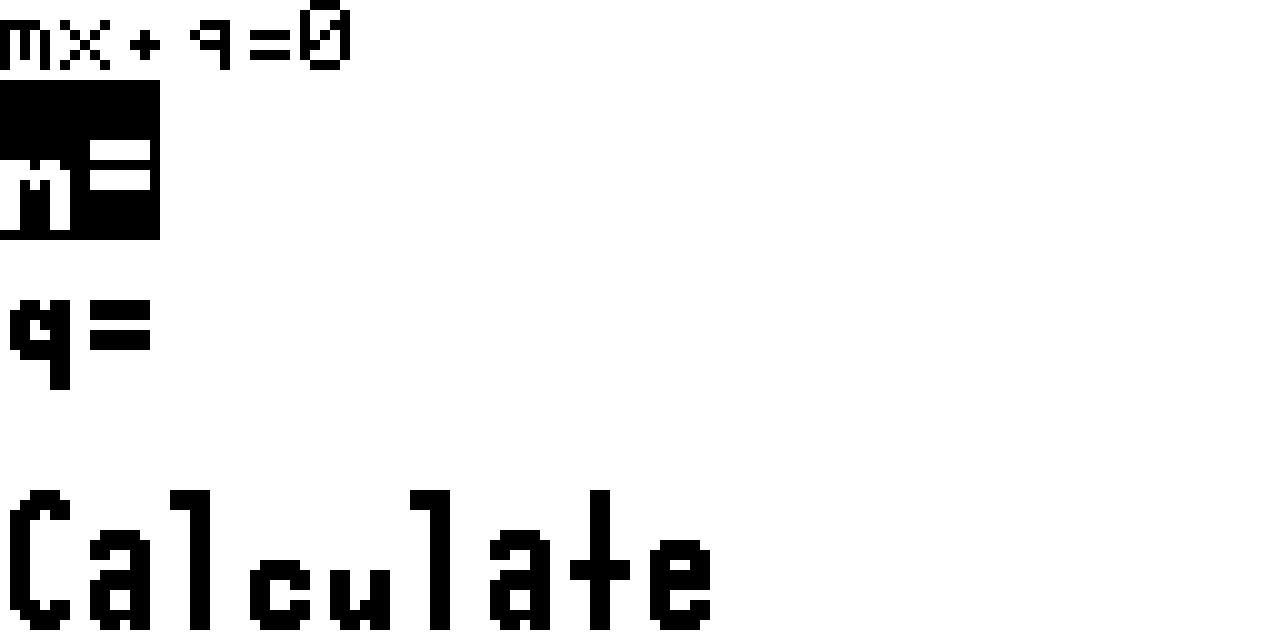
\includegraphics[width=0.28\linewidth]{assets/calc_solver_1_l.png}
}
\fbox{
	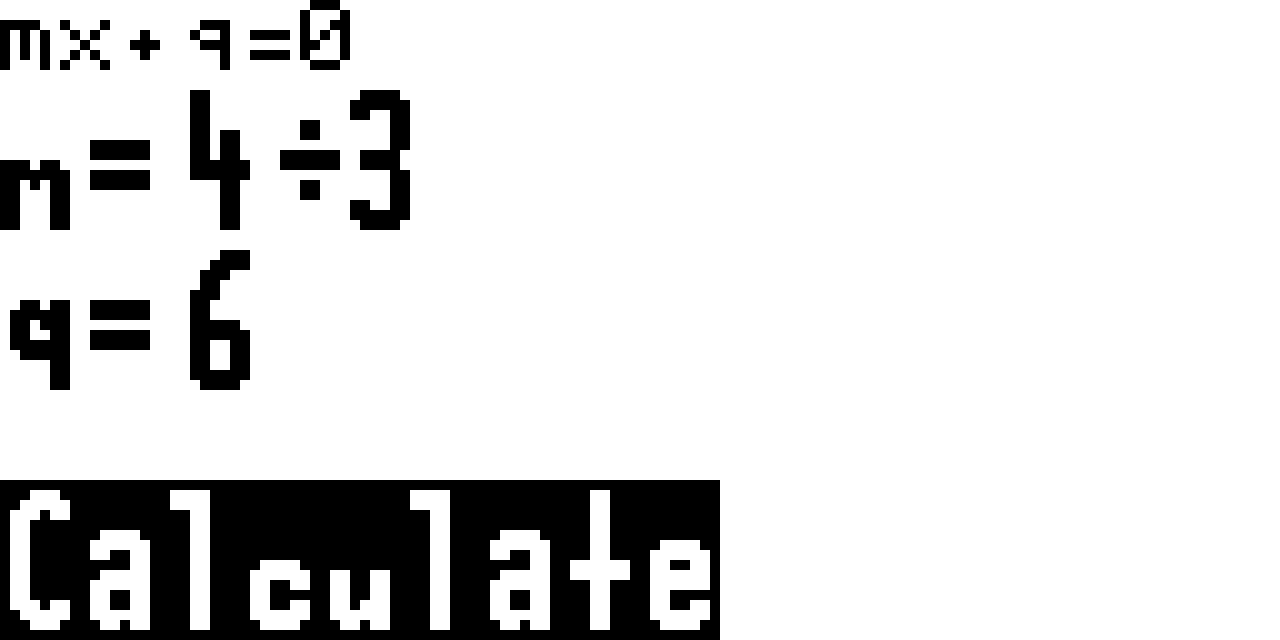
\includegraphics[width=0.28\linewidth]{assets/calc_solver_2_l.png}
}
\fbox{
	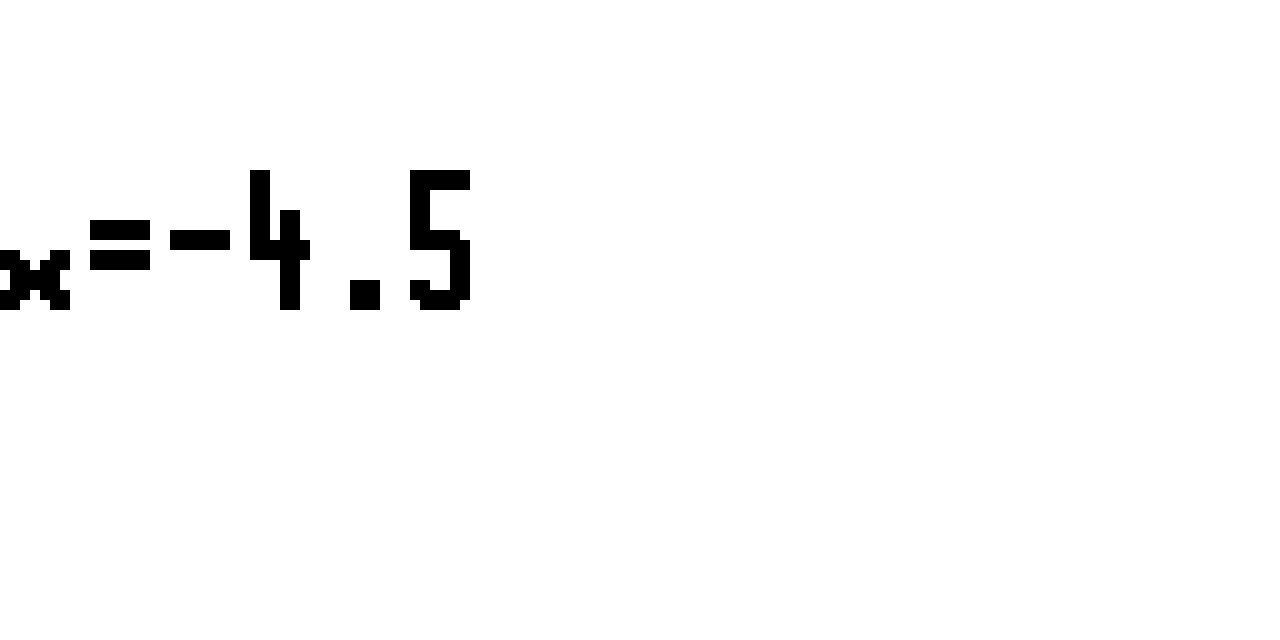
\includegraphics[width=0.28\linewidth]{assets/calc_solver_3_l.png}
}
\caption{Der Taschenrechner löst die Gleichung $\frac{4}{3}x+6=0.$}
\end{figure}

\chapter{Schlusswort}\label{excursion}
Vergleicht man das Endprodukt mit den ursprünglichen Zielen der Arbeit, findet man eine grosse Übereinstimmung.  Eine erste Anwendung fand ich bei einer Gletscherexkursion, wo meine Gruppe eine Höhenlinie von zwei Querschnitten des Rhonegletschers machen mussten. Ich konnte mir einen Drucksensor ausleihen, den ich an die Erweiterungs- und Programmierpins anschloss. Mit der Gleichung $h=44331*(1-\frac{p}{p_{0}})^{0.1903}$, wobei $h$ die gesuchte Höhe, $p$ der gemessene Luftdruck und $p_{0}$ der Luftdruck bei Meereshöhe ist, konnte laufend die Höhe über Meer bestimmt werden\footnote{Formel von \url{https://community.bosch-sensortec.com/t5/Question-and-answers/How-to-calculate-the-altitude-from-the-pressure-sensor-data/qaq-p/5702} (Abgerufen 16.10.2020)}.
\begin{center}
\begin{figure}[H]
\centering
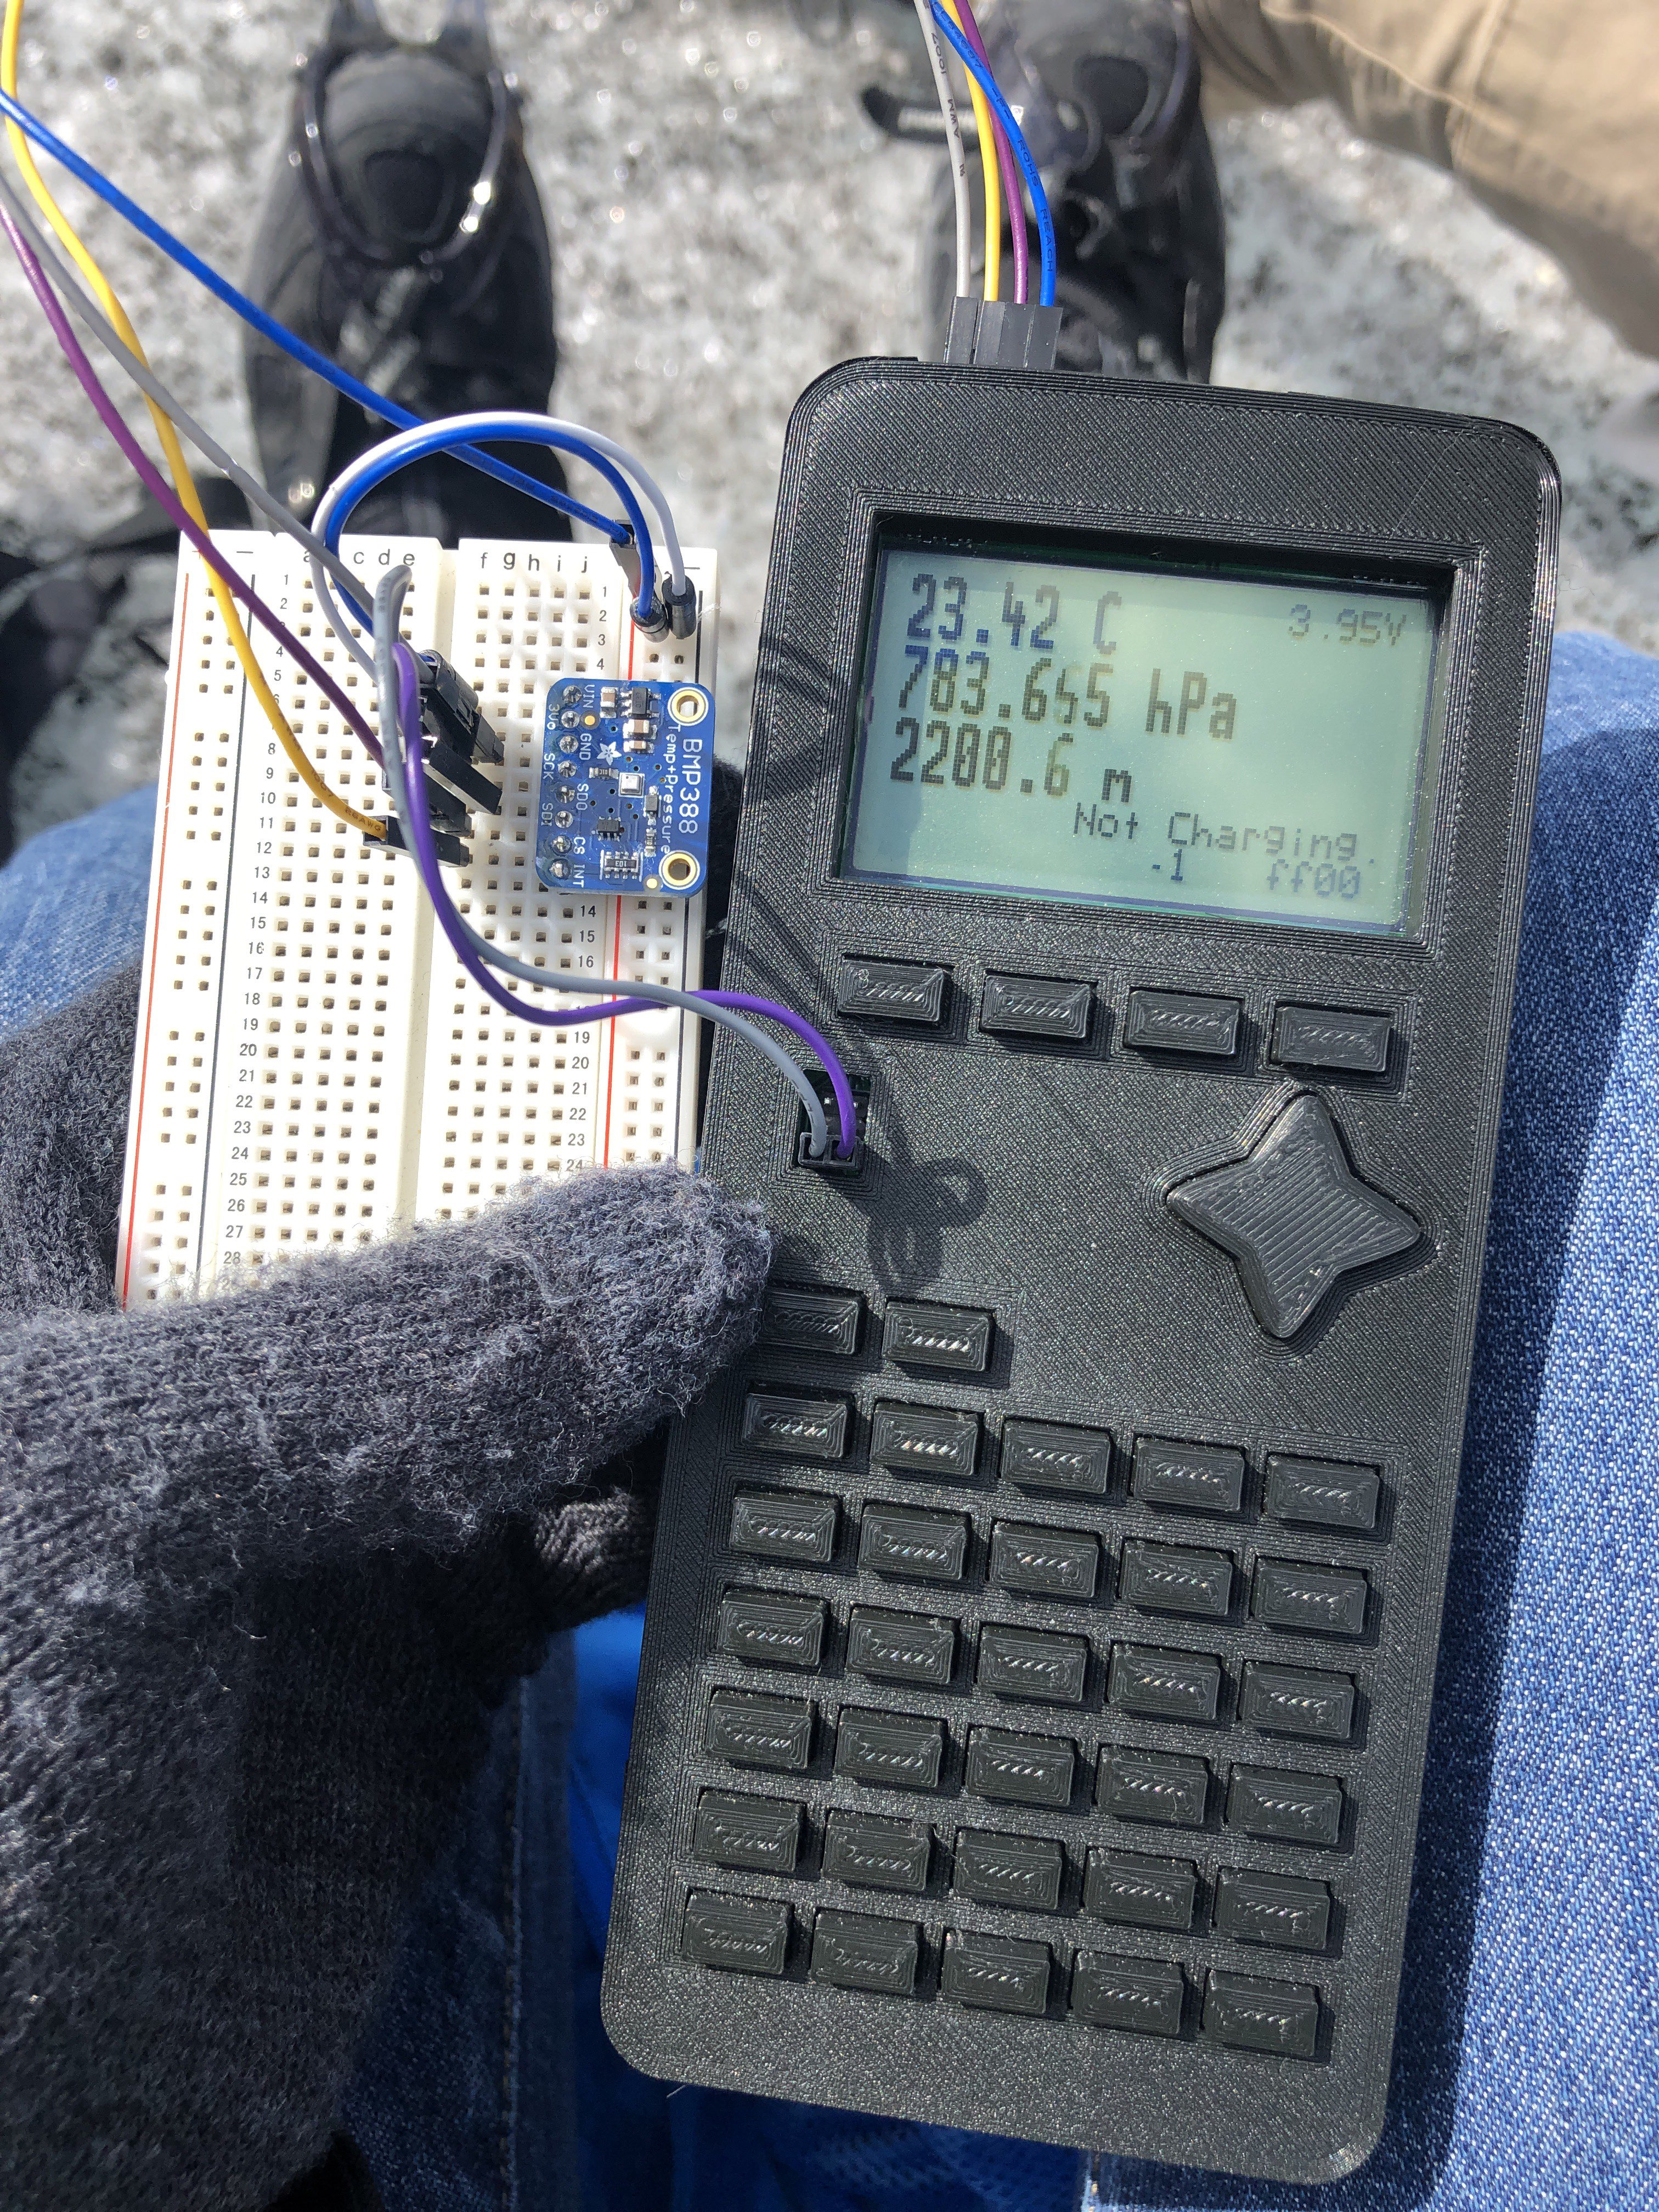
\includegraphics[width=0.45\linewidth]{assets/glacier.jpg}
\caption{Der Taschenrechner dabei auf der Gletscherexkursion.}
\end{figure}
\end{center}
Auch wenn ich gerne bei der Abgabe der Arbeit mehr Funktionalität implementiert gehabt hätte, bin ich sehr zufrieden, wie die Arbeit herausgekommen ist. Der Grund für die fehlenden Features waren nicht Hardware- oder Softwarelimitationen, sondern der Zeitdruck, der mich zwang, mich auf andere Aspekte der Arbeit zu konzentrieren. Persönlich überrascht hat mich, für welche Teile der Arbeit ich wie viel Zeit investieren musste. Ich hätte zum Beispiel nicht gedacht, dass das Anlöten der Komponenten so eine schwierige Arbeit sein werde. Hingegen war das Erfolgserlebnis, als das Anlöten ohne Brückenprobleme geklappt hat, umso grösser, weshalb ich vermutlich auch in Zukunft solche Projekt angehen werde. Ich konnte sehr viel Wertvolles über das Hardwaredesign, die Elektronik und der Informatik mitnehmen und glaube, dass ich auch nach der Abgabe noch weiterarbeiten werde, um ein nützliches Tool bei anderen Projekten zu haben. Die Maturarbeit hat mir auch insofern bei der Studienwahl geholfen, weil ich mich lange nicht zwischen den Studiengängen Informatik und Elektrotechnik \& Informationstechnologie an der ETH Zürich entscheiden konnte. Ich habe während der Arbeit bemerkt, dass mir das Programmieren und die Algorithmensuche extrem viel Spass machte, weshalb ich vorhabe, den theoretischeren der beiden Studiengänge, Informatik, zu wählen.
\chapter{Anhang}
\section{Danksagung}
Vielen Dank an meinen Betreuer Claudio Müller für die diversen Ideen für Funktionen des Taschenrechners und wertvollen Hinweise beim Schreiben des schriftlichen Teils.\\
Vielen Dank auch an Matthias Braun für das Korrekturlesen und die konstruktive Kritik an der Arbeit.
\section{Benützte Software}
Programmierumgebung: Visual Studio Code, Version 1.49.3 \\
PCB Design: KiCad, Version 5.1.5 \\
CAD: Autodesk Fusion 360 mit Studentenlizenz, Version 2.0.9009 \\
C-Compiler für ATmega: WinAVR, Version 20090313 \\
AVR Uploader: avrdude, Version 5.10 \\
Design der Schriftart und Logo: Aseprite, Version 1.2.25-x64 \\
Illustrationen für den schriftlichen Teil: Inkscape, Version 1.0 \\
Darstellung der Bill of Materials: Microsoft Excel für Microsoft 365 \\
Schriftlicher Teil: Geschrieben und kompiliert mit Texmaker, Version 5.0.4

\section{Anmerkung zu Abbildungen}
Abbildung \ref{fig:mewithcalc} ist von Matthias Braun fotografiert.\\
Abbildung \ref{fig:button_image} stammt von DigiKey Electronics und ist unter \url{https://www.digikey.ch/product-detail/de/e-switch/TL3301SPF260QG/EG1870CT-ND/271567} (Abgerufen 16.10.2020) zu finden.\\
Die gerenderten PCB-Layouts im Anhang wurden mit \url{https://www.gerblook.org/} (Aufgerufen 14.10.2020) von den selbsterstellten Projektdateien generiert.\\
Alle anderen in dieser Arbeit verwendeten Abbildungen sind von dem Autor mit den erwähnten Programmen selbst erstellt worden.

\begin{landscape}
\section{Stückliste}
Diese Liste wurde automatisch von KiCad generiert und besteht aus allen Komponenten, die im Schema aufgelistet sind. Dies beinhaltet den Akku nicht, weil im Schema für diesen nur die dazugehörigen Lötpads eingetragen sind.
\begin{figure}[h]
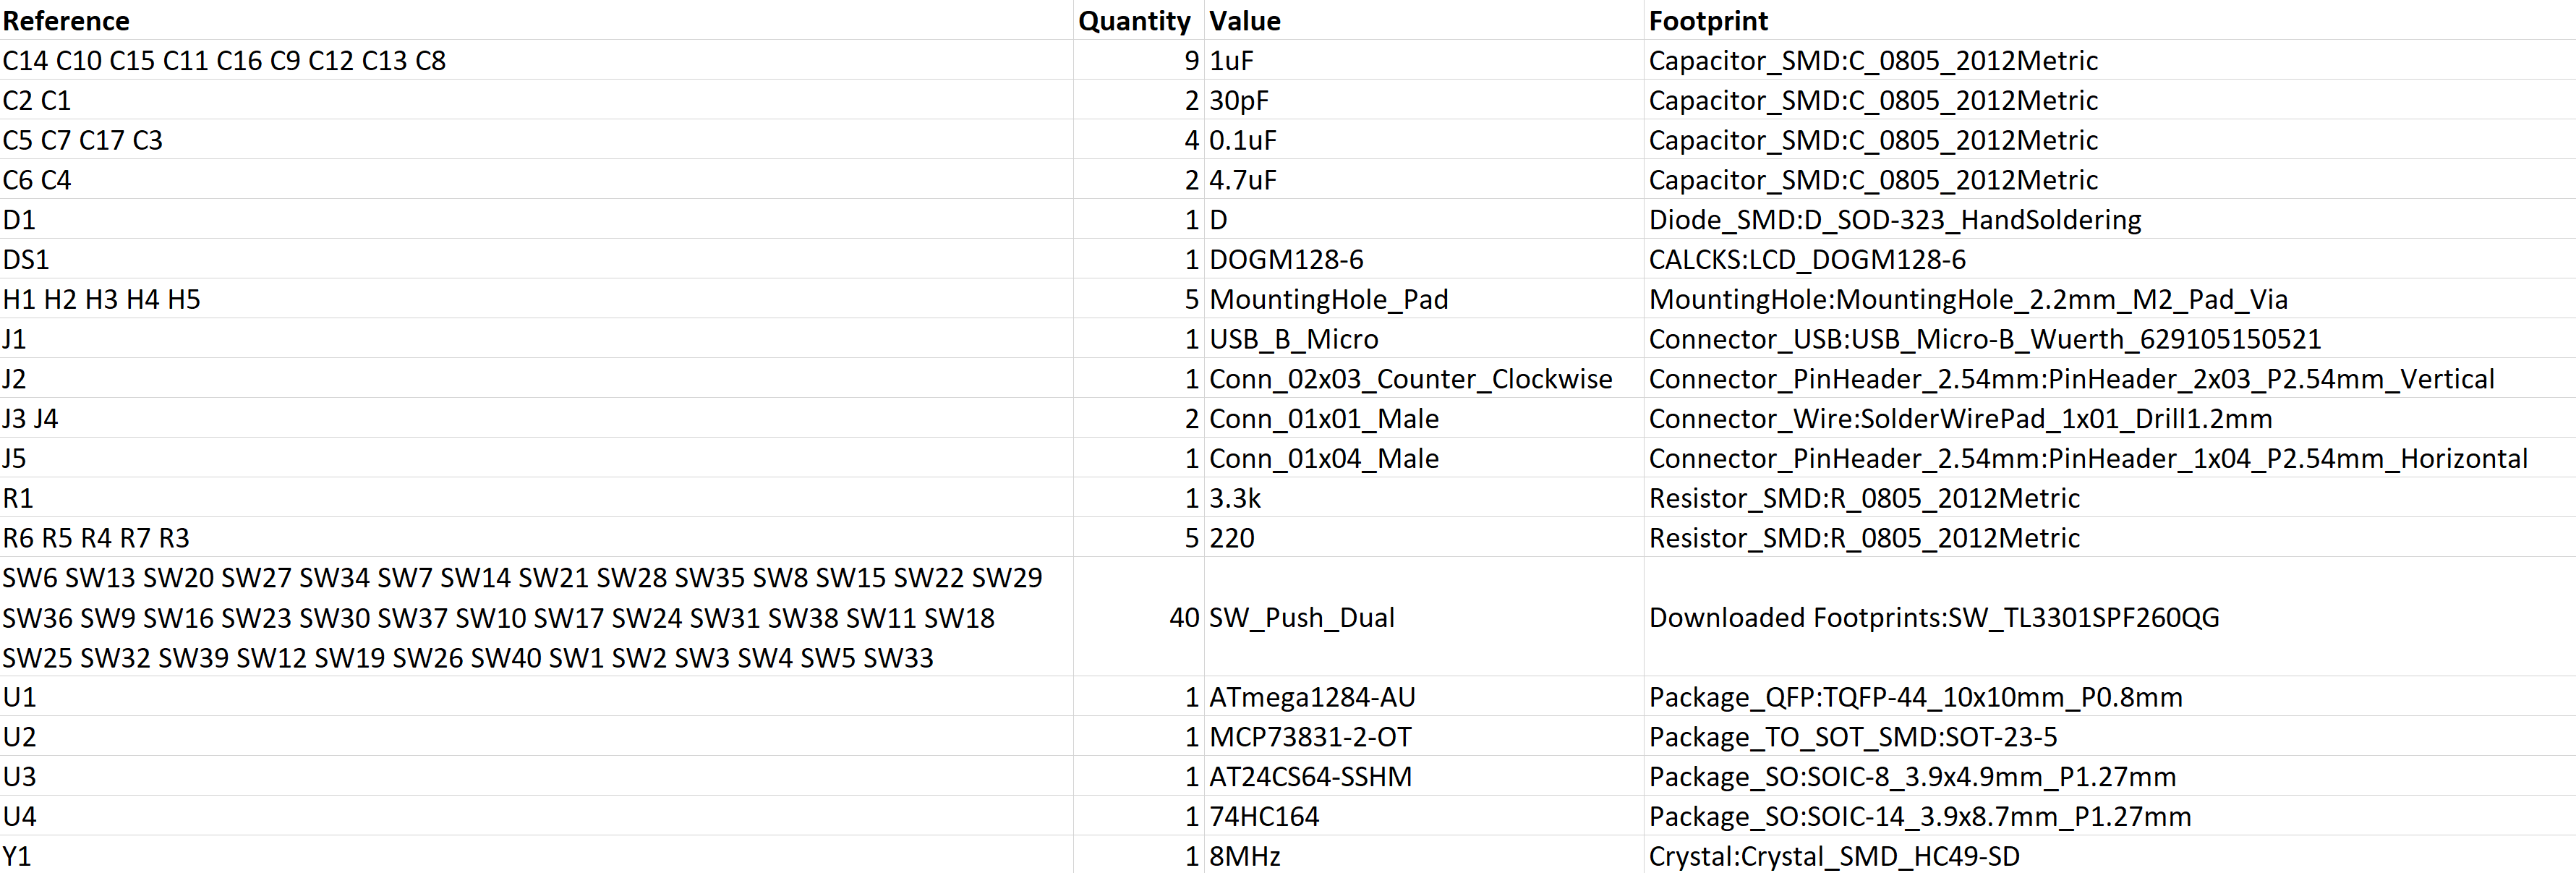
\includegraphics[width=\linewidth]{assets/bom.png}
\end{figure}
\newpage
\section{Schema}
\begin{figure}[H]
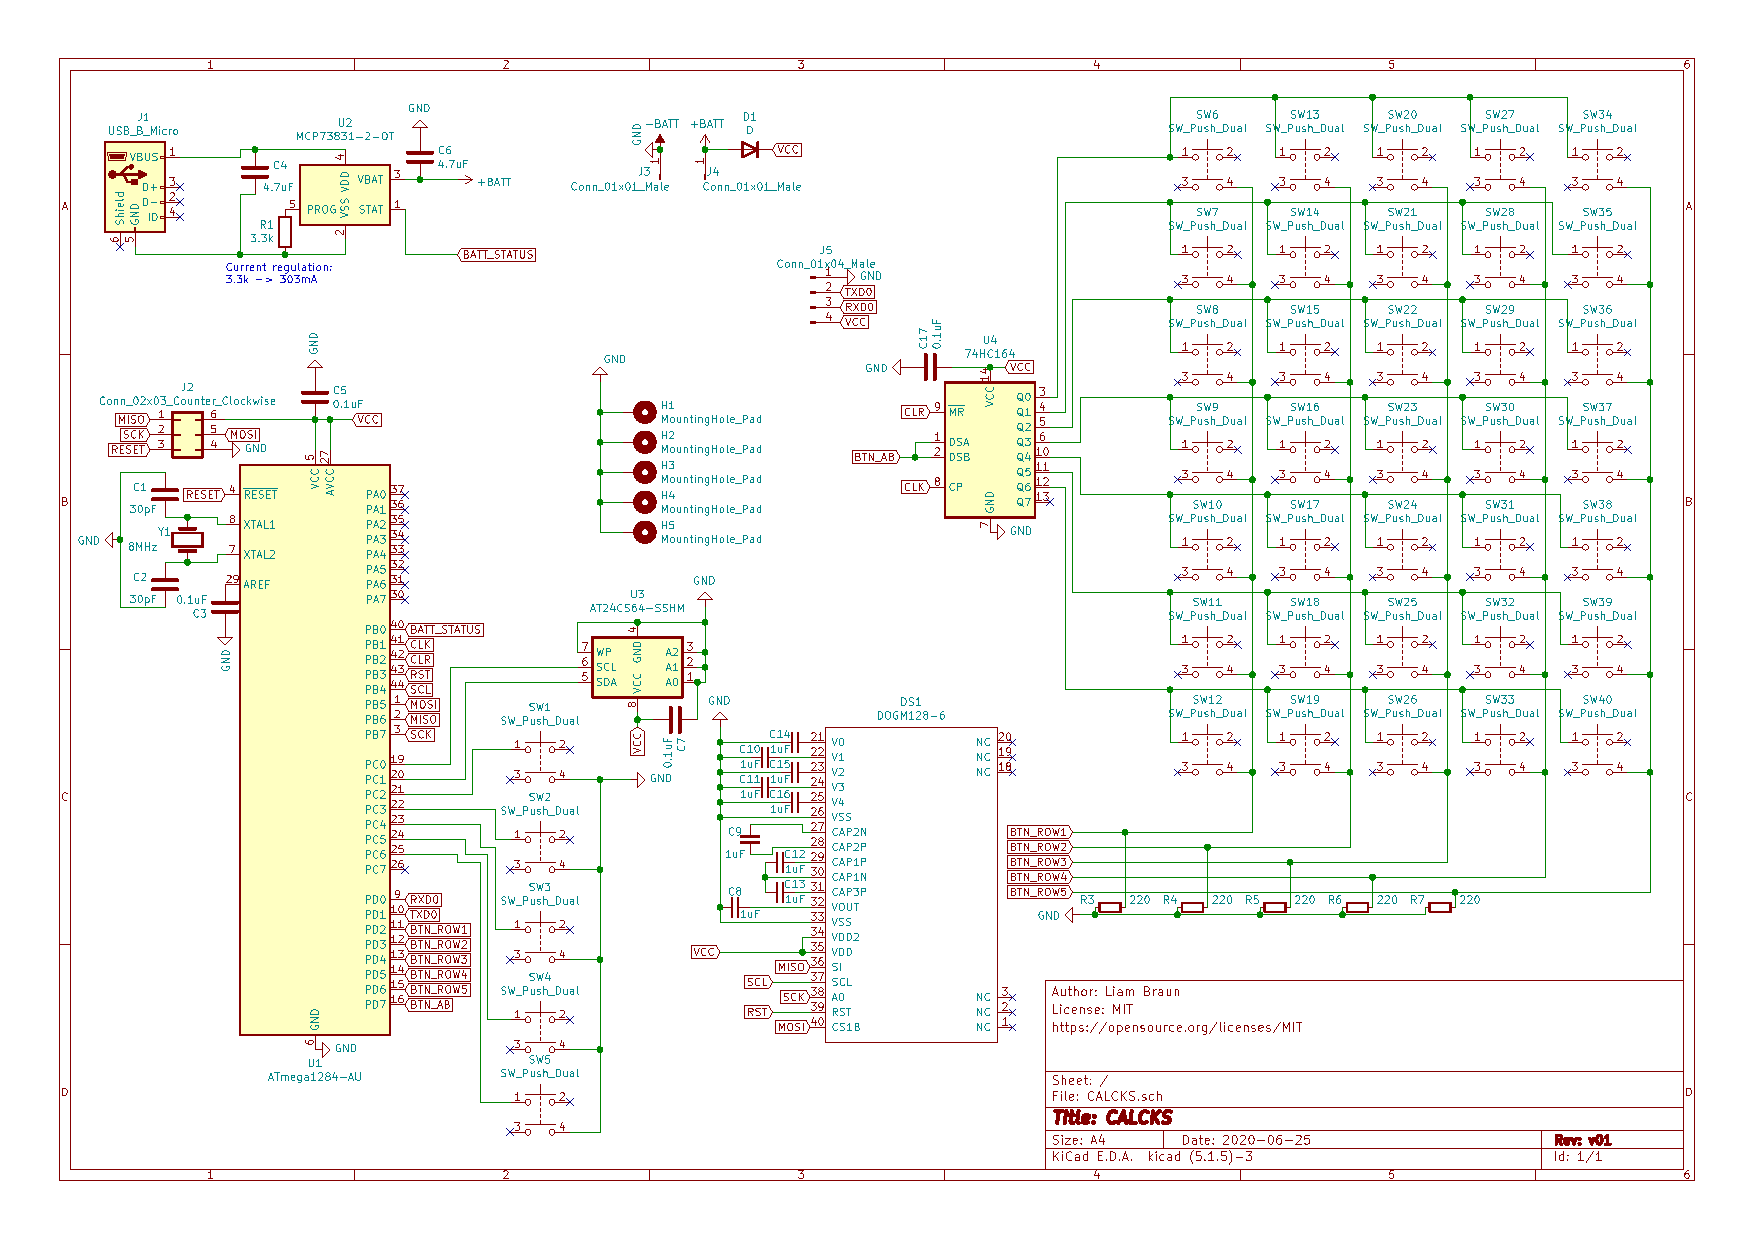
\includegraphics[height=\textheight]{assets/schematic.pdf}
\end{figure}
\end{landscape}
\section{PCB Render}
\nopagebreak
\begin{figure}[H]
	\centering
	\subfloat[\centering Vorderseite]{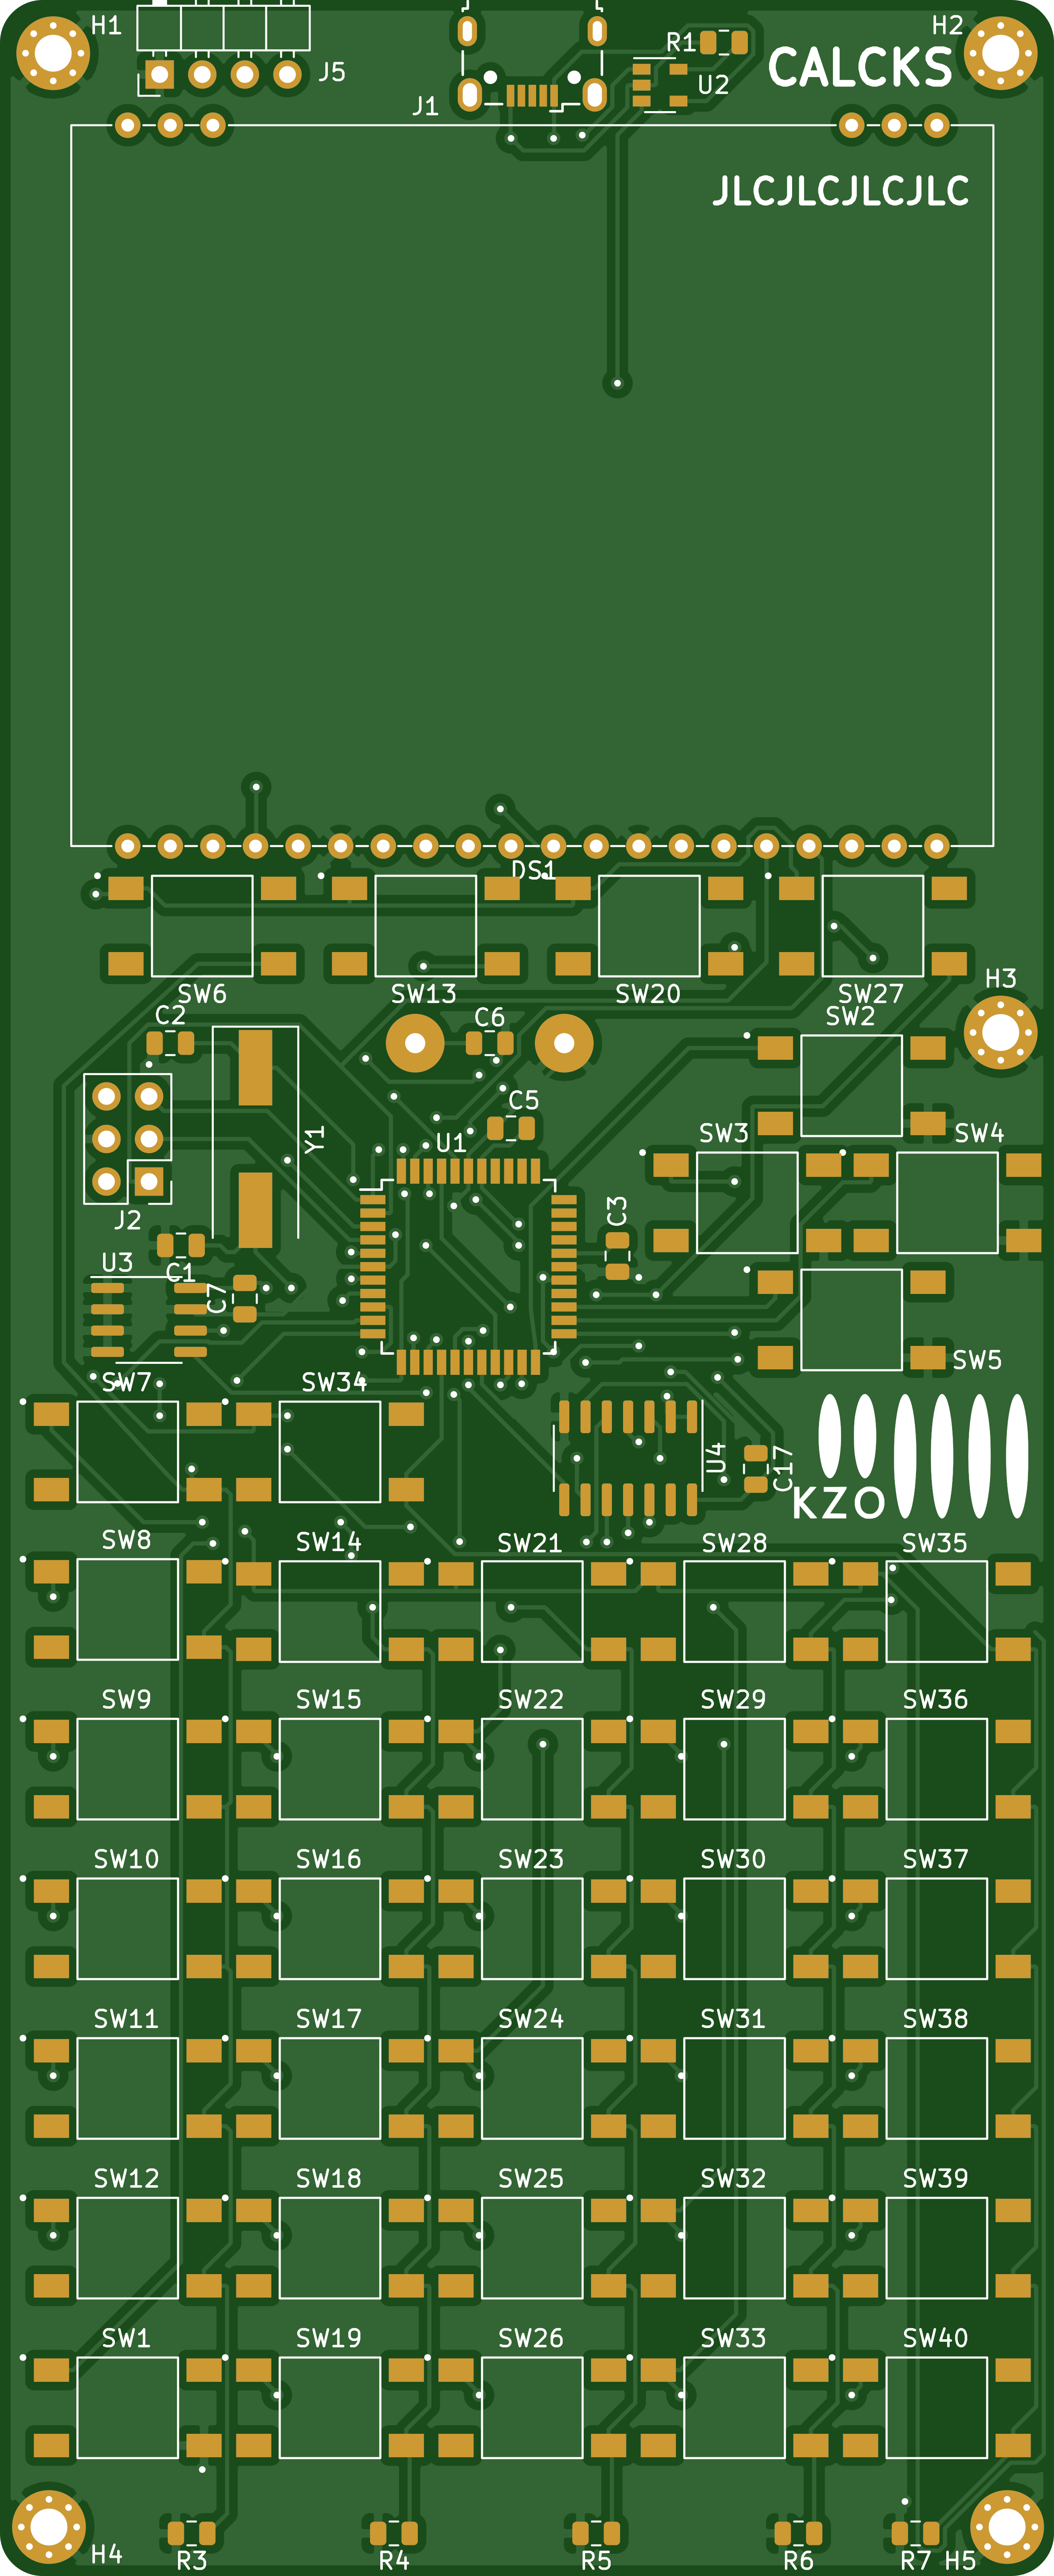
\includegraphics[height=0.7\textheight]{assets/top.png}}%
    \qquad
    \subfloat[\centering Rückseite]{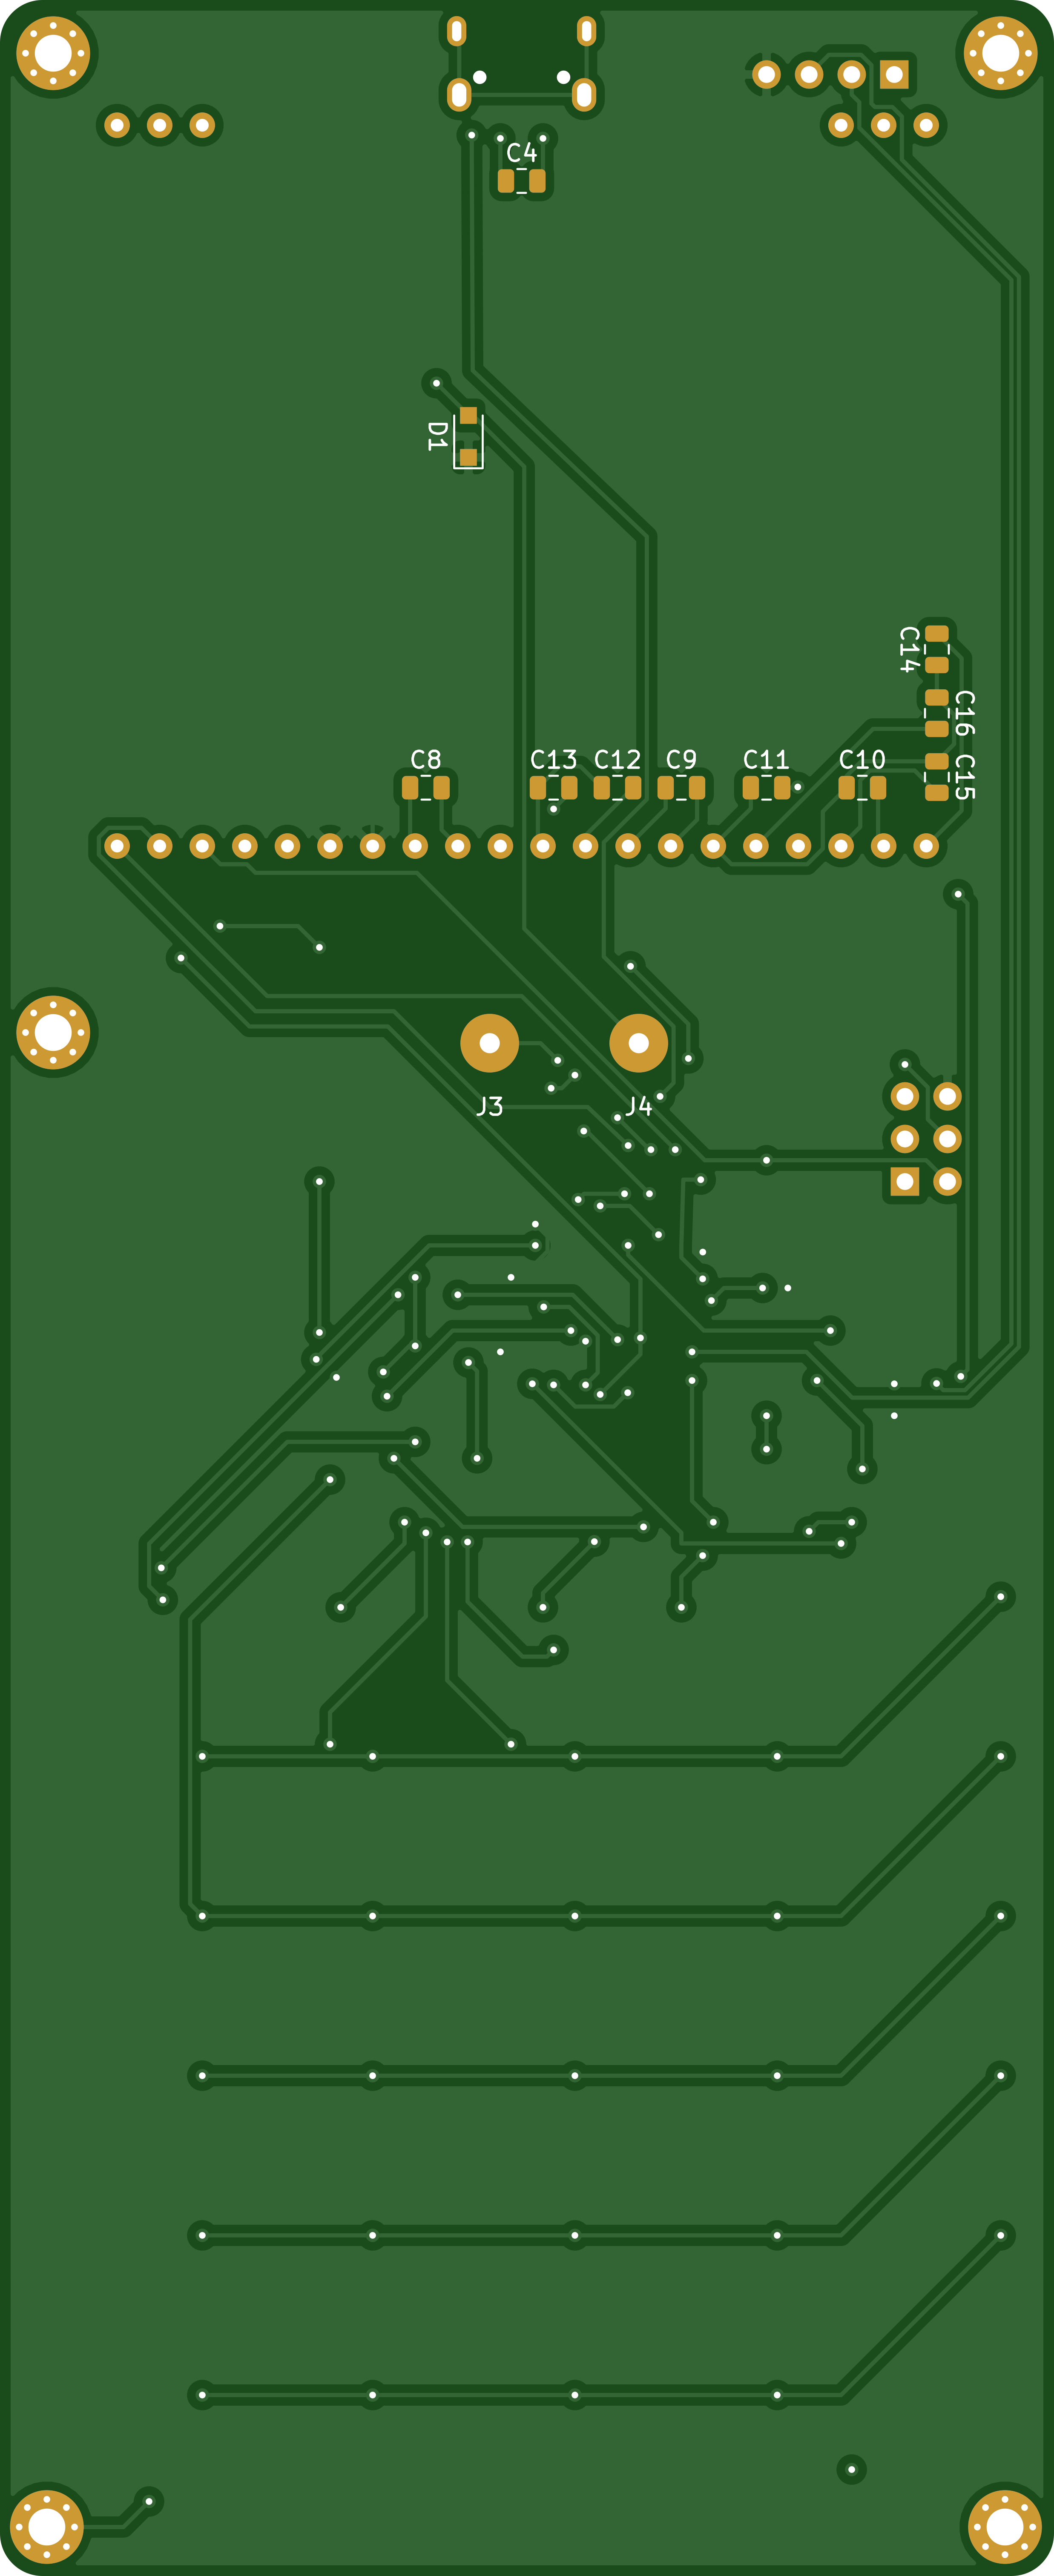
\includegraphics[height=0.7\textheight]{assets/bottom.png}}%
    \label{fig:pcbrenders}%
\end{figure}

\bibliography{calcks}
\bibliographystyle{plain}
\nocite{*}

\end{document}